% generated from JIRA project LVV
% using template at /usr/share/miniconda/envs/docsteady-env/lib/python3.7/site-packages/docsteady/templates/tpr.latex.jinja2.
% using docsteady version 2.2.4
% Please do not edit -- update information in Jira instead
\documentclass[dm,lsstdraft,STR,toc]{lsstdoc}
\usepackage{geometry}
\usepackage{longtable,booktabs}
\usepackage{enumitem}
\usepackage{arydshln}
\usepackage{attachfile}
\usepackage{array}
\usepackage{dashrule}

\newcolumntype{L}[1]{>{\raggedright\let\newline\\\arraybackslash\hspace{0pt}}p{#1}}

\input meta.tex

\newcommand{\attachmentsUrl}{https://github.com/\gitorg/\lsstDocType-\lsstDocNum/blob/\gitref/attachments}
\providecommand{\tightlist}{
  \setlength{\itemsep}{0pt}\setlength{\parskip}{0pt}}

\setcounter{tocdepth}{4}

\begin{document}

\def\milestoneName{Gen 3 Butler Acceptance Testing}
\def\milestoneId{LDM-GEN3}
\def\product{Software Products}

\setDocCompact{true}

\title{LDM-GEN3: Gen 3 Butler Acceptance Testing Test Plan and Report}
\setDocRef{\lsstDocType-\lsstDocNum}
\date{ 2022-04-21 }
\author{ Robert Gruendl }

% Most recent last
\setDocChangeRecord{
\addtohist{}{2020-10-30}{First draft}{Robert Gruendl}
\addtohist{}{2021-01-28}{Include new test cycle for LDM-556 requirements}{Leanne Guy}
\addtohist{}{2022-06-07}{Test campaign LVV-P77 completed and results approved. DM-27337}
}

\setDocCurator{Jeff Carlin}
\setDocUpstreamLocation{\url{https://github.com/lsst-dm/\lsstDocType-\lsstDocNum}}
\setDocUpstreamVersion{\vcsrevision}



\setDocAbstract{
This is the test plan and report for
\textbf{ Gen 3 Butler Acceptance Testing} (LDM-GEN3),
an LSST milestone pertaining to the Data Management Subsystem.\\
This document is based on content automatically extracted from the Jira test database on \docDate.
The most recent change to the document repository was on \vcsDate.
}


\maketitle

\section{Introduction}
\label{sect:intro}


\subsection{Objectives}
\label{sect:objectives}

 The goal of this test is to demonstrate that the Gen3 Butler software
project has sufficiently matured that subsequent DM development should
begin focusing on adoption of Gen3 Butler software are repositories
throughout the DM software project (i.e. that deprecation of Gen2 Butler
usage within the project can begin).



\subsection{System Overview}
\label{sect:systemoverview}

 The Gen3 refactoring of the Butler is central to evolution of the
overall DM software design and has repercussions throughout the rest of
the DM project. ~ This test plan is designed to verify that minimal
requirements have been met and the DM project can now begin the process
of integrating the Gen3 Butler within the pipelines and analysis tools.
~ Those minimal requirements are that:

\begin{enumerate}
\tightlist
\item
  possible to ingest raw dataset types central to the Rubin operations
  and the ongoing development of the data management systems..
\item
  cp\_pipe equivalent under Gen3 is available
\item
  developers can run a pipeline with a single-node using pipetask
\item
  processing supporting development is possible in a reasonable time
  (e.g. a 3-tract RC2 test run can be accomplished within a reasonable
  time)~
\item
  Calibration Product Pipelines (CPP) can be run to support above
  investigations
\item
  Batch Processing System (BPS) is available to support testing at
  larger scales
\end{enumerate}

In addition, at the time these tests occur the Gen3 Butler schema be
considered stable enough that changes no longer occur on a weekly basis
(i.e forced re-ingestion/migration of existing repositories are no
longer a weekly occurrence). Changes requiring wholesale
reingestion/migration may still be required but will occur in a
regimented manner and the choice to allow schema changes without an
accompanying means to migrate old repositories would become a
change-control board (CCB) level
issue.\\[2\baselineskip]\textbf{Applicable Documents:}\\
\citeds{LDM-592}: Data Access Use Cases\\
\citeds{LDM-556}: Data Management Middleware Requirements\\
\citeds{LDM-639}: Data Management Acceptance Test Specification\\[2\baselineskip]


\subsection{Document Overview}
\label{sect:docoverview}

This document was generated from Jira, obtaining the relevant information from the
\href{https://jira.lsstcorp.org/secure/Tests.jspa\#/testPlan/LVV-P77}{LVV-P77}
~Jira Test Plan and related Test Cycles (
\href{https://jira.lsstcorp.org/secure/Tests.jspa\#/testCycle/LVV-C160}{LVV-C160}
\href{https://jira.lsstcorp.org/secure/Tests.jspa\#/testCycle/LVV-C162}{LVV-C162}
\href{https://jira.lsstcorp.org/secure/Tests.jspa\#/testCycle/LVV-C190}{LVV-C190}
).

Section \ref{sect:intro} provides an overview of the test campaign, the system under test (\product{}),
the applicable documentation, and explains how this document is organized.
Section \ref{sect:testplan} provides additional information about the test plan, like for example the configuration
used for this test or related documentation.
Section \ref{sect:personnel} describes the necessary roles and lists the individuals assigned to them.

Section \ref{sect:overview} provides a summary of the test results, including an overview in Table \ref{table:summary},
an overall assessment statement and suggestions for possible improvements.
Section \ref{sect:detailedtestresults} provides detailed results for each step in each test case.

The current status of test plan \href{https://jira.lsstcorp.org/secure/Tests.jspa\#/testPlan/LVV-P77}{LVV-P77} in Jira is \textbf{ Draft }.

\subsection{References}
\label{sect:references}
\renewcommand{\refname}{}
\bibliography{lsst,refs,books,refs_ads,local}


\newpage
\section{Test Plan Details}
\label{sect:testplan}


\subsection{Data Collection}

  Observing is not required for this test campaign.

\subsection{Verification Environment}
\label{sect:hwconf}
  These tests assume a stable weekly stack which supports Gen3 running of
the above, that services that automatically ingest new data can support
on-going ingestion to Gen3 repositories (i.e. DBB shared spaces and OODS
support serving data through Gen3), and that batch processing services
can support pipeline execution of Gen3 products.




\subsection{Related Documentation}


\begin{longtable}{rp{10cm}l}
\multicolumn{3}{c}{Jira Attachments} \\ \hline
 To LVV-C160 results &
  DM-Gen2MiddlewareRemovalPlanning-080222-2302-1360.pdf & \attachfile{attachments/DM-Gen2MiddlewareRemovalPlanning-080222-2302-1360.pdf}\\ \hline
  To LVV-C160 results &
  DRP.yaml & \attachfile{attachments/DRP.yaml}\\ \hline
To LVV-C160 results &
  DRP-RC2.yaml & \attachfile{attachments/DRP-RC2.yaml}\\ \hline
To LVV-C160 results &
  DRP-ci\_hsc+fakes.yaml & \attachfile{attachments/DRP-ci_hsc+fakes.yaml}\\ \hline
To LVV-C160 results &
  pipeline\_detail.png & \attachfile{attachments/pipeline_detail.png}\\ \hline
To LVV-C160 results &
  pipeline.png & \attachfile{attachments/pipeline.png}\\ \hline
To LVV-C160 results &
  ci\_hsc\_log\_w\_2022\_05.log & \attachfile{attachments/ci_hsc_log_w_2022_05.log}\\ \hline
                                                                     \end{longtable}

All documents provided as attachments in Jira are downloaded to Github and linked here for convenience.
However, since they are not properly versioned, they should be considered informal and therefore
not be part of the verification baseline.


\subsection{PMCS Activity}

Primavera milestones related to the test campaign:
\begin{itemize}
\item LDM-GEN3
\end{itemize}


\newpage
\section{Personnel}
\label{sect:personnel}

The personnel involved in the test campaign is shown in the following table.

{\small
\begin{longtable}{p{3cm}p{3cm}p{3cm}p{6cm}}
\hline
\multicolumn{2}{r}{T. Plan \href{https://jira.lsstcorp.org/secure/Tests.jspa\#/testPlan/LVV-P77}{LVV-P77} owner:} &
\multicolumn{2}{l}{\textbf{ Robert Gruendl } }\\\hline
\multicolumn{2}{r}{T. Cycle \href{https://jira.lsstcorp.org/secure/Tests.jspa\#/testCycle/LVV-C160}{LVV-C160} owner:} &
\multicolumn{2}{l}{\textbf{
Robert Gruendl }
} \\\hline
\textbf{Test Cases} & \textbf{Assigned to} & \textbf{Executed by} & \textbf{Additional Test Personnel} \\ \hline
\href{https://jira.lsstcorp.org/secure/Tests.jspa#/testCase/LVV-T2264}{LVV-T2264}
& {\small Leanne Guy } & {\small Jeffrey Carlin } &
\begin{minipage}[]{6cm}
\smallskip
{\small  }
\medskip
\end{minipage}
\\ \hline
\href{https://jira.lsstcorp.org/secure/Tests.jspa#/testCase/LVV-T1984}{LVV-T1984}
& {\small Leanne Guy } & {\small Jeffrey Carlin } &
\begin{minipage}[]{6cm}
\smallskip
{\small  }
\medskip
\end{minipage}
\\ \hline
\href{https://jira.lsstcorp.org/secure/Tests.jspa#/testCase/LVV-T1982}{LVV-T1982}
& {\small Leanne Guy } & {\small Jeffrey Carlin } &
\begin{minipage}[]{6cm}
\smallskip
{\small  }
\medskip
\end{minipage}
\\ \hline
\href{https://jira.lsstcorp.org/secure/Tests.jspa#/testCase/LVV-T1987}{LVV-T1987}
& {\small Leanne Guy } & {\small Jeffrey Carlin } &
\begin{minipage}[]{6cm}
\smallskip
{\small  }
\medskip
\end{minipage}
\\ \hline
\href{https://jira.lsstcorp.org/secure/Tests.jspa#/testCase/LVV-T1983}{LVV-T1983}
& {\small Leanne Guy } & {\small Jeffrey Carlin } &
\begin{minipage}[]{6cm}
\smallskip
{\small  }
\medskip
\end{minipage}
\\ \hline
\multicolumn{2}{r}{T. Cycle \href{https://jira.lsstcorp.org/secure/Tests.jspa\#/testCycle/LVV-C162}{LVV-C162} owner:} &
\multicolumn{2}{l}{\textbf{
Undefined }
} \\\hline
\textbf{Test Cases} & \textbf{Assigned to} & \textbf{Executed by} & \textbf{Additional Test Personnel} \\ \hline
\href{https://jira.lsstcorp.org/secure/Tests.jspa#/testCase/LVV-T1985}{LVV-T1985}
& {\small Leanne Guy } & {\small  } &
\begin{minipage}[]{6cm}
\smallskip
{\small  }
\medskip
\end{minipage}
\\ \hline
\multicolumn{2}{r}{T. Cycle \href{https://jira.lsstcorp.org/secure/Tests.jspa\#/testCycle/LVV-C190}{LVV-C190} owner:} &
\multicolumn{2}{l}{\textbf{
Jeffrey Carlin }
} \\\hline
\textbf{Test Cases} & \textbf{Assigned to} & \textbf{Executed by} & \textbf{Additional Test Personnel} \\ \hline
\href{https://jira.lsstcorp.org/secure/Tests.jspa#/testCase/LVV-T2503}{LVV-T2503}
& {\small Leanne Guy } & {\small  } &
\begin{minipage}[]{6cm}
\smallskip
{\small  }
\medskip
\end{minipage}
\\ \hline
\href{https://jira.lsstcorp.org/secure/Tests.jspa#/testCase/LVV-T2502}{LVV-T2502}
& {\small Leanne Guy } & {\small  } &
\begin{minipage}[]{6cm}
\smallskip
{\small  }
\medskip
\end{minipage}
\\ \hline
\href{https://jira.lsstcorp.org/secure/Tests.jspa#/testCase/LVV-T2501}{LVV-T2501}
& {\small Leanne Guy } & {\small  } &
\begin{minipage}[]{6cm}
\smallskip
{\small  }
\medskip
\end{minipage}
\\ \hline
\href{https://jira.lsstcorp.org/secure/Tests.jspa#/testCase/LVV-T2499}{LVV-T2499}
& {\small Leanne Guy } & {\small  } &
\begin{minipage}[]{6cm}
\smallskip
{\small  }
\medskip
\end{minipage}
\\ \hline
\href{https://jira.lsstcorp.org/secure/Tests.jspa#/testCase/LVV-T2498}{LVV-T2498}
& {\small Leanne Guy } & {\small Jeffrey Carlin } &
\begin{minipage}[]{6cm}
\smallskip
{\small  }
\medskip
\end{minipage}
\\ \hline
\href{https://jira.lsstcorp.org/secure/Tests.jspa#/testCase/LVV-T2497}{LVV-T2497}
& {\small Leanne Guy } & {\small Jeffrey Carlin } &
\begin{minipage}[]{6cm}
\smallskip
{\small  }
\medskip
\end{minipage}
\\ \hline
\href{https://jira.lsstcorp.org/secure/Tests.jspa#/testCase/LVV-T2496}{LVV-T2496}
& {\small Leanne Guy } & {\small  } &
\begin{minipage}[]{6cm}
\smallskip
{\small  }
\medskip
\end{minipage}
\\ \hline
\href{https://jira.lsstcorp.org/secure/Tests.jspa#/testCase/LVV-T2495}{LVV-T2495}
& {\small Leanne Guy } & {\small  } &
\begin{minipage}[]{6cm}
\smallskip
{\small  }
\medskip
\end{minipage}
\\ \hline
\href{https://jira.lsstcorp.org/secure/Tests.jspa#/testCase/LVV-T2494}{LVV-T2494}
& {\small Leanne Guy } & {\small  } &
\begin{minipage}[]{6cm}
\smallskip
{\small  }
\medskip
\end{minipage}
\\ \hline
\href{https://jira.lsstcorp.org/secure/Tests.jspa#/testCase/LVV-T2493}{LVV-T2493}
& {\small Leanne Guy } & {\small  } &
\begin{minipage}[]{6cm}
\smallskip
{\small  }
\medskip
\end{minipage}
\\ \hline
\href{https://jira.lsstcorp.org/secure/Tests.jspa#/testCase/LVV-T2492}{LVV-T2492}
& {\small Leanne Guy } & {\small  } &
\begin{minipage}[]{6cm}
\smallskip
{\small  }
\medskip
\end{minipage}
\\ \hline
\href{https://jira.lsstcorp.org/secure/Tests.jspa#/testCase/LVV-T2491}{LVV-T2491}
& {\small Leanne Guy } & {\small  } &
\begin{minipage}[]{6cm}
\smallskip
{\small  }
\medskip
\end{minipage}
\\ \hline
\href{https://jira.lsstcorp.org/secure/Tests.jspa#/testCase/LVV-T2488}{LVV-T2488}
& {\small Leanne Guy } & {\small  } &
\begin{minipage}[]{6cm}
\smallskip
{\small  }
\medskip
\end{minipage}
\\ \hline
\href{https://jira.lsstcorp.org/secure/Tests.jspa#/testCase/LVV-T2487}{LVV-T2487}
& {\small Leanne Guy } & {\small  } &
\begin{minipage}[]{6cm}
\smallskip
{\small  }
\medskip
\end{minipage}
\\ \hline
\href{https://jira.lsstcorp.org/secure/Tests.jspa#/testCase/LVV-T2486}{LVV-T2486}
& {\small Leanne Guy } & {\small  } &
\begin{minipage}[]{6cm}
\smallskip
{\small  }
\medskip
\end{minipage}
\\ \hline
\href{https://jira.lsstcorp.org/secure/Tests.jspa#/testCase/LVV-T2485}{LVV-T2485}
& {\small Leanne Guy } & {\small  } &
\begin{minipage}[]{6cm}
\smallskip
{\small  }
\medskip
\end{minipage}
\\ \hline
\href{https://jira.lsstcorp.org/secure/Tests.jspa#/testCase/LVV-T2484}{LVV-T2484}
& {\small Leanne Guy } & {\small  } &
\begin{minipage}[]{6cm}
\smallskip
{\small  }
\medskip
\end{minipage}
\\ \hline
\href{https://jira.lsstcorp.org/secure/Tests.jspa#/testCase/LVV-T2483}{LVV-T2483}
& {\small Leanne Guy } & {\small  } &
\begin{minipage}[]{6cm}
\smallskip
{\small  }
\medskip
\end{minipage}
\\ \hline
\href{https://jira.lsstcorp.org/secure/Tests.jspa#/testCase/LVV-T2482}{LVV-T2482}
& {\small Leanne Guy } & {\small  } &
\begin{minipage}[]{6cm}
\smallskip
{\small  }
\medskip
\end{minipage}
\\ \hline
\href{https://jira.lsstcorp.org/secure/Tests.jspa#/testCase/LVV-T2481}{LVV-T2481}
& {\small Leanne Guy } & {\small  } &
\begin{minipage}[]{6cm}
\smallskip
{\small  }
\medskip
\end{minipage}
\\ \hline
\href{https://jira.lsstcorp.org/secure/Tests.jspa#/testCase/LVV-T2480}{LVV-T2480}
& {\small Leanne Guy } & {\small  } &
\begin{minipage}[]{6cm}
\smallskip
{\small  }
\medskip
\end{minipage}
\\ \hline
\href{https://jira.lsstcorp.org/secure/Tests.jspa#/testCase/LVV-T2479}{LVV-T2479}
& {\small Leanne Guy } & {\small  } &
\begin{minipage}[]{6cm}
\smallskip
{\small  }
\medskip
\end{minipage}
\\ \hline
\href{https://jira.lsstcorp.org/secure/Tests.jspa#/testCase/LVV-T2478}{LVV-T2478}
& {\small Leanne Guy } & {\small  } &
\begin{minipage}[]{6cm}
\smallskip
{\small  }
\medskip
\end{minipage}
\\ \hline
\href{https://jira.lsstcorp.org/secure/Tests.jspa#/testCase/LVV-T2477}{LVV-T2477}
& {\small Leanne Guy } & {\small  } &
\begin{minipage}[]{6cm}
\smallskip
{\small  }
\medskip
\end{minipage}
\\ \hline
\href{https://jira.lsstcorp.org/secure/Tests.jspa#/testCase/LVV-T2476}{LVV-T2476}
& {\small Leanne Guy } & {\small  } &
\begin{minipage}[]{6cm}
\smallskip
{\small  }
\medskip
\end{minipage}
\\ \hline
\href{https://jira.lsstcorp.org/secure/Tests.jspa#/testCase/LVV-T2474}{LVV-T2474}
& {\small Leanne Guy } & {\small  } &
\begin{minipage}[]{6cm}
\smallskip
{\small  }
\medskip
\end{minipage}
\\ \hline
\href{https://jira.lsstcorp.org/secure/Tests.jspa#/testCase/LVV-T2475}{LVV-T2475}
& {\small Leanne Guy } & {\small  } &
\begin{minipage}[]{6cm}
\smallskip
{\small  }
\medskip
\end{minipage}
\\ \hline
\href{https://jira.lsstcorp.org/secure/Tests.jspa#/testCase/LVV-T2473}{LVV-T2473}
& {\small Leanne Guy } & {\small  } &
\begin{minipage}[]{6cm}
\smallskip
{\small  }
\medskip
\end{minipage}
\\ \hline
\href{https://jira.lsstcorp.org/secure/Tests.jspa#/testCase/LVV-T2472}{LVV-T2472}
& {\small Leanne Guy } & {\small  } &
\begin{minipage}[]{6cm}
\smallskip
{\small  }
\medskip
\end{minipage}
\\ \hline
\href{https://jira.lsstcorp.org/secure/Tests.jspa#/testCase/LVV-T2471}{LVV-T2471}
& {\small Leanne Guy } & {\small  } &
\begin{minipage}[]{6cm}
\smallskip
{\small  }
\medskip
\end{minipage}
\\ \hline
\href{https://jira.lsstcorp.org/secure/Tests.jspa#/testCase/LVV-T2470}{LVV-T2470}
& {\small Leanne Guy } & {\small  } &
\begin{minipage}[]{6cm}
\smallskip
{\small  }
\medskip
\end{minipage}
\\ \hline
\href{https://jira.lsstcorp.org/secure/Tests.jspa#/testCase/LVV-T2469}{LVV-T2469}
& {\small Leanne Guy } & {\small  } &
\begin{minipage}[]{6cm}
\smallskip
{\small  }
\medskip
\end{minipage}
\\ \hline
\href{https://jira.lsstcorp.org/secure/Tests.jspa#/testCase/LVV-T2468}{LVV-T2468}
& {\small Leanne Guy } & {\small Jeffrey Carlin } &
\begin{minipage}[]{6cm}
\smallskip
{\small  }
\medskip
\end{minipage}
\\ \hline
\href{https://jira.lsstcorp.org/secure/Tests.jspa#/testCase/LVV-T2466}{LVV-T2466}
& {\small Jeffrey Carlin } & {\small  } &
\begin{minipage}[]{6cm}
\smallskip
{\small  }
\medskip
\end{minipage}
\\ \hline
\href{https://jira.lsstcorp.org/secure/Tests.jspa#/testCase/LVV-T2467}{LVV-T2467}
& {\small Leanne Guy } & {\small Jeffrey Carlin } &
\begin{minipage}[]{6cm}
\smallskip
{\small  }
\medskip
\end{minipage}
\\ \hline
\href{https://jira.lsstcorp.org/secure/Tests.jspa#/testCase/LVV-T2464}{LVV-T2464}
& {\small Leanne Guy } & {\small Jeffrey Carlin } &
\begin{minipage}[]{6cm}
\smallskip
{\small  }
\medskip
\end{minipage}
\\ \hline
\href{https://jira.lsstcorp.org/secure/Tests.jspa#/testCase/LVV-T2465}{LVV-T2465}
& {\small Jeffrey Carlin } & {\small  } &
\begin{minipage}[]{6cm}
\smallskip
{\small  }
\medskip
\end{minipage}
\\ \hline
\href{https://jira.lsstcorp.org/secure/Tests.jspa#/testCase/LVV-T2461}{LVV-T2461}
& {\small Leanne Guy } & {\small  } &
\begin{minipage}[]{6cm}
\smallskip
{\small  }
\medskip
\end{minipage}
\\ \hline
\href{https://jira.lsstcorp.org/secure/Tests.jspa#/testCase/LVV-T2463}{LVV-T2463}
& {\small Jeffrey Carlin } & {\small  } &
\begin{minipage}[]{6cm}
\smallskip
{\small  }
\medskip
\end{minipage}
\\ \hline
\href{https://jira.lsstcorp.org/secure/Tests.jspa#/testCase/LVV-T2462}{LVV-T2462}
& {\small Jeffrey Carlin } & {\small Jeffrey Carlin } &
\begin{minipage}[]{6cm}
\smallskip
{\small  }
\medskip
\end{minipage}
\\ \hline
\href{https://jira.lsstcorp.org/secure/Tests.jspa#/testCase/LVV-T2460}{LVV-T2460}
& {\small Jeffrey Carlin } & {\small Jeffrey Carlin } &
\begin{minipage}[]{6cm}
\smallskip
{\small  }
\medskip
\end{minipage}
\\ \hline
\href{https://jira.lsstcorp.org/secure/Tests.jspa#/testCase/LVV-T2457}{LVV-T2457}
& {\small Jeffrey Carlin } & {\small  } &
\begin{minipage}[]{6cm}
\smallskip
{\small  }
\medskip
\end{minipage}
\\ \hline
\href{https://jira.lsstcorp.org/secure/Tests.jspa#/testCase/LVV-T2456}{LVV-T2456}
& {\small Jeffrey Carlin } & {\small  } &
\begin{minipage}[]{6cm}
\smallskip
{\small  }
\medskip
\end{minipage}
\\ \hline
\href{https://jira.lsstcorp.org/secure/Tests.jspa#/testCase/LVV-T2455}{LVV-T2455}
& {\small Jeffrey Carlin } & {\small  } &
\begin{minipage}[]{6cm}
\smallskip
{\small  }
\medskip
\end{minipage}
\\ \hline
\href{https://jira.lsstcorp.org/secure/Tests.jspa#/testCase/LVV-T2454}{LVV-T2454}
& {\small Jeffrey Carlin } & {\small  } &
\begin{minipage}[]{6cm}
\smallskip
{\small  }
\medskip
\end{minipage}
\\ \hline
\href{https://jira.lsstcorp.org/secure/Tests.jspa#/testCase/LVV-T2458}{LVV-T2458}
& {\small Jeffrey Carlin } & {\small  } &
\begin{minipage}[]{6cm}
\smallskip
{\small  }
\medskip
\end{minipage}
\\ \hline
\href{https://jira.lsstcorp.org/secure/Tests.jspa#/testCase/LVV-T2451}{LVV-T2451}
& {\small Jeffrey Carlin } & {\small  } &
\begin{minipage}[]{6cm}
\smallskip
{\small  }
\medskip
\end{minipage}
\\ \hline
\href{https://jira.lsstcorp.org/secure/Tests.jspa#/testCase/LVV-T2453}{LVV-T2453}
& {\small Jeffrey Carlin } & {\small Jeffrey Carlin } &
\begin{minipage}[]{6cm}
\smallskip
{\small  }
\medskip
\end{minipage}
\\ \hline
\href{https://jira.lsstcorp.org/secure/Tests.jspa#/testCase/LVV-T2449}{LVV-T2449}
& {\small Jeffrey Carlin } & {\small Jeffrey Carlin } &
\begin{minipage}[]{6cm}
\smallskip
{\small  }
\medskip
\end{minipage}
\\ \hline
\href{https://jira.lsstcorp.org/secure/Tests.jspa#/testCase/LVV-T2452}{LVV-T2452}
& {\small Jeffrey Carlin } & {\small Jeffrey Carlin } &
\begin{minipage}[]{6cm}
\smallskip
{\small  }
\medskip
\end{minipage}
\\ \hline
\href{https://jira.lsstcorp.org/secure/Tests.jspa#/testCase/LVV-T2450}{LVV-T2450}
& {\small Jeffrey Carlin } & {\small  } &
\begin{minipage}[]{6cm}
\smallskip
{\small  }
\medskip
\end{minipage}
\\ \hline
\href{https://jira.lsstcorp.org/secure/Tests.jspa#/testCase/LVV-T2447}{LVV-T2447}
& {\small Leanne Guy } & {\small  } &
\begin{minipage}[]{6cm}
\smallskip
{\small  }
\medskip
\end{minipage}
\\ \hline
\href{https://jira.lsstcorp.org/secure/Tests.jspa#/testCase/LVV-T2446}{LVV-T2446}
& {\small Leanne Guy } & {\small  } &
\begin{minipage}[]{6cm}
\smallskip
{\small  }
\medskip
\end{minipage}
\\ \hline
\href{https://jira.lsstcorp.org/secure/Tests.jspa#/testCase/LVV-T2444}{LVV-T2444}
& {\small Leanne Guy } & {\small  } &
\begin{minipage}[]{6cm}
\smallskip
{\small  }
\medskip
\end{minipage}
\\ \hline
\href{https://jira.lsstcorp.org/secure/Tests.jspa#/testCase/LVV-T2442}{LVV-T2442}
& {\small Leanne Guy } & {\small Jeffrey Carlin } &
\begin{minipage}[]{6cm}
\smallskip
{\small  }
\medskip
\end{minipage}
\\ \hline
\href{https://jira.lsstcorp.org/secure/Tests.jspa#/testCase/LVV-T2443}{LVV-T2443}
& {\small Leanne Guy } & {\small Jeffrey Carlin } &
\begin{minipage}[]{6cm}
\smallskip
{\small  }
\medskip
\end{minipage}
\\ \hline
\href{https://jira.lsstcorp.org/secure/Tests.jspa#/testCase/LVV-T2441}{LVV-T2441}
& {\small Leanne Guy } & {\small  } &
\begin{minipage}[]{6cm}
\smallskip
{\small  }
\medskip
\end{minipage}
\\ \hline
\href{https://jira.lsstcorp.org/secure/Tests.jspa#/testCase/LVV-T2440}{LVV-T2440}
& {\small Leanne Guy } & {\small  } &
\begin{minipage}[]{6cm}
\smallskip
{\small  }
\medskip
\end{minipage}
\\ \hline
\href{https://jira.lsstcorp.org/secure/Tests.jspa#/testCase/LVV-T2439}{LVV-T2439}
& {\small Leanne Guy } & {\small  } &
\begin{minipage}[]{6cm}
\smallskip
{\small  }
\medskip
\end{minipage}
\\ \hline
\end{longtable}
}

\newpage

\section{Test Campaign Overview}
\label{sect:overview}

\subsection{Summary}
\label{sect:summarytable}

{\small
\begin{longtable}{p{2cm}cp{2.3cm}p{8.6cm}p{2.3cm}}
\toprule
\multicolumn{2}{r}{ T. Plan \href{https://jira.lsstcorp.org/secure/Tests.jspa\#/testPlan/LVV-P77}{LVV-P77}:} &
\multicolumn{2}{p{10.9cm}}{\textbf{ LDM-GEN3: Gen 3 Butler Acceptance Testing }} & Draft \\\hline
\multicolumn{2}{r}{ T. Cycle \href{https://jira.lsstcorp.org/secure/Tests.jspa\#/testCycle/LVV-C160}{LVV-C160}:} &
\multicolumn{2}{p{10.9cm}}{\textbf{ LDM-503-GEN3: Gen 3 Butler Acceptance Testing }} & Done \\\hline
\textbf{Test Cases} &  \textbf{Ver.} & \textbf{Status} & \textbf{Comment} & \textbf{Issues} \\\toprule
\href{https://jira.lsstcorp.org/secure/Tests.jspa#/testCase/LVV-T2264}{LVV-T2264}
&  1
& Pass &
\begin{minipage}[]{9cm}
\smallskip

\medskip
\end{minipage}
&   \\\hline
\href{https://jira.lsstcorp.org/secure/Tests.jspa#/testCase/LVV-T1984}{LVV-T1984}
&  1
& Pass &
\begin{minipage}[]{9cm}
\smallskip

\medskip
\end{minipage}
&   \\\hline
\href{https://jira.lsstcorp.org/secure/Tests.jspa#/testCase/LVV-T1982}{LVV-T1982}
&  1
& Pass &
\begin{minipage}[]{9cm}
\smallskip
Working on lsst-devl02, in directory
/project/jcarlin/SVV/gen3\_middleware\_acceptance\_testing.
\medskip
\end{minipage}
&   \\\hline
\href{https://jira.lsstcorp.org/secure/Tests.jspa#/testCase/LVV-T1987}{LVV-T1987}
&  1
& Pass &
\begin{minipage}[]{9cm}
\smallskip

\medskip
\end{minipage}
&   \\\hline
\href{https://jira.lsstcorp.org/secure/Tests.jspa#/testCase/LVV-T1983}{LVV-T1983}
&  1
& Pass &
\begin{minipage}[]{9cm}
\smallskip
For this test execution, we will use the regular monthly (re-)processing
of the RC2 dataset to demonstrate the capabilities. The most recent
processing was executed with weekly release `w\_2022\_12` on the NCSA
lsst-devl machines, submitted from
path~/scratch/brendal4/bps-gen3-rc2/w\_2022\_12/submit/HSC/runs/RC2/w\_2022\_12/DM-34125.
\medskip
\end{minipage}
&   \\\hline
\multicolumn{2}{r}{ T. Cycle \href{https://jira.lsstcorp.org/secure/Tests.jspa\#/testCycle/LVV-C162}{LVV-C162}:} &
\multicolumn{2}{p{10.9cm}}{\textbf{ LDM-503-GEN3: Gen 3 Ingest raw dataset }} & Not Executed \\\hline
\textbf{Test Cases} &  \textbf{Ver.} & \textbf{Status} & \textbf{Comment} & \textbf{Issues} \\\toprule
\href{https://jira.lsstcorp.org/secure/Tests.jspa#/testCase/LVV-T1985}{LVV-T1985}
&  1
& Not Executed &
\begin{minipage}[]{9cm}
\smallskip

\medskip
\end{minipage}
&   \\\hline
\multicolumn{2}{r}{ T. Cycle \href{https://jira.lsstcorp.org/secure/Tests.jspa\#/testCycle/LVV-C190}{LVV-C190}:} &
\multicolumn{2}{p{10.9cm}}{\textbf{ \citeds{LDM-556}: Middleware Acceptance Testing }} & In Progress \\\hline
\textbf{Test Cases} &  \textbf{Ver.} & \textbf{Status} & \textbf{Comment} & \textbf{Issues} \\\toprule
\href{https://jira.lsstcorp.org/secure/Tests.jspa#/testCase/LVV-T2503}{LVV-T2503}
&  1
& Not Executed &
\begin{minipage}[]{9cm}
\smallskip

\medskip
\end{minipage}
&   \\\hline
\href{https://jira.lsstcorp.org/secure/Tests.jspa#/testCase/LVV-T2502}{LVV-T2502}
&  1
& Not Executed &
\begin{minipage}[]{9cm}
\smallskip

\medskip
\end{minipage}
&   \\\hline
\href{https://jira.lsstcorp.org/secure/Tests.jspa#/testCase/LVV-T2501}{LVV-T2501}
&  1
& Not Executed &
\begin{minipage}[]{9cm}
\smallskip

\medskip
\end{minipage}
&   \\\hline
\href{https://jira.lsstcorp.org/secure/Tests.jspa#/testCase/LVV-T2499}{LVV-T2499}
&  1
& Not Executed &
\begin{minipage}[]{9cm}
\smallskip

\medskip
\end{minipage}
&   \\\hline
\href{https://jira.lsstcorp.org/secure/Tests.jspa#/testCase/LVV-T2498}{LVV-T2498}
&  1
& Pass &
\begin{minipage}[]{9cm}
\smallskip

\medskip
\end{minipage}
&   \\\hline
\href{https://jira.lsstcorp.org/secure/Tests.jspa#/testCase/LVV-T2497}{LVV-T2497}
&  1
& Pass &
\begin{minipage}[]{9cm}
\smallskip

\medskip
\end{minipage}
&   \\\hline
\href{https://jira.lsstcorp.org/secure/Tests.jspa#/testCase/LVV-T2496}{LVV-T2496}
&  1
& Not Executed &
\begin{minipage}[]{9cm}
\smallskip

\medskip
\end{minipage}
&   \\\hline
\href{https://jira.lsstcorp.org/secure/Tests.jspa#/testCase/LVV-T2495}{LVV-T2495}
&  1
& Not Executed &
\begin{minipage}[]{9cm}
\smallskip

\medskip
\end{minipage}
&   \\\hline
\href{https://jira.lsstcorp.org/secure/Tests.jspa#/testCase/LVV-T2494}{LVV-T2494}
&  1
& Not Executed &
\begin{minipage}[]{9cm}
\smallskip

\medskip
\end{minipage}
&   \\\hline
\href{https://jira.lsstcorp.org/secure/Tests.jspa#/testCase/LVV-T2493}{LVV-T2493}
&  1
& Not Executed &
\begin{minipage}[]{9cm}
\smallskip

\medskip
\end{minipage}
&   \\\hline
\href{https://jira.lsstcorp.org/secure/Tests.jspa#/testCase/LVV-T2492}{LVV-T2492}
&  1
& Not Executed &
\begin{minipage}[]{9cm}
\smallskip

\medskip
\end{minipage}
&   \\\hline
\href{https://jira.lsstcorp.org/secure/Tests.jspa#/testCase/LVV-T2491}{LVV-T2491}
&  1
& Not Executed &
\begin{minipage}[]{9cm}
\smallskip

\medskip
\end{minipage}
&   \\\hline
\href{https://jira.lsstcorp.org/secure/Tests.jspa#/testCase/LVV-T2488}{LVV-T2488}
&  1
& Not Executed &
\begin{minipage}[]{9cm}
\smallskip

\medskip
\end{minipage}
&   \\\hline
\href{https://jira.lsstcorp.org/secure/Tests.jspa#/testCase/LVV-T2487}{LVV-T2487}
&  1
& Not Executed &
\begin{minipage}[]{9cm}
\smallskip

\medskip
\end{minipage}
&   \\\hline
\href{https://jira.lsstcorp.org/secure/Tests.jspa#/testCase/LVV-T2486}{LVV-T2486}
&  1
& Not Executed &
\begin{minipage}[]{9cm}
\smallskip

\medskip
\end{minipage}
&   \\\hline
\href{https://jira.lsstcorp.org/secure/Tests.jspa#/testCase/LVV-T2485}{LVV-T2485}
&  1
& Not Executed &
\begin{minipage}[]{9cm}
\smallskip

\medskip
\end{minipage}
&   \\\hline
\href{https://jira.lsstcorp.org/secure/Tests.jspa#/testCase/LVV-T2484}{LVV-T2484}
&  1
& Not Executed &
\begin{minipage}[]{9cm}
\smallskip

\medskip
\end{minipage}
&   \\\hline
\href{https://jira.lsstcorp.org/secure/Tests.jspa#/testCase/LVV-T2483}{LVV-T2483}
&  1
& Not Executed &
\begin{minipage}[]{9cm}
\smallskip

\medskip
\end{minipage}
&   \\\hline
\href{https://jira.lsstcorp.org/secure/Tests.jspa#/testCase/LVV-T2482}{LVV-T2482}
&  1
& Not Executed &
\begin{minipage}[]{9cm}
\smallskip

\medskip
\end{minipage}
&   \\\hline
\href{https://jira.lsstcorp.org/secure/Tests.jspa#/testCase/LVV-T2481}{LVV-T2481}
&  1
& Not Executed &
\begin{minipage}[]{9cm}
\smallskip

\medskip
\end{minipage}
&   \\\hline
\href{https://jira.lsstcorp.org/secure/Tests.jspa#/testCase/LVV-T2480}{LVV-T2480}
&  1
& Not Executed &
\begin{minipage}[]{9cm}
\smallskip

\medskip
\end{minipage}
&   \\\hline
\href{https://jira.lsstcorp.org/secure/Tests.jspa#/testCase/LVV-T2479}{LVV-T2479}
&  1
& Not Executed &
\begin{minipage}[]{9cm}
\smallskip

\medskip
\end{minipage}
&   \\\hline
\href{https://jira.lsstcorp.org/secure/Tests.jspa#/testCase/LVV-T2478}{LVV-T2478}
&  1
& Not Executed &
\begin{minipage}[]{9cm}
\smallskip

\medskip
\end{minipage}
&   \\\hline
\href{https://jira.lsstcorp.org/secure/Tests.jspa#/testCase/LVV-T2477}{LVV-T2477}
&  1
& Not Executed &
\begin{minipage}[]{9cm}
\smallskip

\medskip
\end{minipage}
&   \\\hline
\href{https://jira.lsstcorp.org/secure/Tests.jspa#/testCase/LVV-T2476}{LVV-T2476}
&  1
& Not Executed &
\begin{minipage}[]{9cm}
\smallskip

\medskip
\end{minipage}
&   \\\hline
\href{https://jira.lsstcorp.org/secure/Tests.jspa#/testCase/LVV-T2474}{LVV-T2474}
&  1
& Not Executed &
\begin{minipage}[]{9cm}
\smallskip

\medskip
\end{minipage}
&   \\\hline
\href{https://jira.lsstcorp.org/secure/Tests.jspa#/testCase/LVV-T2475}{LVV-T2475}
&  1
& Not Executed &
\begin{minipage}[]{9cm}
\smallskip

\medskip
\end{minipage}
&   \\\hline
\href{https://jira.lsstcorp.org/secure/Tests.jspa#/testCase/LVV-T2473}{LVV-T2473}
&  1
& Not Executed &
\begin{minipage}[]{9cm}
\smallskip

\medskip
\end{minipage}
&   \\\hline
\href{https://jira.lsstcorp.org/secure/Tests.jspa#/testCase/LVV-T2472}{LVV-T2472}
&  1
& Not Executed &
\begin{minipage}[]{9cm}
\smallskip

\medskip
\end{minipage}
&   \\\hline
\href{https://jira.lsstcorp.org/secure/Tests.jspa#/testCase/LVV-T2471}{LVV-T2471}
&  1
& Not Executed &
\begin{minipage}[]{9cm}
\smallskip

\medskip
\end{minipage}
&   \\\hline
\href{https://jira.lsstcorp.org/secure/Tests.jspa#/testCase/LVV-T2470}{LVV-T2470}
&  1
& Not Executed &
\begin{minipage}[]{9cm}
\smallskip

\medskip
\end{minipage}
&   \\\hline
\href{https://jira.lsstcorp.org/secure/Tests.jspa#/testCase/LVV-T2469}{LVV-T2469}
&  1
& Not Executed &
\begin{minipage}[]{9cm}
\smallskip

\medskip
\end{minipage}
&   \\\hline
\href{https://jira.lsstcorp.org/secure/Tests.jspa#/testCase/LVV-T2468}{LVV-T2468}
&  1
& Pass &
\begin{minipage}[]{9cm}
\smallskip

\medskip
\end{minipage}
&   \\\hline
\href{https://jira.lsstcorp.org/secure/Tests.jspa#/testCase/LVV-T2466}{LVV-T2466}
&  1
& Not Executed &
\begin{minipage}[]{9cm}
\smallskip

\medskip
\end{minipage}
&   \\\hline
\href{https://jira.lsstcorp.org/secure/Tests.jspa#/testCase/LVV-T2467}{LVV-T2467}
&  1
& Pass &
\begin{minipage}[]{9cm}
\smallskip
We will verify this by demonstrating that all dataset overlapping a
given tract/patch combination (and thus a specific sky region) can be
readily discovered.~
\medskip
\end{minipage}
&   \\\hline
\href{https://jira.lsstcorp.org/secure/Tests.jspa#/testCase/LVV-T2464}{LVV-T2464}
&  1
& Pass &
\begin{minipage}[]{9cm}
\smallskip

\medskip
\end{minipage}
&   \\\hline
\href{https://jira.lsstcorp.org/secure/Tests.jspa#/testCase/LVV-T2465}{LVV-T2465}
&  1
& Not Executed &
\begin{minipage}[]{9cm}
\smallskip

\medskip
\end{minipage}
&   \\\hline
\href{https://jira.lsstcorp.org/secure/Tests.jspa#/testCase/LVV-T2461}{LVV-T2461}
&  1
& Not Executed &
\begin{minipage}[]{9cm}
\smallskip

\medskip
\end{minipage}
&   \\\hline
\href{https://jira.lsstcorp.org/secure/Tests.jspa#/testCase/LVV-T2463}{LVV-T2463}
&  1
& Not Executed &
\begin{minipage}[]{9cm}
\smallskip

\medskip
\end{minipage}
&   \\\hline
\href{https://jira.lsstcorp.org/secure/Tests.jspa#/testCase/LVV-T2462}{LVV-T2462}
&  1
& Pass &
\begin{minipage}[]{9cm}
\smallskip
Working on lsst-devl machines in a cloned `pipe\_base` repository at
/project/jcarlin/SVV/gen3\_middleware\_acceptance\_testing/pipe\_base
\medskip
\end{minipage}
&   \\\hline
\href{https://jira.lsstcorp.org/secure/Tests.jspa#/testCase/LVV-T2460}{LVV-T2460}
&  1
& Pass &
\begin{minipage}[]{9cm}
\smallskip
Working on lsst-devl machines in a cloned `pipe\_base` repository
at~/project/jcarlin/SVV/gen3\_middleware\_acceptance\_testing/pipe\_base
\medskip
\end{minipage}
&   \\\hline
\href{https://jira.lsstcorp.org/secure/Tests.jspa#/testCase/LVV-T2457}{LVV-T2457}
&  1
& Not Executed &
\begin{minipage}[]{9cm}
\smallskip

\medskip
\end{minipage}
&   \\\hline
\href{https://jira.lsstcorp.org/secure/Tests.jspa#/testCase/LVV-T2456}{LVV-T2456}
&  1
& Not Executed &
\begin{minipage}[]{9cm}
\smallskip

\medskip
\end{minipage}
&   \\\hline
\href{https://jira.lsstcorp.org/secure/Tests.jspa#/testCase/LVV-T2455}{LVV-T2455}
&  1
& Not Executed &
\begin{minipage}[]{9cm}
\smallskip

\medskip
\end{minipage}
&   \\\hline
\href{https://jira.lsstcorp.org/secure/Tests.jspa#/testCase/LVV-T2454}{LVV-T2454}
&  1
& Not Executed &
\begin{minipage}[]{9cm}
\smallskip

\medskip
\end{minipage}
&   \\\hline
\href{https://jira.lsstcorp.org/secure/Tests.jspa#/testCase/LVV-T2458}{LVV-T2458}
&  1
& Not Executed &
\begin{minipage}[]{9cm}
\smallskip

\medskip
\end{minipage}
&   \\\hline
\href{https://jira.lsstcorp.org/secure/Tests.jspa#/testCase/LVV-T2451}{LVV-T2451}
&  1
& Not Executed &
\begin{minipage}[]{9cm}
\smallskip

\medskip
\end{minipage}
&   \\\hline
\href{https://jira.lsstcorp.org/secure/Tests.jspa#/testCase/LVV-T2453}{LVV-T2453}
&  1
& Pass &
\begin{minipage}[]{9cm}
\smallskip

\medskip
\end{minipage}
&   \\\hline
\href{https://jira.lsstcorp.org/secure/Tests.jspa#/testCase/LVV-T2449}{LVV-T2449}
&  1
& Pass &
\begin{minipage}[]{9cm}
\smallskip

\medskip
\end{minipage}
&   \\\hline
\href{https://jira.lsstcorp.org/secure/Tests.jspa#/testCase/LVV-T2452}{LVV-T2452}
&  1
& Pass &
\begin{minipage}[]{9cm}
\smallskip
Working with a cloned `daf\_butler` repository
at~/project/jcarlin/SVV/gen3\_middleware\_acceptance\_testing/daf\_butler
on the lsst-devl machines.
\medskip
\end{minipage}
&   \\\hline
\href{https://jira.lsstcorp.org/secure/Tests.jspa#/testCase/LVV-T2450}{LVV-T2450}
&  1
& Not Executed &
\begin{minipage}[]{9cm}
\smallskip

\medskip
\end{minipage}
&   \\\hline
\href{https://jira.lsstcorp.org/secure/Tests.jspa#/testCase/LVV-T2447}{LVV-T2447}
&  1
& Not Executed &
\begin{minipage}[]{9cm}
\smallskip

\medskip
\end{minipage}
&   \\\hline
\href{https://jira.lsstcorp.org/secure/Tests.jspa#/testCase/LVV-T2446}{LVV-T2446}
&  1
& Not Executed &
\begin{minipage}[]{9cm}
\smallskip

\medskip
\end{minipage}
&   \\\hline
\href{https://jira.lsstcorp.org/secure/Tests.jspa#/testCase/LVV-T2444}{LVV-T2444}
&  1
& Not Executed &
\begin{minipage}[]{9cm}
\smallskip

\medskip
\end{minipage}
&   \\\hline
\href{https://jira.lsstcorp.org/secure/Tests.jspa#/testCase/LVV-T2442}{LVV-T2442}
&  1
& Initial Pass &
\begin{minipage}[]{9cm}
\smallskip

\medskip
\end{minipage}
&   \\\hline
\href{https://jira.lsstcorp.org/secure/Tests.jspa#/testCase/LVV-T2443}{LVV-T2443}
&  1
& Initial Pass &
\begin{minipage}[]{9cm}
\smallskip

\medskip
\end{minipage}
&   \\\hline
\href{https://jira.lsstcorp.org/secure/Tests.jspa#/testCase/LVV-T2441}{LVV-T2441}
&  1
& Not Executed &
\begin{minipage}[]{9cm}
\smallskip

\medskip
\end{minipage}
&   \\\hline
\href{https://jira.lsstcorp.org/secure/Tests.jspa#/testCase/LVV-T2440}{LVV-T2440}
&  1
& Not Executed &
\begin{minipage}[]{9cm}
\smallskip

\medskip
\end{minipage}
&   \\\hline
\href{https://jira.lsstcorp.org/secure/Tests.jspa#/testCase/LVV-T2439}{LVV-T2439}
&  1
& Not Executed &
\begin{minipage}[]{9cm}
\smallskip

\medskip
\end{minipage}
&   \\\hline
\caption{Test Campaign Summary}
\label{table:summary}
\end{longtable}
}

\subsection{Overall Assessment}
\label{sect:overallassessment}

Not yet available.

\subsection{Recommended Improvements}
\label{sect:recommendations}

Not yet available.

\newpage
\section{Detailed Test Results}
\label{sect:detailedtestresults}

\subsection{Test Cycle LVV-C160 }

Open test cycle {\it \href{https://jira.lsstcorp.org/secure/Tests.jspa#/testrun/LVV-C160}{LDM-503-GEN3: Gen 3 Butler Acceptance Testing}} in Jira.

Test Cycle name: LDM-503-GEN3: Gen 3 Butler Acceptance Testing\\
Status: Done

This test cycle is meant to demonstrate that the Gen3 butler and
associated database and pipeline interfaces have matured to the point
where they can replace the Gen2 butler. ~The test cases outlined here:

\begin{enumerate}
\tightlist
\item
  use a series of modest pipeline executions to show that the Gen3
  software can support all future pipeline development, ~
\item
  those pipeline executions also show that a batch processing system
  (BPS) is available to enable that processing, and
\item
  demonstrate through inspection that documentation for developers
  exists
\item
  confirm that pipeline developers do not know of blockers if all future
  development assumes Gen3 Butler.
\end{enumerate}

\subsubsection{Software Version/Baseline}
Not provided.

\subsubsection{Configuration}
Gen3 Butler repositories with test data are available within DBB spaces.
~Weekly DM stack has Gen3 and BPS elements present for tests.

\subsubsection{Test Cases in LVV-C160 Test Cycle}

\paragraph{ LVV-T2264 - Butler Gen3 maturity sufficient to support future pipeline development. }\mbox{}\\

Version \textbf{1}.
Open  \href{https://jira.lsstcorp.org/secure/Tests.jspa#/testCase/LVV-T2264}{\textit{ LVV-T2264 } }
test case in Jira.

This test is meant to verify that Butler Gen3 maturity is sufficient to
provide comparable (or better) pipeline capabilities and results to
those available under Butler Gen2.

\textbf{ Preconditions}:\\


Execution status: {\bf Pass }

Final comment:\\


Detailed steps results:

\begin{tabular}{p{2cm}p{14cm}}
\toprule
Step 1 & Step Execution Status: \textbf{ Pass } \\ \hline
\end{tabular}
 Description \\
{\footnotesize
Poll DM developers leads for Data Release and Alert Processing to verify
that blockers do not exist if all future development assumed Gen3
Butler's use with Gen2 Butler to be deprecated in the near future.

}
\hdashrule[0.5ex]{\textwidth}{1pt}{3mm}
  Expected Result \\
{\footnotesize
No known blockers.

}
\hdashrule[0.5ex]{\textwidth}{1pt}{3mm}
  Actual Result \\
{\footnotesize
Jim Bosch (product owner of DM Middleware) polled both the Science
Pipelines team and the Change Control Board to gather feedback. A record
of the planning process for deprecation of Gen2 middleware, and
comments/feedback on the process, is contained in a Confluence page at
\url{https://confluence.lsstcorp.org/display/DM/Gen2+Middleware+Removal+Planning},
a PDF copy of which is attached to this test execution.

}

\paragraph{ LVV-T1984 - Demonstrate documentation/examples of Gen3 usage and cp\_pipe
equivalent. }\mbox{}\\

Version \textbf{1}.
Open  \href{https://jira.lsstcorp.org/secure/Tests.jspa#/testCase/LVV-T1984}{\textit{ LVV-T1984 } }
test case in Jira.

Demonstrate the existence of fundamental documentation necessary to aid
Gen2 users with the transition to Gen3 use.

\textbf{ Preconditions}:\\


Execution status: {\bf Pass }

Final comment:\\


Detailed steps results:

\begin{tabular}{p{2cm}p{14cm}}
\toprule
Step 1 & Step Execution Status: \textbf{ Pass } \\ \hline
\end{tabular}
 Description \\
{\footnotesize
Identify document(s), web-pages, archived presentations, or example
notebooks that provide documentation and/or examples of Gen3
functionality.

}
\hdashrule[0.5ex]{\textwidth}{1pt}{3mm}
  Test Data \\
 {\footnotesize
https://pipelines.lsst.io/v/weekly/modules/lsst.cp.pipe/constructing-calibrations.html

}
\hdashrule[0.5ex]{\textwidth}{1pt}{3mm}
  Expected Result \\
{\footnotesize
Document reference(s) or URL(s) for such documentation.

}
\hdashrule[0.5ex]{\textwidth}{1pt}{3mm}
  Actual Result \\
{\footnotesize
Usage of the butler and its functionalities is well documented at:\\
\url{https://pipelines.lsst.io/modules/lsst.daf.butler/index.html}\\[2\baselineskip]Additionally,
there is a middleware ``frequently asked questions'' on the
documentation site:\\
\url{https://pipelines.lsst.io/middleware/index.html}\\[2\baselineskip]A
basic data processing tutorial is given in the
\href{https://pipelines.lsst.io/index.html\#getting-started}{getting
started} section of pipelines.lsst.io. In support of Data Preview 0.1,
the Community Engagement Team has produced a number of tutorial
notebooks demonstrating many functionalities of the pipelines and
middleware, all of which are based on the Gen3 Butler:\\
\url{https://github.com/rubin-dp0/tutorial-notebooks}\\[2\baselineskip]A
detailed guide on how to construct calibrations using cp\_pipe is found
at:\\
\url{https://pipelines.lsst.io/modules/lsst.cp.pipe/constructing-calibrations.html}

}

\paragraph{ LVV-T1982 - Run a pipeline on a single node using pipetask. }\mbox{}\\

Version \textbf{1}.
Open  \href{https://jira.lsstcorp.org/secure/Tests.jspa#/testCase/LVV-T1982}{\textit{ LVV-T1982 } }
test case in Jira.

To show that individual users have the ability to run either locally (w/
sqlite) or generally (w/ Postgres) using Gen3 Butler infrastructure.

\textbf{ Preconditions}:\\
This test requires that Gen3 Butler infrastructure and underlying pipets
have been integrated. ~It further requires (in spirit) that gen3 schema
stability has been reached to facilitate comparison of pipeline results
with further stack development can be compared.

Execution status: {\bf Pass }

Final comment:\\Working on lsst-devl02, in directory
/project/jcarlin/SVV/gen3\_middleware\_acceptance\_testing.


Detailed steps results:

\begin{tabular}{p{2cm}p{14cm}}
\toprule
Step 1 & Step Execution Status: \textbf{ Pass } \\ \hline
\end{tabular}
 Description \\
{\footnotesize
Setup stack, identify inputs, pipetask execution of standard ci\_hsc
run.

}
\hdashrule[0.5ex]{\textwidth}{1pt}{3mm}
  Test Data \\
 {\footnotesize
ci\_hsc raw repository within a Gen3 Butler repo

}
\hdashrule[0.5ex]{\textwidth}{1pt}{3mm}
  Expected Result \\
{\footnotesize
Pipeline executes standard reduction without failure.

}
\hdashrule[0.5ex]{\textwidth}{1pt}{3mm}
  Actual Result \\
{\footnotesize
First, set up the science pipelines:\\[2\baselineskip]source
/software/lsstsw/stack/loadLSST.bash\\
source scl\_source enable devtoolset-8\\
setup -t w\_2022\_05 lsst\_distrib\\[2\baselineskip]Git clone the
testdata\_ci\_hsc and ci\_hsc\_gen3 repositories (in this case,
testdata\_ci\_hsc is in /project/jcarlin/repos/, and ci\_hsc\_gen3 is
cloned into the working directory for this test
campaign).\\[2\baselineskip]Checkout the proper tagged version of
ci\_hsc\_gen3 by typing `git checkout w.2022.05`\\[2\baselineskip]Set up
the repositories:\\
setup -j -r /project/jcarlin/repos/testdata\_ci\_hsc/\\
setup -j -r
/project/jcarlin/SVV/gen3\_middleware\_acceptance\_testing/ci\_hsc\_gen3/\\[2\baselineskip]Now,
from the latter of these two directories, execute `scons`, which will
run the full end-to-end processing of ci\_hsc\_gen3:\\
scons 2\textgreater{}\&1 \textbar{} tee
ci\_hsc\_log\_w\_2022\_05.log\\[2\baselineskip](note that the portions
after ``scons'' serve to pipe the screen output to a log
file)\\[2\baselineskip]After the execution completed, we examine the
output data products and logs to verify that requirements are being
met.\\[2\baselineskip]\textbf{LVV-19748: DMS-MWBT-REQ-0020-V-01: Sky
Tile Definition}\\[2\baselineskip]From the output log, we see these
lines:\\[2\baselineskip]python
/software/lsstsw/stack\_20220125/stack/miniconda3-py38\_4.9.2-1.0.0/Linux64/daf\_butler/g1a2eac586c+199d7ac1b3/bin/butler
register-skymap
/project/jcarlin/SVV/gen3\_middleware\_acceptance\_testing/ci\_hsc\_gen3/DATA
-C
/project/jcarlin/SVV/gen3\_middleware\_acceptance\_testing/ci\_hsc\_gen3/configs/skymap.py\\
lsst.pipe.tasks.script.registerSkymap INFO:~sky~map has 1 tracts\\
lsst.pipe.tasks.script.registerSkymap INFO: tract 0 has corners
(321.860, -1.179), (318.875, -1.179), (318.874, 1.806), (321.861, 1.806)
(RA, Dec deg) and 16 x 16 patches\\[2\baselineskip]This demonstrates how
the sky tiling was defined programmatically. Examine the skymap object
in the repository:\\[2\baselineskip](lsst-scipipe)
{[}jcarlin@lsst-devl02 ci\_hsc\_gen3{]}\$ ipython\\
In {[}1{]}: from lsst.daf.butler import Butler\\
In {[}2{]}: butler = Butler('DATA/',
collections={[}'HSC/runs/ci\_hsc'{]})\\
\emph{Load the skymap:\\
}In {[}3{]}: skymap = butler.get('skyMap')\\
In {[}4{]}: skymap\\
Out{[}4{]}: \textless{}lsst.skymap.discreteSkyMap.DiscreteSkyMap at
0x7f6e0ab3ea60\textgreater{}\\
\emph{Generate a tract using this skymap to confirm that it is
well-formed:\\
}In {[}10{]}: tract = skymap.generateTract(0)\\
In {[}11{]}: tract\\
Out{[}11{]}: TractInfo(id=0, ctrCoord={[}0.770139958995028,
-0.6378515275139028, 0.00546556559902794{]})\\[2\baselineskip]We have
successfully demonstrated that a skymap (i.e., a ``tiling of the sky'')
can be added programmatically.\\[2\baselineskip]\textbf{LVV-19785:
DMS-MWBT-REQ-0046-V-01: External Data Ingest~}\\
\textbf{LVV-19767: DMS-MWBT-REQ-0047-V-01: External Data Ingest and
Serve\\
}\\
Confirm that the raw images from the HSC dataset were ingested. First,
check the butler registry:\\[2\baselineskip]butler query-datasets DATA
raw\\[2\baselineskip]type run id band instrument detector
physical\_filter exposure\\
---- ----------- ------------------------------------ ---- ----------
-------- --------------- --------\\
raw HSC/raw/all 57e68524-8eff-5787-ad73-9fc0c35fbe41 r HSC 16 HSC-R
903334\\
raw HSC/raw/all b7ed320f-47ec-5a26-baef-39e2a5fc0dc2 r HSC 22 HSC-R
903334\\
(output truncated)\\[2\baselineskip]The registry knows about the data.
Now confirm that the images can be retrieved via the
butler:\\[2\baselineskip]In {[}18{]}: raw = butler.get('raw',
\{'detector':16, `exposure':903334\})\\
In {[}19{]}:~raw\\
Out{[}19{]}: \textless{}lsst.afw.image.exposure.ExposureU at
0x7f6df91c8d30\textgreater{}\\
\emph{The image exists as a ``ExposureU'' object in the repository.
Check some of its properties:\\
}In {[}22{]}:~raw.getDimensions()\\
Out{[}22{]}:~Extent2I(2144, 4241)\\
In {[}23{]}:~raw.image.array.mean()\\
Out{[}23{]}: 1417.2363656619636\\
In {[}24{]}:~raw.image.array.std()\\
Out{[}24{]}: 650.7810120700118\\[2\baselineskip]This confirms that the
full array of pixel values has been ingested, and that they have (on
average) non-zero values.\\[2\baselineskip]\textbf{LVV-19774:
DMS-MWST-REQ-0005-V-01: Pipeline configuration\\
}\\
The attached file ``DRP.yaml'' is the pipeline specification for
ci\_hsc\_gen3 (note that it begins by importing another pipeline). It
illustrates the configuration of individual tasks' parameters within the
pipeline, thus verifying that this requirement is
met.\\[2\baselineskip]\textbf{LVV-19795: DMS-MWST-REQ-0004-V-01:
Pipeline specification}\\
\textbf{LVV-19863: DMS-MWST-REQ-0008-V-01: Use of Tasks and
configurations}\\[2\baselineskip]The attached file ``DRP-RC2.yaml'' is
the pipeline that specifies all of the tasks that are run in
ci\_hsc\_gen3. By examination, it is clear that the pipeline
specification satisfies the requirement that it specify the units of
code that are to be run, and the order in which they should be
executed.\\[2\baselineskip]Furthermore, the requirement in
DMS-MWST-REQ-0008 that the middleware support organization of work
within a step via configurable Tasks is clearly demonstrated by
inspection of the attached file ``DRP-RC2.yaml'', which has been
successfully executed as part of this
test.\\[2\baselineskip]\textbf{LVV-19864: DMS-MWST-REQ-0017-V-01:
Pipeline specification definition\\
}\\
The ability to construct a pipeline specification via configuration is
illustrated by the attached file ``DRP-RC2.yaml,'' which fully specifies
an end-to-end pipeline for processing of the HSC-RC2 dataset (whose
processing has been demonstrated earlier in this test
execution).\\[2\baselineskip]The requirement that a pipeline
specification may be constructed programmatically via Python API is
technically met by the `Pipeline` class in `pipe\_base` (see
\url{https://github.com/lsst/pipe_base/blob/main/python/lsst/pipe/base/pipeline.py}).
In practice, this is rarely used, as it is much more convenient and
flexible to construct pipelines via
configuration.\\[2\baselineskip]\textbf{LVV-19861:
DMS-MWST-REQ-0010-V-01: Executable by supervisory framework\\
}\\
Interpreting this to mean that any pipeline should be executable by the
same system, we demonstrate that this requirement is satisfied by our
nightly continuous integration (CI) processing jobs that execute in the
Jenkins environment. These include `ci\_hsc\_gen3` (full end-to-end
processing of a small HSC dataset, which has been demonstrated as part
of this test execution; see
\url{https://ci.lsst.codes/blue/organizations/jenkins/scipipe\%2Fci_hsc/activity}),
and `ap\_verify` (nightly processing of DECam data through the full
alert production processing; see
\url{https://ci.lsst.codes/blue/organizations/jenkins/scipipe\%2Fap_verify/activity}).
Both are run in the same execution environment, but are completely
different and independent pipelines.\\[2\baselineskip]\textbf{LVV-19742:
DMS-MWST-REQ-0013-V-01: I/O via Butler\\
}\\
This requirement is satisfied by the design of `pipelineTask` (see the
base class at
\url{https://github.com/lsst/pipe_base/blob/main/python/lsst/pipe/base/pipelineTask.py}).
Examination of the code within that base class demonstrates that the
butler I/O is handled by `pipelineTask`. In particular, the `runQuantum`
method provides a (quoting the docstring from the code) ``method to do
butler I/O and/or transforms to provide in-memory objects for tasks' run
methods.''\\[2\baselineskip]\textbf{LVV-19750: DMS-MWST-REQ-0014-V-01:
Butler dataset type configuration\\
}\\
An example of specifying input/output dataset types within configuration
is seen in the attached pipeline ``DRP-ci\_hsc+fakes.yaml'' (see online
\href{https://github.com/lsst/drp_pipe/blob/main/pipelines/HSC/DRP-ci_hsc\%2Bfakes.yaml}{at
this link}). This pipeline is executed nightly as part of the `ci\_hsc`
processing. In particular, note the ``deblend'' task of that pipeline,
where the input dataset is specified via `connections.inputCoaddName:
``fakes\_deep''`, and the output via `connections.outputCoaddName:
``fakes\_deep''`. Additional examples can be seen in the `faro` package,
where the
\href{https://github.com/lsst/faro/blob/main/pipelines/preparation/preparation_matched_jointcal_fgcm.yaml}{preparation\_matched\_jointcal\_fgcm.yaml}
pipeline specifies output dataset types, which are subsequently
specified as inputs to tasks in
\href{https://github.com/lsst/faro/blob/main/pipelines/measurement/measurement_matched.yaml}{measurement\_matched.yaml}.\\[2\baselineskip]\textbf{LVV-19850:
DMS-MWST-REQ-0006-V-01: Dataset grouping\\
}\\
The grouping of datasets is typically specified for a given
`pipelineTask` in its Connections class, but these connections are also
configurable via pipeline specifications. For example, in the pipeline
found in `drp\_pipe/ingredients/DRP.yaml` (see
\url{https://github.com/lsst/drp_pipe/blob/main/ingredients/DRP.yaml}),
the ``transformDiaSourceCat'' task definition (lines 65-73) specifies
the coaddName, diaSourceSchema, diaSourceCat, diffIm, and
diaSourceTable. By examination of the source code
(\url{https://github.com/lsst/ap_association/blob/78c54e57d4d6669e639377797599f186d046457c/python/lsst/ap/association/transformDiaSourceCatalog.py\#L41-L68}),
one can see that the values in the pipeline are explicit configuration
overrides to the connection defaults that are already defined in the
Connections class for the `transformDiaSourceCatalog`
task.\\[2\baselineskip]\textbf{LVV-19859: DMS-MWST-REQ-0007-V-01:
Changes of parallelization\\
}\\
The attached file ``pipeline\_detail.png'' shows a portion of the
directed acyclic graph for the ci\_hsc\_gen3 pipeline (the full figure
is attached as ``pipeline.png''). Each step in the processing is
illustrated by a box in this figure, with the required data dimensions
given in each box. The different groupings of dataset types (and
dimensions) in various steps of the processing demonstrates that the
Pipeline specification permits each step to have a different required
data grouping, as required.\\[2\baselineskip]\textbf{LVV-19796:
DMS-MWST-REQ-0011-V-01: Phases of execution\\
}\\
The attached log (``ci\_hsc\_log\_w\_2022\_05.log'') of the
ci\_hsc\_gen3 processing, as well as the visualization of the processing
pipeline in ``pipeline.png,'' illustrate that the ``pre-flight'' phase
in which a quantum graph (i.e., DAG) is generated is followed by the
``run'' phase in which the tasks are executed in
succession.\\[2\baselineskip]\textbf{LVV-19809: DMS-MWST-REQ-0012-V-01:
Implied inputs\\
}\\
To demonstrate that implied inputs can be accessed using fully resolved
references retrieved from the quantum graph (DAG), first run `pipetask
qgraph\ldots{}` to persist the quantum graph.\\[2\baselineskip]pipetask
qgraph -b ``\$CI\_HSC\_GEN3\_DIR''/DATA/butler.yaml -p
``\$DRP\_PIPE\_DIR/pipelines/HSC/DRP-ci\_hsc.yaml'' -d
``skymap='discrete/ci\_hsc' AND tract=0 AND patch=69'' -i HSC/defaults
-o test\_qgraph\_gen --save-qgraph
ci\_hsc\_gen3\_qgraph.qgraph\\[2\baselineskip]Now, in an ipython
terminal (with the Science Pipelines set up):\\[2\baselineskip]In
{[}1{]}: from lsst.pipe.base import QuantumGraph\\
In {[}2{]}: from lsst.daf.butler import
DimensionUniverse\\[2\baselineskip]\emph{Read the persisted quantum
graph:\\
}\\
In {[}3{]}: qg = QuantumGraph.loadUri('ci\_hsc\_gen3\_qgraph.qgraph',
universe=DimensionUniverse())\\[2\baselineskip]\emph{``Implied inputs''
are dataset types that are typically specified as PrerequisiteInputs in
connections classes. One place where this occurs is in
\href{https://github.com/lsst/ip_isr/blob/4a3d635c009a8da912cf40a0f3e9dc6c4bec7eb4/python/lsst/ip/isr/isrTask.py}{isrTask},
which requires a bias, crosstalk object, dark frame, and other
PrerequisiteInputs (i.e., ``implied inputs''). For this test, we will
show that the bias is retrievable based on datarefs in the DAG we have
persisted.\\
}\\
In {[}4{]}: ctquanta =
qg.findQuantaWithDSType('bias')\\[2\baselineskip]In {[}5{]}: for q in
ctquanta:\\
\ldots{}: print(q)\\
\ldots{}:\\
Quantum(taskName=lsst.ip.isr.isrTask.IsrTask, dataId=\{instrument:
`HSC', detector: 1, exposure: 904014, \ldots{}\})\\
Quantum(taskName=lsst.ip.isr.isrTask.IsrTask, dataId=\{instrument:
`HSC', detector: 18, exposure: 903338, \ldots{}\})\\
Quantum(taskName=lsst.ip.isr.isrTask.IsrTask, dataId=\{instrument:
`HSC', detector: 1, exposure: 903346, \ldots{}\})\\
Quantum(taskName=lsst.ip.isr.isrTask.IsrTask, dataId=\{instrument:
`HSC', detector: 0, exposure: 903344, \ldots{}\})\\
Quantum(taskName=lsst.ip.isr.isrTask.IsrTask, dataId=\{instrument:
`HSC', detector: 4, exposure: 904010, \ldots{}\})\\
\ldots{}\\[2\baselineskip]\emph{This demonstrates that the quanta using
a ``bias'' dataset type can be accessed. A similar query can be done to
see the tasks that use the biases:\\
}\\
In {[}6{]}: cttasks = qg.tasksWithDSType('bias')\\[2\baselineskip]In
{[}7{]}: for t in cttasks:\\
\ldots{}: print(t)\\
\ldots{}:\\
TaskDef(lsst.ip.isr.isrTask.IsrTask,
label=isr)\\[2\baselineskip]\emph{As expected, IsrTask uses the biases.
Now extract one of these quanta for further exploration:\\
}\\
In {[}8{]}: q0 = ctquanta.pop()\\[2\baselineskip]In {[}9{]}: q0.dataId\\
Out{[}9{]}: \{instrument: `HSC', detector: 1, exposure: 904014,
\ldots{}\}\\[2\baselineskip]\emph{Instantiate a butler pointing to the
ci\_hsc\_gen3 repository:\\
}\\
In {[}10{]}: from lsst.daf.butler import Butler\\
In {[}11{]}: butler = Butler('DATA/butler.yaml',
collections={[}'HSC/runs/ci\_hsc'{]})\\[2\baselineskip]\emph{Now, for
the quantum of interest, we can get the `DatasetRef` of the input bias,
then load the bias from the butler using this dataset reference:\\
}\\
In {[}12{]}: (ref,) = q0.inputs{[}``bias''{]}\\
In {[}13{]}: bias = butler.getDirect(ref)\\[2\baselineskip]In {[}14{]}:
bias\\
Out{[}14{]}: \textless{}lsst.afw.image.exposure.ExposureF at
0x7f6f3c12be70\textgreater{}\\[2\baselineskip]\emph{This confirms that
the bias we have retrieved is an ``ExposureF'' type object. Confirm that
it has non-zero values and an associated bounding box:\\
}\\
In {[}15{]}: bias.image\\
Out{[}15{]}:\\
lsst.afw.image.image.ImageF={[}{[} 2.7007866 -0.14668204 0.69989073
\ldots{} 0.71999675 0.25799465\\
2.7209432 {]}\\
{[} 2.3166523 0.3923351 -0.19359061 \ldots{} 0.79756474 -0.5102319\\
2.9523087 {]}\\
{[} 3.4711118 -0.63503593 0.31618226 \ldots{} -0.04773628 -0.12536396\\
3.0303118 {]}\\
\ldots{}\\
{[} 2.9787798 -0.2536826 0.13162205 \ldots{} 0.87448245 -0.5876055\\
4.1830816 {]}\\
{[} 2.7134619 -0.40717614 0.15982895 \ldots{} 0.9519046 0.38719296\\
3.375857 {]}\\
{[} 3.67328 0.5943649 0.5933383 \ldots{} 1.5677603 0.33683997\\
2.7228777 {]}{]}, bbox=(minimum=(0, 0), maximum=(2047,
4175))\\[2\baselineskip]In {[}16{]}: bias.getDimensions()\\
Out{[}16{]}: Extent2I(2048, 4176)\\[2\baselineskip]We have thus
demonstrated that the DAG contains fully resolved references to implied
inputs related to the `IsrTask`.

}

\paragraph{ LVV-T1987 - Run Calibration Products Processing (CPP) }\mbox{}\\

Version \textbf{1}.
Open  \href{https://jira.lsstcorp.org/secure/Tests.jspa#/testCase/LVV-T1987}{\textit{ LVV-T1987 } }
test case in Jira.

Demonstrate that basic calibration processing from Gen2 era has been
enabled within Gen3 environment. ~ This test is not concerned with large
scales but merely demonstrates that Gen3 capability to generate
calibration products (i.e. they are no longer required to be generated
in Gen2 and then migrated to Gen3).

\textbf{ Preconditions}:\\


Execution status: {\bf Pass }

Final comment:\\


Detailed steps results:

\begin{tabular}{p{2cm}p{14cm}}
\toprule
Step 1 & Step Execution Status: \textbf{ Pass } \\ \hline
\end{tabular}
 Description \\
{\footnotesize
Identify an existing or instantiate a new Gen3 repository with raw bias,
dark, and flat observations.

}
\hdashrule[0.5ex]{\textwidth}{1pt}{3mm}
  Test Data \\
 {\footnotesize
It is preferred these data be early observatory products (i.e. either
AuxTel/LATISS or ComCam).

}
\hdashrule[0.5ex]{\textwidth}{1pt}{3mm}
  Expected Result \\
{\footnotesize
A Gen3 repo with appropriate raw data products.

}
\hdashrule[0.5ex]{\textwidth}{1pt}{3mm}
  Actual Result \\
{\footnotesize
We use calibrations from LATISS that are stored in the shared repository
at NCSA.\\[2\baselineskip]First, we identify a set of exposures to use
as inputs from the repository:\\[2\baselineskip]`butler
query-dimension-records /repo/main exposure --where
``instrument='LATISS' AND exposure.observation\_type='bias' AND
exposure.target\_name='Park position' AND exposure.exposure\_time=0.0
AND exposure.dark\_time \textless{} 0.1 AND exposure.day\_obs
\textgreater{} 20210101''`\\[2\baselineskip]We will use ``rerun''
20210702a, and select a subset from the list of all bias exposures
returned by the command above: 2021012000020, 2021012000032,
2021012000055, 2021012000061, 2021012100060,
2021031100010\\[2\baselineskip]List of dark exposures: 2021021700078,
2021021700080, 2021021800057, 2021030900054, 2021030900060\\
List of flats (with ``RG610'' filter):~2021052500077, 2021052500078,
2021052500079, 2021052500080, 2021052500081

}
\begin{tabular}{p{2cm}p{14cm}}
\toprule
Step 2 & Step Execution Status: \textbf{ Pass } \\ \hline
\end{tabular}
 Description \\
{\footnotesize
Create master bias, dark and flat products from the raw products.

}
\hdashrule[0.5ex]{\textwidth}{1pt}{3mm}
  Expected Result \\
{\footnotesize
A master bias, dark, and flat calibration product.\\[2\baselineskip]

}
\hdashrule[0.5ex]{\textwidth}{1pt}{3mm}
  Actual Result \\
{\footnotesize
For this test, we follow examples documented at
\url{https://pipelines.lsst.io/v/daily/modules/lsst.cp.pipe/constructing-calibrations.html}.
To confirm that each combined calibration frame is well-formed, we use
the `cp\_verify` package, which determines the quality of newly produced
calibrations in an automated way rather than visual
inspection.\\[2\baselineskip]Create the master
bias:\\[2\baselineskip]pipetask --long-log run -b /repo/main/butler.yaml
-p \$CP\_PIPE\_DIR/pipelines/Latiss/cpBias.yaml -i
LATISS/raw/all,LATISS/calib -o u/jcarlin/biasGen.20210702a -d
``instrument='LATISS' AND detector=0 AND exposure IN (2021012000020,
2021012000032, 2021012000055, 2021012000061, 2021012100060,
2021031100010)'' -c isr:doDefect=False -c isr:doEmpiricalReadNoise=True
2\textgreater{}\&1 \textbar{} tee
bias.20210702a.log\\[2\baselineskip]Verify the
bias:\\[2\baselineskip]pipetask run -b /repo/main/butler.yaml -p
\$CP\_VERIFY\_DIR/pipelines/VerifyBias.yaml\\
-i u/jcarlin/biasGen.20210702a,LATISS/raw/all,LATISS/calib -o
u/jcarlin/verifyBias.20210702a\\
-d "instrument='LATISS' AND detector=0 AND\\
exposure IN (2021012000020, 2021012000032, 2021012000055, 2021012000061,
2021012100060, 2021031100010)"\\[2\baselineskip]Certify the
bias:\\[2\baselineskip]Usage: butler certify-calibrations {[}OPTIONS{]}
REPO INPUT\_COLLECTION\\
OUTPUT\_COLLECTION DATASET\_TYPE\_NAME\\
We'll use INPUT\_COLLECTION=u/jcarlin/biasGen.20210702a and
OUTPUT\_COLLECTION=u/jcarlin/LATISS/calib\\[2\baselineskip]butler
certify-calibrations /repo/main/butler.yaml u/jcarlin/biasGen.20210702a
u/jcarlin/LATISS/calib --begin-date 2020-01-01 --end-d\textbackslash{}\\
ate 2050-01-01 bias\\[2\baselineskip]Construct the defects
mask:\\[2\baselineskip]pipetask --long-log run -b /repo/main/butler.yaml
-p \$CP\_PIPE\_DIR/pipelines/Latiss/findDefects.yaml -i
LATISS/raw/all,u/jcarlin/biasGen.20210702a,u/jcarlin/LATISS/calib -o
u/jcarlin/defectGen.20210706h -d ``instrument='LATISS' AND detector=0
AND exposure IN (2021012000020, 2021012000032, 2021012000055,
2021012000061, 2021012100060, 2021031100010)'' 2\textgreater{}\&1
\textbar{} tee defect.20210706h.log\\[2\baselineskip]Verify the
defects:\\[2\baselineskip]pipetask --long-log run -b
/repo/main/butler.yaml -p \$CP\_VERIFY\_DIR/pipelines/VerifyDefect.yaml
-i LATISS/raw/all,u/jcarlin/defectGen\textbackslash{}\\
.20210706h,u/jcarlin/biasGen.20210702a,u/jcarlin/LATISS/calib -o
u/jcarlin/verifyDefect.20210706h -d "instrument='LATISS' AND
detecto\textbackslash{}\\
r=0 AND exposure IN (2021012000020, 2021012000032, 2021012000055,
2021012000061, 2021012100060, 2021031100010)" 2\textgreater{}\&1
\textbar{} tee defectVerify.20210706h.log\\[2\baselineskip]Rerun bias
verification with the new defects:\\[2\baselineskip]pipetask --long-log
run -b /repo/main/butler.yaml -p
\$CP\_VERIFY\_DIR/pipelines/VerifyBias.yaml \textbackslash{}\\
-i
LATISS/raw/all,u/jcarlin/defectGen.20210706h,u/jcarlin/biasGen.20210702a,u/jcarlin/LATISS/calib
\textbackslash{}\\
-o u/jcarlin/verifyBias.20210706h \textbackslash{}\\
-d "instrument='LATISS' AND detector=0 AND\\
exposure IN (2021012000020, 2021012000032, 2021012000055, 2021012000061,
2021012100060, 2021031100010)" \textbackslash{}\\
-c verifyBiasApply:doDefect=True 2\textgreater{}\&1 \textbar{} tee
biasVerify.20210706h.log\\[2\baselineskip]Certify the new bias for
use:\\[2\baselineskip]butler certify-calibrations /repo/main/butler.yaml
u/jcarlin/defectGen.20210706h u/jcarlin/LATISS/calib \textbackslash{}\\
--begin-date 2020-01-01 --end-date 2050-01-01
defects\\[2\baselineskip]Construct the dark
frame:\\[2\baselineskip]pipetask --long-log run -b
/repo/main/butler.yaml -p \$CP\_PIPE\_DIR/pipelines/cpDark.yaml
\textbackslash{}\\
-i
LATISS/raw/all,u/jcarlin/defectGen.20210706h,u/jcarlin/biasGen.20210702a,u/jcarlin/LATISS/calib
\textbackslash{}\\
-o u/jcarlin/darkGen.20210707a\\
-d "instrument='LATISS' AND detector=0 AND\\
exposure IN (2021021700078, 2021021700080, 2021021800057, 2021030900054,
2021030900060)" \textbackslash{}\\
-c isr:doCrosstalk=False 2\textgreater{}\&1 \textbar{} tee
dark.20210707a.log\\[2\baselineskip]Verify the
dark:\\[2\baselineskip]pipetask --long-log run -b /repo/main/butler.yaml
-p \$CP\_VERIFY\_DIR/pipelines/VerifyDark.yaml \textbackslash{}\\
-i
LATISS/raw/all,u/jcarlin/darkGen.20210707a,u/jcarlin/defectGen.20210706h,u/jcarlin/biasGen.20210702a,u/jcarlin/LATISS/calib
\textbackslash{}\\
-o u/jcarlin/verifyDark.20210707a -d "instrument='LATISS' AND detector=0
AND\\
exposure IN (2021021700078, 2021021700080, 2021021800057, 2021030900054,
2021030900060)" \textbackslash{}\\
-j 4 2\textgreater{}\&1 \textbar{} tee
./darkVerify.20170707a.log\\[2\baselineskip]Certify the
dark:\\[2\baselineskip]butler certify-calibrations
/repo/main/butler.yaml u/jcarlin/darkGen.20210707a
u/jcarlin/LATISS/calib \textbackslash{}\\
--begin-date 2020-01-01 --end-date 2050-01-01
dark\\[2\baselineskip]Construct the flat frame:\\
pipetask --long-log run -b /repo/main/butler.yaml -p
\$CP\_PIPE\_DIR/pipelines/Latiss/cpFlat.yaml -i
LATISS/raw/all,u/jcarlin/defectGen.\textbackslash{}\\
20210706h,u/jcarlin/biasGen.20210702a,u/jcarlin/darkGen.20210707a,u/jcarlin/LATISS/calib
-o u/jcarlin/flatGen.20210707a -d "instrumen\textbackslash{}\\
t='LATISS' AND detector=0 AND exposure IN (2021052500077, 2021052500078,
2021052500079, 2021052500080, 2021052500081)" -j 4 2\textgreater{}\&1
\textbar{} tee flat.20210707a.log\\[2\baselineskip]Verify the
flat:\\[2\baselineskip]pipetask --long-log run -b /repo/main/butler.yaml
-p \$CP\_VERIFY\_DIR/pipelines/VerifyFlat.yaml -i
LATISS/raw/all,u/jcarlin/defectGen.20210706h,u/jcarlin/biasGen.20210702a,u/jcarlin/darkGen.20210707a,u/jcarlin/flatGen.20210707a,u/jcarlin/LATISS/calib
-o u/jcarlin/verifyFlat.20210707a -d ``instrument='LATISS' AND
detector=0 AND exposure in (2021052500077, 2021052500078, 2021052500079,
2021052500080, 2021052500081)'' -j 4 2\textgreater{}\&1 \textbar{} tee
./flatVerify.20210707a.log\\[2\baselineskip]Certify the
flat:\\[2\baselineskip]butler certify-calibrations
/repo/main/butler.yaml u/jcarlin/flatGen.20210707a
u/jcarlin/LATISS/calib --begin-date 2020-01-01 --end-date 2050-01-01
flat\\[2\baselineskip]We have now successfully processed raw calibration
frames to produce a master bias, dark, and flat calibration product, and
verified that these are well-formed and suitable for use.

}

\paragraph{ LVV-T1983 - Mini RC2 processing capability }\mbox{}\\

Version \textbf{1}.
Open  \href{https://jira.lsstcorp.org/secure/Tests.jspa#/testCase/LVV-T1983}{\textit{ LVV-T1983 } }
test case in Jira.

Demonstrate that a typical 3-tract RC2 data processing is possible using
the Gen3 system and the nascent Batch Production Service (BPS). ~This
test is meant to demonstrate that Gen3 + BPS systems are capable of
supporting future DM development by demonstrating that processing
routinely used by developers for benchmarking/testing improvements can
be performed in a reasonable time. ~

\textbf{ Preconditions}:\\


Execution status: {\bf Pass }

Final comment:\\For this test execution, we will use the regular monthly (re-)processing
of the RC2 dataset to demonstrate the capabilities. The most recent
processing was executed with weekly release `w\_2022\_12` on the NCSA
lsst-devl machines, submitted from
path~/scratch/brendal4/bps-gen3-rc2/w\_2022\_12/submit/HSC/runs/RC2/w\_2022\_12/DM-34125.


Detailed steps results:

\begin{tabular}{p{2cm}p{14cm}}
\toprule
Step 1 & Step Execution Status: \textbf{ Pass } \\ \hline
\end{tabular}
 Description \\
{\footnotesize
setup environment\\
identify input data products

}
\hdashrule[0.5ex]{\textwidth}{1pt}{3mm}
  Test Data \\
 {\footnotesize
RC2 raw repo

}
\hdashrule[0.5ex]{\textwidth}{1pt}{3mm}
  Example Code \\
{\footnotesize
\# for example on lsstdev-* resources at NCSA\\[2\baselineskip]export
lsstsw\_root=/software/lsstsw/stack\\
export EUPS\_TAG=``w\_2020\_46''\\[2\baselineskip]source
/opt/rh/devtoolset-8/enable\\
source \$\{lsstsw\_root\}/loadLSST.bash\\
setup lsst\_distrib -t \$\{EUPSTAG\}\\[2\baselineskip]

}
\hdashrule[0.5ex]{\textwidth}{1pt}{3mm}
  Expected Result \\
{\footnotesize
software environment ready for job submission\\[2\baselineskip]

}
\hdashrule[0.5ex]{\textwidth}{1pt}{3mm}
  Actual Result \\
{\footnotesize
A setup script containing the following lines was first
executed:\\[2\baselineskip]EUPSTAG=w\_2022\_12\\
lsstsw\_root=/software/lsstsw/stack\\
\#lsstsw\_root=/software/lsstsw/stack\_20210520\\[2\baselineskip]echo
\$\{EUPSTAG\}\\
source /opt/rh/devtoolset-8/enable\\
source \$\{lsstsw\_root\}/loadLSST.bash\\
setup lsst\_distrib -t \$\{EUPSTAG\}\\[2\baselineskip]export
OMP\_NUM\_THREADS=1\\[2\baselineskip]auth\_path=/home/brendal4/.lsstauth\\[2\baselineskip]\#
Postgres\\
export LSST\_DB\_AUTH=\$auth\_path/db-auth-rc.yaml\\
\#export DAF\_BUTLER\_CONFIG\_PATH=`pwd`\\
export PGPASSFILE=\$auth\_path/.pgpass\\[2\baselineskip]\# HTCondor
API\\
export
PYTHONPATH=\$PYTHONPATH:/usr/lib64/python3.6/site-packages\\[2\baselineskip]Now,
we confirm that the correct weekly pipeline version is set
up:\\[2\baselineskip]\$ eups list -s lsst\_distrib\\
g64fc59b30a+c0e88c3db7 w\_2022\_12 setup\\[2\baselineskip]This
demonstrates that the pipelines from w\_2022\_12 were properly set up.

}
\begin{tabular}{p{2cm}p{14cm}}
\toprule
Step 2 & Step Execution Status: \textbf{ Pass } \\ \hline
\end{tabular}
 Description \\
{\footnotesize
BPS pipeline submission

}
\hdashrule[0.5ex]{\textwidth}{1pt}{3mm}
  Example Code \\
{\footnotesize
pipetask qgraph -d ``tract = 9615 and instrument='HSC' and
skymap='hsc\_rings\_v1''' \textbackslash{}\\
-b \{gen3\_repo\}/\{version\}/butler.yaml \textbackslash{}\\
-i HSC/calib,HSC/raw/all,HSC/masks,refcats,skymaps \textbackslash{}\\
-p /home/madamow/gen2-to-gen3/bps/HSC-RC2.yaml \textbackslash{}\\
-q
/home/madamow/gen2-to-gen3/bps/submit/RC2/w\_2020\_42/DM-27244/20201102T10h22m03s/RC2\_w\_2020\_42\_DM-27244\_20201102T10h22m03s.pickle

}
\hdashrule[0.5ex]{\textwidth}{1pt}{3mm}
  Expected Result \\
{\footnotesize
Pipeline execution is successful. ~An estimate of ~the compute resources
used (\# cores, memory, wall time) for each execution should be
reported.

}
\hdashrule[0.5ex]{\textwidth}{1pt}{3mm}
  Actual Result \\
{\footnotesize
The processing is executed in a series of ``steps'' -- an example script
for ``step 2'' of the pipeline looks
like:\\[2\baselineskip]\#\#\#\#\#\#\#\#\#\#\#\#\#\#\\
\#BPS OPERATOR\\
\#\#\#\#\#\#\#\#\#\#\#\#\#\#\\[2\baselineskip]pipelineYaml:
``\$OBS\_SUBARU\_DIR/pipelines/DRP.yaml\#step2''\\[2\baselineskip]bpsUseShared:
True\\[2\baselineskip]campaign: ``G3W12''\\
computeSite: ncsapool\\
requestMemory: 2048\\
requestCpus: 1\\[2\baselineskip]payload:\\
payloadName: rc2\\
butlerConfig: /repo/main/butler.yaml\\
inCollection: HSC/RC2/defaults\\
output: ``HSC/runs/RC2/w\_2022\_12/DM-34125''\\
dataQuery: ``''\\
\# dataQuery: ``instrument='HSC' and skymap='hsc\_rings\_v1' and
detector!=9 and
detector.purpose='SCIENCE'''\\[2\baselineskip]\#createQuantumGraph:
pipetask qgraph -d ``\{dataQuery\}'' -b \{butlerConfig\} -i
\{inCollection\} --output \{output\} --output-run \{outCollection\} -p
\{pipelineYaml\} -q \{qgraphFile\} --qgraph-dot
\{qgraphFile\}.dot\\[2\baselineskip]extraRunQuantumOptions:
--no-versions\\
extraInitOptions: --no-versions\\[2\baselineskip]pipetask:\\
assembleCoadd:\\
requestMemory: 8192\\
\# makeWarp:\\
\# requestMemory: 85000\\
jointcal:\\
requestMemory: 21000\\
skyCorr:\\
requestMemory: 15500\\
deblend:\\
requestMemory: 15500\\[2\baselineskip]After executing all steps, the
following table shows (a) that all tasks completed successfully, and (b)
summary statistics of the number of quanta for each task, the runtime,
and maximum memory
request.\\[2\baselineskip]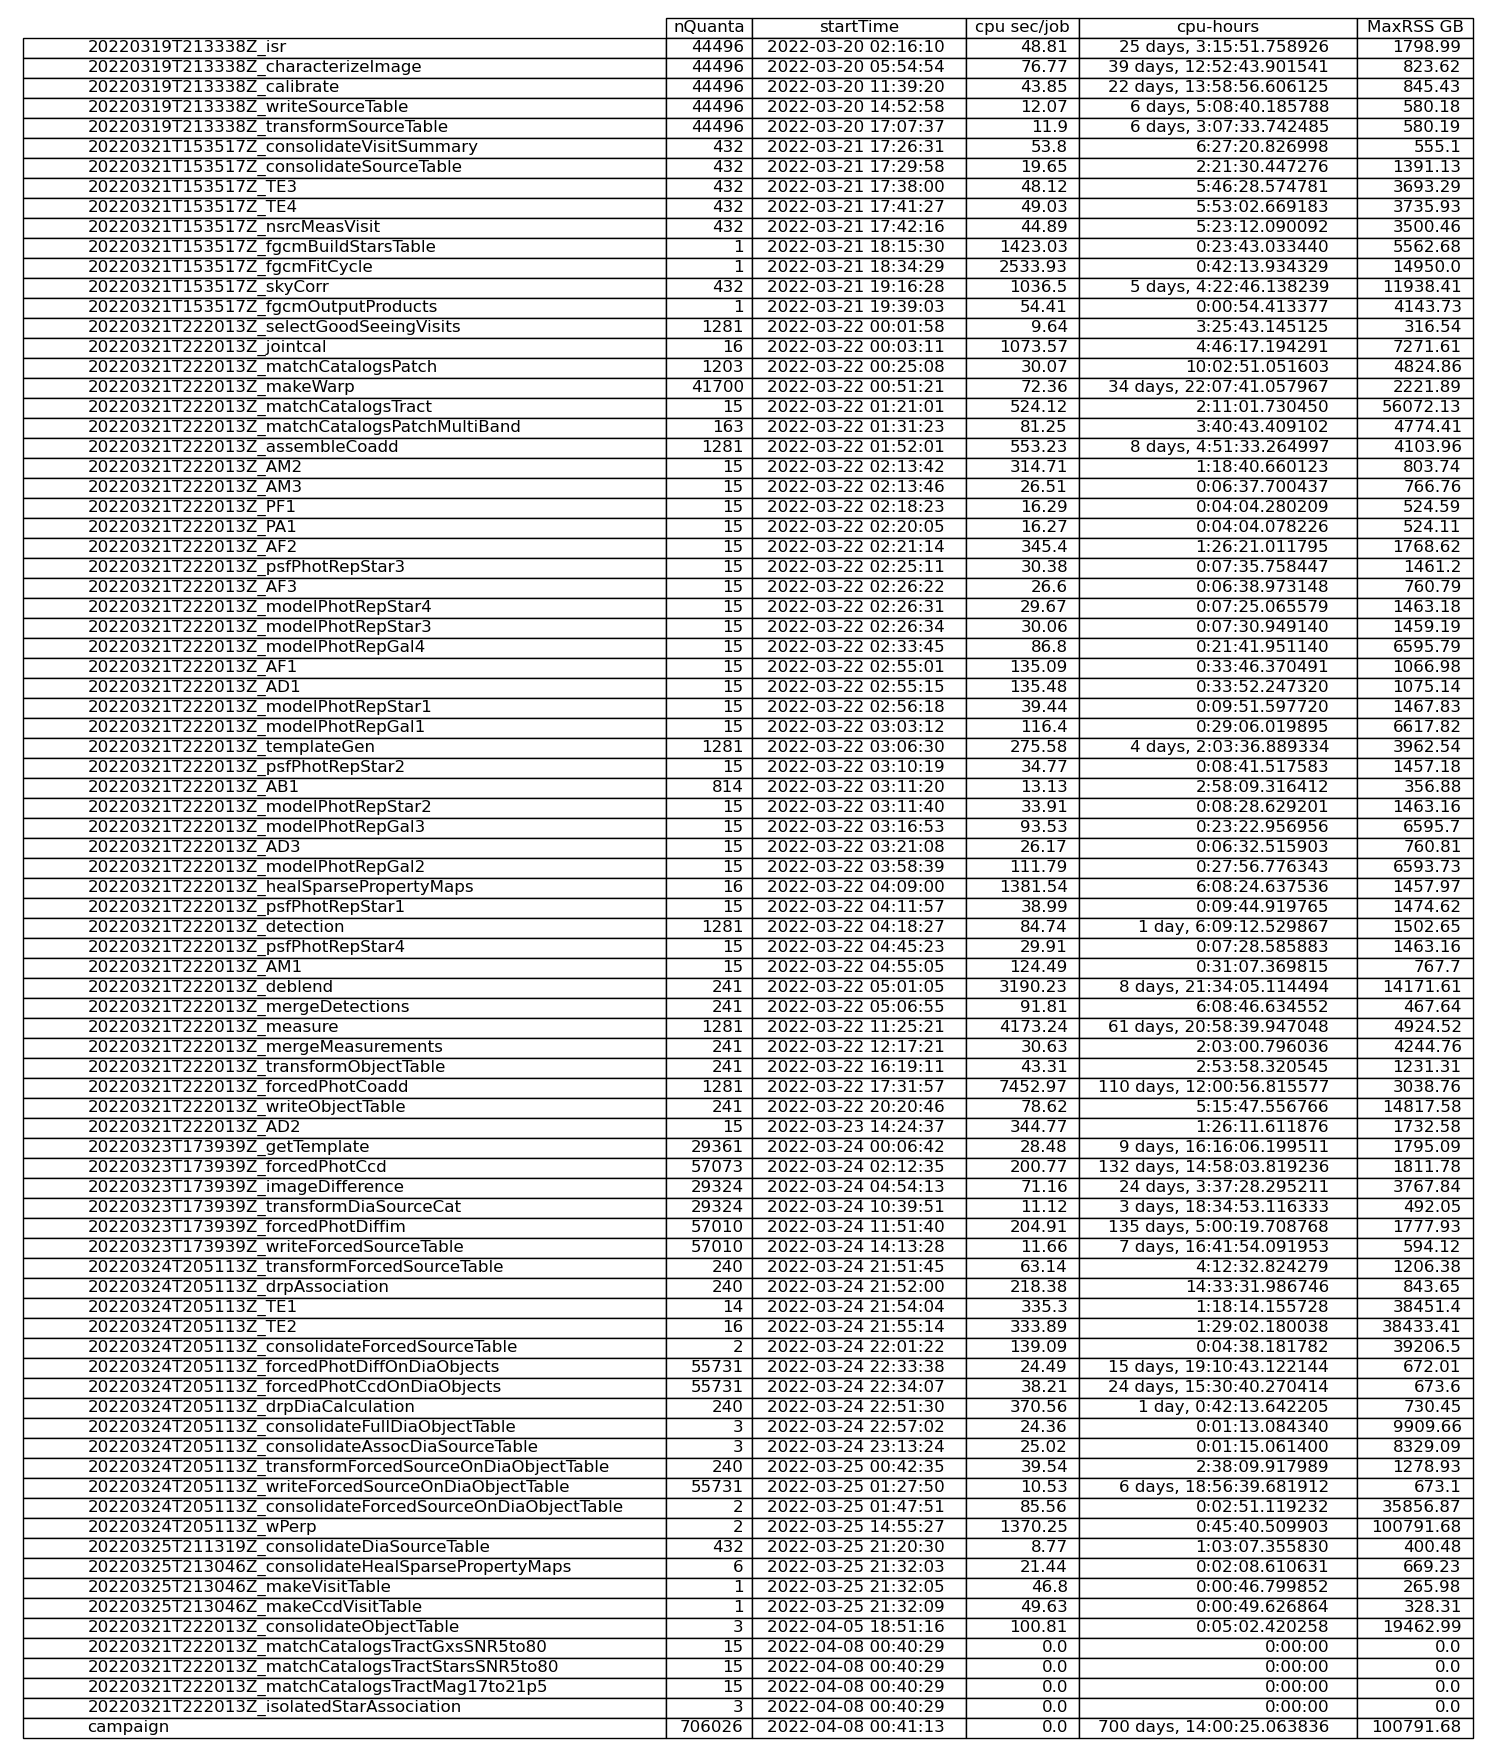
\includegraphics[width=5.96875in]{jira_imgs/2294.png}

}


\subsection{Test Cycle LVV-C162 }

Open test cycle {\it \href{https://jira.lsstcorp.org/secure/Tests.jspa#/testrun/LVV-C162}{LDM-503-GEN3: Gen 3 Ingest raw dataset}} in Jira.

Test Cycle name: LDM-503-GEN3: Gen 3 Ingest raw dataset\\
Status: Not Executed

In the context of the milestone LDM-503-GEN3, Gen 3 Butler readiness,
this test cycle is defining the configuration and the dataset for
running a generic \textbf{Raw Data Ingestion Into Gen3 Butler} test
case. ~ There are currently 5 data sources that require verification as
they are the central products that will be produced by Rubin or are used
as precursor sets in the development/verification of the data management
software systems. ~The current raw data products that are deemed central
to DM development and testing are those from AuxTel/LATISS, ComCam, and
~precursor data from HyperSuprimeCam (HSC). ~Note, further tests using
LSSTCam (currently only preliminary BOT data from the SLAC test stand
are available) or precursor sets from the Dark Energy Camera (DECam)
could be added but since these types do not exactly fit the central
model used for LSST they are not tied directly to requirements.

\subsubsection{Software Version/Baseline}
LSST DM Stack with Gen3 Butler.

\subsubsection{Configuration}
Three separate raw data types, those from: AuxTel/LATISS, ComCam, and
HSC (e.g. a CI\_HSC raw) should be ingested when this test is executed.

\subsubsection{Test Cases in LVV-C162 Test Cycle}

\paragraph{ LVV-T1985 - Verify daf\_butler raw data ingest }\mbox{}\\

Version \textbf{1}.
Open  \href{https://jira.lsstcorp.org/secure/Tests.jspa#/testCase/LVV-T1985}{\textit{ LVV-T1985 } }
test case in Jira.

Demonstrate that a raw data type can be successfully ingested into a
Butler repository. ~

\textbf{ Preconditions}:\\
In order to run this test, a Gen3 daf butler should be deployed and
ready to use, with access to the filesystems where the raw data to
ingest is stored.

Execution status: {\bf Not Executed }

Final comment:\\


Detailed steps results:

\begin{tabular}{p{2cm}p{14cm}}
\toprule
Step 1 & Step Execution Status: \textbf{ Not Executed } \\ \hline
\end{tabular}
 Description \\
{\footnotesize
Identify data for ingestion~{HSC RC2}⁠ and make ~a copy at a location
for the test. ~While a suggestion is provided in
{/project/shared/hsc/COSMOS/2014-03-27/}⁠ for a location where such data
can be found, the actual data used can be left to the discretion of the
person(s) executing the test with the added suggestion that relatively
recent data are more likely to reflect the current observatory system
state.\\[2\baselineskip]

}
\hdashrule[0.5ex]{\textwidth}{1pt}{3mm}
  Test Data \\
 {\footnotesize
{/project/shared/hsc/COSMOS/2014-03-27/}⁠~⁠~

}
\hdashrule[0.5ex]{\textwidth}{1pt}{3mm}
  Expected Result \\
{\footnotesize
One or more raw data sets are identified and made available.

}
\hdashrule[0.5ex]{\textwidth}{1pt}{3mm}
  Actual Result \\
{\footnotesize

}
\begin{tabular}{p{2cm}p{14cm}}
\toprule
Step 2 & Step Execution Status: \textbf{ Not Executed } \\ \hline
\end{tabular}
 Description \\
{\footnotesize
Identify data for ingestion~{AuxTel/LATISS}⁠ and make ~a copy at a
location for the test. ~While a suggestion is provided in
{/project/shared/auxTel/\_parent/raw/2021-03-23/}⁠ for a location where
such data can be found, the actual data used can be left to the
discretion of the person(s) executing the test with the added suggestion
that relatively recent data are more likely to reflect the current
observatory system state.\\[2\baselineskip]

}
\hdashrule[0.5ex]{\textwidth}{1pt}{3mm}
  Test Data \\
 {\footnotesize
{/project/shared/auxTel/\_parent/raw/2021-03-23/}⁠~⁠~

}
\hdashrule[0.5ex]{\textwidth}{1pt}{3mm}
  Expected Result \\
{\footnotesize
One or more raw data sets are identified and made available.

}
\hdashrule[0.5ex]{\textwidth}{1pt}{3mm}
  Actual Result \\
{\footnotesize

}
\begin{tabular}{p{2cm}p{14cm}}
\toprule
Step 3 & Step Execution Status: \textbf{ Not Executed } \\ \hline
\end{tabular}
 Description \\
{\footnotesize
Identify data for ingestion~{ComCam}⁠ and make ~a copy at a location for
the test. ~While a suggestion is provided in
{/project/shared/comCam/\_parent/raw/2021-05-14/2021051400003/}⁠ for a
location where such data can be found, the actual data used can be left
to the discretion of the person(s) executing the test with the added
suggestion that relatively recent data are more likely to reflect the
current observatory system state.\\[2\baselineskip]

}
\hdashrule[0.5ex]{\textwidth}{1pt}{3mm}
  Test Data \\
 {\footnotesize
{/project/shared/comCam/\_parent/raw/2021-05-14/2021051400003/}⁠~⁠~

}
\hdashrule[0.5ex]{\textwidth}{1pt}{3mm}
  Expected Result \\
{\footnotesize
One or more raw data sets are identified and made available.

}
\hdashrule[0.5ex]{\textwidth}{1pt}{3mm}
  Actual Result \\
{\footnotesize

}
\begin{tabular}{p{2cm}p{14cm}}
\toprule
Step 4 & Step Execution Status: \textbf{ Not Executed } \\ \hline
\end{tabular}
 Description \\
{\footnotesize
Verify that Butler repository is available for the {HSC RC2}⁠ (Note this
needs to be a test repository rather than the central repository as the
raw data should not already be present in the repository for this test.)

}
\hdashrule[0.5ex]{\textwidth}{1pt}{3mm}
  Test Data \\
 {\footnotesize
{url 1}⁠~

}
\hdashrule[0.5ex]{\textwidth}{1pt}{3mm}
  Example Code \\
{\footnotesize
\# create empty Gen3 repo (for ComCam data)\\[2\baselineskip]butler
create repo\\
butler register-instrument repo lsst.obs.lsst.LsstComCam

}
\hdashrule[0.5ex]{\textwidth}{1pt}{3mm}
  Expected Result \\
{\footnotesize

}
\hdashrule[0.5ex]{\textwidth}{1pt}{3mm}
  Actual Result \\
{\footnotesize

}
\begin{tabular}{p{2cm}p{14cm}}
\toprule
Step 5 & Step Execution Status: \textbf{ Not Executed } \\ \hline
\end{tabular}
 Description \\
{\footnotesize
Verify that Butler repository is available for the {AuxTel/LATISS}⁠
(Note this needs to be a test repository rather than the central
repository as the raw data should not already be present in the
repository for this test.)

}
\hdashrule[0.5ex]{\textwidth}{1pt}{3mm}
  Test Data \\
 {\footnotesize
{url 2}⁠~

}
\hdashrule[0.5ex]{\textwidth}{1pt}{3mm}
  Example Code \\
{\footnotesize
\# create empty Gen3 repo (for ComCam data)\\[2\baselineskip]butler
create repo\\
butler register-instrument repo lsst.obs.lsst.LsstComCam

}
\hdashrule[0.5ex]{\textwidth}{1pt}{3mm}
  Expected Result \\
{\footnotesize

}
\hdashrule[0.5ex]{\textwidth}{1pt}{3mm}
  Actual Result \\
{\footnotesize

}
\begin{tabular}{p{2cm}p{14cm}}
\toprule
Step 6 & Step Execution Status: \textbf{ Not Executed } \\ \hline
\end{tabular}
 Description \\
{\footnotesize
Verify that Butler repository is available for the {ComCam}⁠ (Note this
needs to be a test repository rather than the central repository as the
raw data should not already be present in the repository for this test.)

}
\hdashrule[0.5ex]{\textwidth}{1pt}{3mm}
  Test Data \\
 {\footnotesize
{url 3}⁠~

}
\hdashrule[0.5ex]{\textwidth}{1pt}{3mm}
  Example Code \\
{\footnotesize
\# create empty Gen3 repo (for ComCam data)\\[2\baselineskip]butler
create repo\\
butler register-instrument repo lsst.obs.lsst.LsstComCam

}
\hdashrule[0.5ex]{\textwidth}{1pt}{3mm}
  Expected Result \\
{\footnotesize

}
\hdashrule[0.5ex]{\textwidth}{1pt}{3mm}
  Actual Result \\
{\footnotesize

}
\begin{tabular}{p{2cm}p{14cm}}
\toprule
Step 7 & Step Execution Status: \textbf{ Not Executed } \\ \hline
\end{tabular}
 Description \\
{\footnotesize
Ingest {HSC RC2}⁠~raw data into repo

}
\hdashrule[0.5ex]{\textwidth}{1pt}{3mm}
  Test Data \\
 {\footnotesize
{url 1}⁠~

}
\hdashrule[0.5ex]{\textwidth}{1pt}{3mm}
  Example Code \\
{\footnotesize
butler ingest-raws repo raw

}
\hdashrule[0.5ex]{\textwidth}{1pt}{3mm}
  Expected Result \\
{\footnotesize
Tool reports data ingest successful for {HSC RC2}⁠ into {url 1}⁠~

}
\hdashrule[0.5ex]{\textwidth}{1pt}{3mm}
  Actual Result \\
{\footnotesize

}
\begin{tabular}{p{2cm}p{14cm}}
\toprule
Step 8 & Step Execution Status: \textbf{ Not Executed } \\ \hline
\end{tabular}
 Description \\
{\footnotesize
Ingest {AuxTel/LATISS}⁠~raw data into repo

}
\hdashrule[0.5ex]{\textwidth}{1pt}{3mm}
  Test Data \\
 {\footnotesize
{url 2}⁠~

}
\hdashrule[0.5ex]{\textwidth}{1pt}{3mm}
  Example Code \\
{\footnotesize
butler ingest-raws repo raw

}
\hdashrule[0.5ex]{\textwidth}{1pt}{3mm}
  Expected Result \\
{\footnotesize
Tool reports data ingest successful for {AuxTel/LATISS}⁠ into {url 2}⁠~

}
\hdashrule[0.5ex]{\textwidth}{1pt}{3mm}
  Actual Result \\
{\footnotesize

}
\begin{tabular}{p{2cm}p{14cm}}
\toprule
Step 9 & Step Execution Status: \textbf{ Not Executed } \\ \hline
\end{tabular}
 Description \\
{\footnotesize
Ingest {ComCam}⁠~raw data into repo

}
\hdashrule[0.5ex]{\textwidth}{1pt}{3mm}
  Test Data \\
 {\footnotesize
{url 3}⁠~

}
\hdashrule[0.5ex]{\textwidth}{1pt}{3mm}
  Example Code \\
{\footnotesize
butler ingest-raws repo raw

}
\hdashrule[0.5ex]{\textwidth}{1pt}{3mm}
  Expected Result \\
{\footnotesize
Tool reports data ingest successful for {ComCam}⁠ into {url 3}⁠~

}
\hdashrule[0.5ex]{\textwidth}{1pt}{3mm}
  Actual Result \\
{\footnotesize

}
\begin{tabular}{p{2cm}p{14cm}}
\toprule
Step 10 & Step Execution Status: \textbf{ Not Executed } \\ \hline
\end{tabular}
 Description \\
{\footnotesize
Query repository to verify that ingestion of {HSC RC2}⁠~ occurred.

}
\hdashrule[0.5ex]{\textwidth}{1pt}{3mm}
  Test Data \\
 {\footnotesize
{url 1}⁠~

}
\hdashrule[0.5ex]{\textwidth}{1pt}{3mm}
  Expected Result \\
{\footnotesize
{HSC RC2}⁠ data are found by query.~

}
\hdashrule[0.5ex]{\textwidth}{1pt}{3mm}
  Actual Result \\
{\footnotesize

}
\begin{tabular}{p{2cm}p{14cm}}
\toprule
Step 11 & Step Execution Status: \textbf{ Not Executed } \\ \hline
\end{tabular}
 Description \\
{\footnotesize
Query repository to verify that ingestion of {AuxTel/LATISS}⁠~ occurred.

}
\hdashrule[0.5ex]{\textwidth}{1pt}{3mm}
  Test Data \\
 {\footnotesize
{url 2}⁠~

}
\hdashrule[0.5ex]{\textwidth}{1pt}{3mm}
  Expected Result \\
{\footnotesize
{AuxTel/LATISS}⁠ data are found by query.~

}
\hdashrule[0.5ex]{\textwidth}{1pt}{3mm}
  Actual Result \\
{\footnotesize

}
\begin{tabular}{p{2cm}p{14cm}}
\toprule
Step 12 & Step Execution Status: \textbf{ Not Executed } \\ \hline
\end{tabular}
 Description \\
{\footnotesize
Query repository to verify that ingestion of {ComCam}⁠~ occurred.

}
\hdashrule[0.5ex]{\textwidth}{1pt}{3mm}
  Test Data \\
 {\footnotesize
{url 3}⁠~

}
\hdashrule[0.5ex]{\textwidth}{1pt}{3mm}
  Expected Result \\
{\footnotesize
{ComCam}⁠ data are found by query.~

}
\hdashrule[0.5ex]{\textwidth}{1pt}{3mm}
  Actual Result \\
{\footnotesize

}


\subsection{Test Cycle LVV-C190 }

Open test cycle {\it \href{https://jira.lsstcorp.org/secure/Tests.jspa#/testrun/LVV-C190}{\citeds{LDM-556}: Middleware Acceptance Testing}} in Jira.

Test Cycle name: \citeds{LDM-556}: Middleware Acceptance Testing\\
Status: In Progress



\subsubsection{Software Version/Baseline}
Not provided.

\subsubsection{Configuration}
Not provided.

\subsubsection{Test Cases in LVV-C190 Test Cycle}

\paragraph{ LVV-T2503 - Verify Outputs from Test Processing Runs }\mbox{}\\

Version \textbf{1}.
Open  \href{https://jira.lsstcorp.org/secure/Tests.jspa#/testCase/LVV-T2503}{\textit{ LVV-T2503 } }
test case in Jira.

Verify that the Data Output System interface is usable by algorithmic
code being run for test/development purposes, on both development
compute environments at the archive center and in personal environments.

\textbf{ Preconditions}:\\


Execution status: {\bf Not Executed }

Final comment:\\


Detailed steps results:

\begin{tabular}{p{2cm}p{14cm}}
\toprule
Step 1 & Step Execution Status: \textbf{ Not Executed } \\ \hline
\end{tabular}
 Description \\
{\footnotesize
Demonstrated by regular reprocessing runs at NCSA.

}
\hdashrule[0.5ex]{\textwidth}{1pt}{3mm}
  Expected Result \\
{\footnotesize

}
\hdashrule[0.5ex]{\textwidth}{1pt}{3mm}
  Actual Result \\
{\footnotesize

}

\paragraph{ LVV-T2502 - Verify Outputs from Science Platform }\mbox{}\\

Version \textbf{1}.
Open  \href{https://jira.lsstcorp.org/secure/Tests.jspa#/testCase/LVV-T2502}{\textit{ LVV-T2502 } }
test case in Jira.

Verify that the ~Data Output System interface shall be usable by
algorithmic code run in the Science Platform

\textbf{ Preconditions}:\\


Execution status: {\bf Not Executed }

Final comment:\\


Detailed steps results:

\begin{tabular}{p{2cm}p{14cm}}
\toprule
Step 1 & Step Execution Status: \textbf{ Not Executed } \\ \hline
\end{tabular}
 Description \\
{\footnotesize
Demonstrated by any Science Platform notebook that uses the butler.

}
\hdashrule[0.5ex]{\textwidth}{1pt}{3mm}
  Expected Result \\
{\footnotesize

}
\hdashrule[0.5ex]{\textwidth}{1pt}{3mm}
  Actual Result \\
{\footnotesize

}

\paragraph{ LVV-T2501 - Verify Outputs from Data Release Production }\mbox{}\\

Version \textbf{1}.
Open  \href{https://jira.lsstcorp.org/secure/Tests.jspa#/testCase/LVV-T2501}{\textit{ LVV-T2501 } }
test case in Jira.

Verify that the Data Output System interface is usable by algorithmic
code being run as part of Data Release
Production.\\[2\baselineskip]Demonstrated by regular reprocessing runs
at NCSA and DP0.2 production.

\textbf{ Preconditions}:\\


Execution status: {\bf Not Executed }

Final comment:\\


Detailed steps results:

\begin{tabular}{p{2cm}p{14cm}}
\toprule
Step 1 & Step Execution Status: \textbf{ Not Executed } \\ \hline
\end{tabular}
 Description \\
{\footnotesize

}
\hdashrule[0.5ex]{\textwidth}{1pt}{3mm}
  Expected Result \\
{\footnotesize

}
\hdashrule[0.5ex]{\textwidth}{1pt}{3mm}
  Actual Result \\
{\footnotesize

}

\paragraph{ LVV-T2499 - Verify Consistent Output Interface }\mbox{}\\

Version \textbf{1}.
Open  \href{https://jira.lsstcorp.org/secure/Tests.jspa#/testCase/LVV-T2499}{\textit{ LVV-T2499 } }
test case in Jira.

Verify that the ~Data Output System ~provides a consistent interface for
writing InMemoryDatasets to storage given a DatasetRef across different
types of DataRepositories.

\textbf{ Preconditions}:\\


Execution status: {\bf Not Executed }

Final comment:\\


Detailed steps results:

\begin{tabular}{p{2cm}p{14cm}}
\toprule
Step 1 & Step Execution Status: \textbf{ Not Executed } \\ \hline
\end{tabular}
 Description \\
{\footnotesize

}
\hdashrule[0.5ex]{\textwidth}{1pt}{3mm}
  Expected Result \\
{\footnotesize

}
\hdashrule[0.5ex]{\textwidth}{1pt}{3mm}
  Actual Result \\
{\footnotesize

}

\paragraph{ LVV-T2498 - Verify Writing FITS tables }\mbox{}\\

Version \textbf{1}.
Open  \href{https://jira.lsstcorp.org/secure/Tests.jspa#/testCase/LVV-T2498}{\textit{ LVV-T2498 } }
test case in Jira.

Verify that the Data Output System is able to write in-memory table
objects as FITS files.

\textbf{ Preconditions}:\\


Execution status: {\bf Pass }

Final comment:\\


Detailed steps results:

\begin{tabular}{p{2cm}p{14cm}}
\toprule
Step 1 & Step Execution Status: \textbf{ Pass } \\ \hline
\end{tabular}
 Description \\
{\footnotesize
Execute unit tests ``test\_fitsTables.cc'' and ``test\_fits.py'' in
\href{https://github.com/lsst/afw}{lsst.afw} package.

}
\hdashrule[0.5ex]{\textwidth}{1pt}{3mm}
  Expected Result \\
{\footnotesize
Unit tests pass.

}
\hdashrule[0.5ex]{\textwidth}{1pt}{3mm}
  Actual Result \\
{\footnotesize
Executed `scons` in a cloned version of the `afw` package on lsst-devl
at NCSA. Here is the relevant line from the log indicating that the C++
unit tests in ``test\_fitsTables.cc'' passed:\\[2\baselineskip]running
tests/test\_fitsTables\ldots{} passed\\[2\baselineskip]Next, execute the
`test\_fits.py` unit test on its own:\\[2\baselineskip]pytest -s -vv
--no-header --cache-clear
tests/test\_fits.py\\[2\baselineskip]Results:\\[2\baselineskip]tests/test\_fits.py::FLAKE8
PASSED\\
tests/test\_fits.py::FitsTestCase::testIgnoreKeywords~PASSED\\
tests/test\_fits.py::FitsTestCase::testReadBlankKeywordComment~PASSED\\
tests/test\_fits.py::FitsTestCase::testReadUndefined lsst.afw.fits WARN:
In void
lsst::afw::fits::\{anonymous\}::MetadataIterationFunctor::add(const
string\&, const string\&), dropping undefined value for key `ADC-STR'.\\
lsst.afw.fits WARN: In void
lsst::afw::fits::\{anonymous\}::MetadataIterationFunctor::add(const
string\&, T, const string\&) {[}with T = double; std::string =
std::\_\_cxx11::basic\_string\textless{}char\textgreater{}{]}, replacing
undefined value for key `DOM-WND'.\\
PASSED\\
tests/test\_fits.py::FitsTestCase::testSimpleIO~PASSED\\
tests/test\_fits.py::FitsTestCase::testUndefinedVector~PASSED\\
tests/test\_fits.py::TestMemory::testFileDescriptorLeaks \textless{}-
../../../../../software/lsstsw/stack\_20220215/stack/miniconda3-py38\_4.9.2-2.0.0/Linux64/utils/g617c0b0dc2+9633a190c8/python/lsst/utils/tests.py
PASSED\\[2\baselineskip]Thus the writing of FITS tables has been
demonstrated.

}

\paragraph{ LVV-T2497 - Verify Writing FITS images }\mbox{}\\

Version \textbf{1}.
Open  \href{https://jira.lsstcorp.org/secure/Tests.jspa#/testCase/LVV-T2497}{\textit{ LVV-T2497 } }
test case in Jira.

Verify that the ~Data Output System is able to write in-memory image
objects as FITS files

\textbf{ Preconditions}:\\


Execution status: {\bf Pass }

Final comment:\\


Detailed steps results:

\begin{tabular}{p{2cm}p{14cm}}
\toprule
Step 1 & Step Execution Status: \textbf{ Pass } \\ \hline
\end{tabular}
 Description \\
{\footnotesize
Execute unit tests ``test\_imageIo1.py'' and ``test\_imageIo2.py'' in
\href{https://github.com/lsst/afw}{lsst.afw}~package.

}
\hdashrule[0.5ex]{\textwidth}{1pt}{3mm}
  Expected Result \\
{\footnotesize
Unit tests pass.

}
\hdashrule[0.5ex]{\textwidth}{1pt}{3mm}
  Actual Result \\
{\footnotesize
First, clone and set up the `afwdata` package:\\
git clone https://github.com/lsst/afwdata.git\\
cd afwdata\\
setup -j -r .\\[2\baselineskip]Now navigate to a cloned, set up
repository of `lsst.afw` on the lsst-devl machines at NCSA, and execute
the following:\\[2\baselineskip]pytest -s -vv --no-header --cache-clear
tests/test\_imageIo1.py\\[2\baselineskip]Results:\\
tests/test\_imageIo1.py::FLAKE8~PASSED\\
tests/test\_imageIo1.py::ReadFitsTestCase::testBBoxFromMetadata~PASSED\\
tests/test\_imageIo1.py::ReadFitsTestCase::testF32~PASSED\\
tests/test\_imageIo1.py::ReadFitsTestCase::testF64~PASSED\\
tests/test\_imageIo1.py::ReadFitsTestCase::testImageCompressionDisabled~PASSED\\
tests/test\_imageIo1.py::ReadFitsTestCase::testLongStrings~PASSED\\
tests/test\_imageIo1.py::ReadFitsTestCase::testMEF~PASSED\\
tests/test\_imageIo1.py::ReadFitsTestCase::testReadFitsWithOptions~PASSED\\
tests/test\_imageIo1.py::ReadFitsTestCase::testS16~PASSED\\
tests/test\_imageIo1.py::ReadFitsTestCase::testSubimage~PASSED\\
tests/test\_imageIo1.py::ReadFitsTestCase::testU16~PASSED\\
tests/test\_imageIo1.py::ReadFitsTestCase::testWriteBool~PASSED\\
tests/test\_imageIo1.py::ReadFitsTestCase::testWriteReadF64~PASSED\\
tests/test\_imageIo1.py::TestMemory::testFileDescriptorLeaks
\textless{}-
../../../../../software/lsstsw/stack\_20220215/stack/miniconda3-py38\_4.9.2-2.0.0/Linux64/utils/g617c0b0dc2+9633a190c8/python/lsst/utils/tests.py
PASSED\\[2\baselineskip]pytest -s -vv --no-header --cache-clear
tests/test\_imageIo2.py\\[2\baselineskip]Results:\\
tests/test\_imageIo2.py::FLAKE8~PASSED\\
tests/test\_imageIo2.py::ImageIoTestCase::testFloatCompressedLossless~PASSED\\
tests/test\_imageIo2.py::ImageIoTestCase::testFloatCompressedManual~SKIPPED~(Fix
deferred to DM-15644)\\
tests/test\_imageIo2.py::ImageIoTestCase::testFloatCompressedRange~SKIPPED~(Fix
deferred to DM-15644)\\
tests/test\_imageIo2.py::ImageIoTestCase::testFloatUncompressed~PASSED\\
tests/test\_imageIo2.py::ImageIoTestCase::testIntegerCompression~PASSED\\
tests/test\_imageIo2.py::ImageIoTestCase::testIntegerUncompression~PASSED\\
tests/test\_imageIo2.py::ImageIoTestCase::testUInt64~PASSED\\
tests/test\_imageIo2.py::TestMemory::testFileDescriptorLeaks
\textless{}-
../../../../../software/lsstsw/stack\_20220215/stack/miniconda3-py38\_4.9.2-2.0.0/Linux64/utils/g617c0b0dc2+9633a190c8/python/lsst/utils/tests.py
P\\[2\baselineskip]We have now demonstrated the reading and writing of
FITS images.

}

\paragraph{ LVV-T2496 - Verify filename invariance }\mbox{}\\

Version \textbf{1}.
Open  \href{https://jira.lsstcorp.org/secure/Tests.jspa#/testCase/LVV-T2496}{\textit{ LVV-T2496 } }
test case in Jira.

Verify that for all datasets stored with unique filenames (or paths) as
part of a Data Release, the name of the file retrieved by an external
user is also unique and has a predictable name that is not dependent on
data access mechanism\\[2\baselineskip]This behavior is not guaranteed
by code, but it is the way we have configured our filename templates.

\textbf{ Preconditions}:\\


Execution status: {\bf Not Executed }

Final comment:\\


Detailed steps results:

\begin{tabular}{p{2cm}p{14cm}}
\toprule
Step 1 & Step Execution Status: \textbf{ Not Executed } \\ \hline
\end{tabular}
 Description \\
{\footnotesize

}
\hdashrule[0.5ex]{\textwidth}{1pt}{3mm}
  Expected Result \\
{\footnotesize

}
\hdashrule[0.5ex]{\textwidth}{1pt}{3mm}
  Actual Result \\
{\footnotesize

}

\paragraph{ LVV-T2495 - Verify Combining composite datasets for export }\mbox{}\\

Version \textbf{1}.
Open  \href{https://jira.lsstcorp.org/secure/Tests.jspa#/testCase/LVV-T2495}{\textit{ LVV-T2495 } }
test case in Jira.

Verify that a facility is available to combine file-based composite
datasets into a single file in a Scientific Data Format

\textbf{ Preconditions}:\\


Execution status: {\bf Not Executed }

Final comment:\\


Detailed steps results:

\begin{tabular}{p{2cm}p{14cm}}
\toprule
Step 1 & Step Execution Status: \textbf{ Not Executed } \\ \hline
\end{tabular}
 Description \\
{\footnotesize

}
\hdashrule[0.5ex]{\textwidth}{1pt}{3mm}
  Expected Result \\
{\footnotesize

}
\hdashrule[0.5ex]{\textwidth}{1pt}{3mm}
  Actual Result \\
{\footnotesize

}

\paragraph{ LVV-T2494 - Verify Strong exception guarantee }\mbox{}\\

Version \textbf{1}.
Open  \href{https://jira.lsstcorp.org/secure/Tests.jspa#/testCase/LVV-T2494}{\textit{ LVV-T2494 } }
test case in Jira.

Verify that a put operation on the Data Output System ~provides the
strong exception guarantee. If a put operation fails the previous state
shall be restored.\\[2\baselineskip]This is the usual behavior, and we
regard it as a bug when it is violated, and we don't currently have any
known bugs of this type.

\textbf{ Preconditions}:\\


Execution status: {\bf Not Executed }

Final comment:\\


Detailed steps results:

\begin{tabular}{p{2cm}p{14cm}}
\toprule
Step 1 & Step Execution Status: \textbf{ Not Executed } \\ \hline
\end{tabular}
 Description \\
{\footnotesize

}
\hdashrule[0.5ex]{\textwidth}{1pt}{3mm}
  Expected Result \\
{\footnotesize

}
\hdashrule[0.5ex]{\textwidth}{1pt}{3mm}
  Actual Result \\
{\footnotesize

}

\paragraph{ LVV-T2493 - Verify No clobber }\mbox{}\\

Version \textbf{1}.
Open  \href{https://jira.lsstcorp.org/secure/Tests.jspa#/testCase/LVV-T2493}{\textit{ LVV-T2493 } }
test case in Jira.

Verify that it is possible to configure the Data Output System such that
it is an error to attempt to persist a dataset that is already present
in the output repository

\textbf{ Preconditions}:\\


Execution status: {\bf Not Executed }

Final comment:\\


Detailed steps results:

\begin{tabular}{p{2cm}p{14cm}}
\toprule
Step 1 & Step Execution Status: \textbf{ Not Executed } \\ \hline
\end{tabular}
 Description \\
{\footnotesize

}
\hdashrule[0.5ex]{\textwidth}{1pt}{3mm}
  Expected Result \\
{\footnotesize

}
\hdashrule[0.5ex]{\textwidth}{1pt}{3mm}
  Actual Result \\
{\footnotesize

}

\paragraph{ LVV-T2492 - Verify Blocked write operation }\mbox{}\\

Version \textbf{1}.
Open  \href{https://jira.lsstcorp.org/secure/Tests.jspa#/testCase/LVV-T2492}{\textit{ LVV-T2492 } }
test case in Jira.

Verify that a put operation on the Data Output System blocks until it
has either worked or failed

\textbf{ Preconditions}:\\


Execution status: {\bf Not Executed }

Final comment:\\


Detailed steps results:

\begin{tabular}{p{2cm}p{14cm}}
\toprule
Step 1 & Step Execution Status: \textbf{ Not Executed } \\ \hline
\end{tabular}
 Description \\
{\footnotesize

}
\hdashrule[0.5ex]{\textwidth}{1pt}{3mm}
  Expected Result \\
{\footnotesize

}
\hdashrule[0.5ex]{\textwidth}{1pt}{3mm}
  Actual Result \\
{\footnotesize

}

\paragraph{ LVV-T2491 - Verify Creation of new DatasetTypes }\mbox{}\\

Version \textbf{1}.
Open  \href{https://jira.lsstcorp.org/secure/Tests.jspa#/testCase/LVV-T2491}{\textit{ LVV-T2491 } }
test case in Jira.

Verify that the Data Output system ~allows a new DatasetType to be
registered with a DataRepository, programmatically and at Supertask
preflight-time, allowing Datasets of that DatasetType to be added to
that DataRepository thereafter

\textbf{ Preconditions}:\\


Execution status: {\bf Not Executed }

Final comment:\\


Detailed steps results:

\begin{tabular}{p{2cm}p{14cm}}
\toprule
Step 1 & Step Execution Status: \textbf{ Not Executed } \\ \hline
\end{tabular}
 Description \\
{\footnotesize

}
\hdashrule[0.5ex]{\textwidth}{1pt}{3mm}
  Expected Result \\
{\footnotesize

}
\hdashrule[0.5ex]{\textwidth}{1pt}{3mm}
  Actual Result \\
{\footnotesize

}

\paragraph{ LVV-T2488 - Verify access outputs from test processing runs }\mbox{}\\

Version \textbf{1}.
Open  \href{https://jira.lsstcorp.org/secure/Tests.jspa#/testCase/LVV-T2488}{\textit{ LVV-T2488 } }
test case in Jira.

Verify that the Data Input System shall provide access to processing
runs initiated for test/development purposes, from the same compute
environment in which the processing was run

\textbf{ Preconditions}:\\


Execution status: {\bf Not Executed }

Final comment:\\


Detailed steps results:

\begin{tabular}{p{2cm}p{14cm}}
\toprule
Step 1 & Step Execution Status: \textbf{ Not Executed } \\ \hline
\end{tabular}
 Description \\
{\footnotesize
Instantiate a Butler at NCSA or SLAC targeting a test run in
`/repo/main`.

}
\hdashrule[0.5ex]{\textwidth}{1pt}{3mm}
  Expected Result \\
{\footnotesize

}
\hdashrule[0.5ex]{\textwidth}{1pt}{3mm}
  Actual Result \\
{\footnotesize

}
\begin{tabular}{p{2cm}p{14cm}}
\toprule
Step 2 & Step Execution Status: \textbf{ Not Executed } \\ \hline
\end{tabular}
 Description \\
{\footnotesize
Call Butler.get.

}
\hdashrule[0.5ex]{\textwidth}{1pt}{3mm}
  Expected Result \\
{\footnotesize

}
\hdashrule[0.5ex]{\textwidth}{1pt}{3mm}
  Actual Result \\
{\footnotesize

}
\begin{tabular}{p{2cm}p{14cm}}
\toprule
Step 3 & Step Execution Status: \textbf{ Not Executed } \\ \hline
\end{tabular}
 Description \\
{\footnotesize
Verify that data is correctly retrieved

}
\hdashrule[0.5ex]{\textwidth}{1pt}{3mm}
  Expected Result \\
{\footnotesize

}
\hdashrule[0.5ex]{\textwidth}{1pt}{3mm}
  Actual Result \\
{\footnotesize

}

\paragraph{ LVV-T2487 - Verify Accessing official Data Releases }\mbox{}\\

Version \textbf{1}.
Open  \href{https://jira.lsstcorp.org/secure/Tests.jspa#/testCase/LVV-T2487}{\textit{ LVV-T2487 } }
test case in Jira.

Verify that the ~Data Input System interface shall provide access to
official Data Releases from the LSST Science Platform.

\textbf{ Preconditions}:\\


Execution status: {\bf Not Executed }

Final comment:\\


Detailed steps results:

\begin{tabular}{p{2cm}p{14cm}}
\toprule
Step 1 & Step Execution Status: \textbf{ Not Executed } \\ \hline
\end{tabular}
 Description \\
{\footnotesize
Instantiate a butler on RSP targeting DP0.x
collections.\\[2\baselineskip]

}
\hdashrule[0.5ex]{\textwidth}{1pt}{3mm}
  Expected Result \\
{\footnotesize

}
\hdashrule[0.5ex]{\textwidth}{1pt}{3mm}
  Actual Result \\
{\footnotesize

}
\begin{tabular}{p{2cm}p{14cm}}
\toprule
Step 2 & Step Execution Status: \textbf{ Not Executed } \\ \hline
\end{tabular}
 Description \\
{\footnotesize
Call `Butler.get`~

}
\hdashrule[0.5ex]{\textwidth}{1pt}{3mm}
  Expected Result \\
{\footnotesize

}
\hdashrule[0.5ex]{\textwidth}{1pt}{3mm}
  Actual Result \\
{\footnotesize

}
\begin{tabular}{p{2cm}p{14cm}}
\toprule
Step 3 & Step Execution Status: \textbf{ Not Executed } \\ \hline
\end{tabular}
 Description \\
{\footnotesize
Verify that data is retrieved

}
\hdashrule[0.5ex]{\textwidth}{1pt}{3mm}
  Expected Result \\
{\footnotesize

}
\hdashrule[0.5ex]{\textwidth}{1pt}{3mm}
  Actual Result \\
{\footnotesize

}

\paragraph{ LVV-T2486 - Verify Consistent input interface }\mbox{}\\

Version \textbf{1}.
Open  \href{https://jira.lsstcorp.org/secure/Tests.jspa#/testCase/LVV-T2486}{\textit{ LVV-T2486 } }
test case in Jira.

Verify that the Data Input System provides a consistent interface for
loading Datasets into memory given a DatasetRef across different types
of DataRepositories

\textbf{ Preconditions}:\\


Execution status: {\bf Not Executed }

Final comment:\\


Detailed steps results:

\begin{tabular}{p{2cm}p{14cm}}
\toprule
Step 1 & Step Execution Status: \textbf{ Not Executed } \\ \hline
\end{tabular}
 Description \\
{\footnotesize
Run a `PipelineTask` against a local SQLite+POSIX repo

}
\hdashrule[0.5ex]{\textwidth}{1pt}{3mm}
  Expected Result \\
{\footnotesize

}
\hdashrule[0.5ex]{\textwidth}{1pt}{3mm}
  Actual Result \\
{\footnotesize

}
\begin{tabular}{p{2cm}p{14cm}}
\toprule
Step 2 & Step Execution Status: \textbf{ Not Executed } \\ \hline
\end{tabular}
 Description \\
{\footnotesize
Run the same `PipelineTask` against a PostgreSQL+POSIX
repo.\\[2\baselineskip]

}
\hdashrule[0.5ex]{\textwidth}{1pt}{3mm}
  Expected Result \\
{\footnotesize

}
\hdashrule[0.5ex]{\textwidth}{1pt}{3mm}
  Actual Result \\
{\footnotesize

}
\begin{tabular}{p{2cm}p{14cm}}
\toprule
Step 3 & Step Execution Status: \textbf{ Not Executed } \\ \hline
\end{tabular}
 Description \\
{\footnotesize
Run the same `PipelineTask` against a PostgreSQL+S3 repo.

}
\hdashrule[0.5ex]{\textwidth}{1pt}{3mm}
  Expected Result \\
{\footnotesize

}
\hdashrule[0.5ex]{\textwidth}{1pt}{3mm}
  Actual Result \\
{\footnotesize

}

\paragraph{ LVV-T2485 - Verify Local caching of remote resources }\mbox{}\\

Version \textbf{1}.
Open  \href{https://jira.lsstcorp.org/secure/Tests.jspa#/testCase/LVV-T2485}{\textit{ LVV-T2485 } }
test case in Jira.

Verify that it is possible to configure the Data Input System to cache a
local version of a Dataset that has been retrieved from a remote
DataRepository.\\[2\baselineskip]Note that this doesn't really look
distinct from DMS-MWBT-REQ-0055 anymore; I think 0055 was perhaps
supposed to be some kind of shared-filesystem proxy for something that
lives on even slower storage, like tape.\\
The specs are similar enough that the same test can be used

\textbf{ Preconditions}:\\


Execution status: {\bf Not Executed }

Final comment:\\


Detailed steps results:

\begin{tabular}{p{2cm}p{14cm}}
\toprule
Step 1 & Step Execution Status: \textbf{ Not Executed } \\ \hline
\end{tabular}
 Description \\
{\footnotesize
Enable datastore caching in a Butler client in RSP (or any S3-backed
repo).

}
\hdashrule[0.5ex]{\textwidth}{1pt}{3mm}
  Expected Result \\
{\footnotesize

}
\hdashrule[0.5ex]{\textwidth}{1pt}{3mm}
  Actual Result \\
{\footnotesize

}
\begin{tabular}{p{2cm}p{14cm}}
\toprule
Step 2 & Step Execution Status: \textbf{ Not Executed } \\ \hline
\end{tabular}
 Description \\
{\footnotesize
Run butler.get twice, check (e.g. trace logs) that the second comes from

}
\hdashrule[0.5ex]{\textwidth}{1pt}{3mm}
  Expected Result \\
{\footnotesize

}
\hdashrule[0.5ex]{\textwidth}{1pt}{3mm}
  Actual Result \\
{\footnotesize

}

\paragraph{ LVV-T2484 - Verify Local proxy }\mbox{}\\

Version \textbf{1}.
Open  \href{https://jira.lsstcorp.org/secure/Tests.jspa#/testCase/LVV-T2484}{\textit{ LVV-T2484 } }
test case in Jira.

Verify that it is possible to configure the Data Input system to use a
local proxy to share remote retrievals of common Datasets

\textbf{ Preconditions}:\\


Execution status: {\bf Not Executed }

Final comment:\\


Detailed steps results:

\begin{tabular}{p{2cm}p{14cm}}
\toprule
Step 1 & Step Execution Status: \textbf{ Not Executed } \\ \hline
\end{tabular}
 Description \\
{\footnotesize
Enable datastore caching in a Butler client in RSP (or any S3-backed
repo).

}
\hdashrule[0.5ex]{\textwidth}{1pt}{3mm}
  Expected Result \\
{\footnotesize

}
\hdashrule[0.5ex]{\textwidth}{1pt}{3mm}
  Actual Result \\
{\footnotesize

}
\begin{tabular}{p{2cm}p{14cm}}
\toprule
Step 2 & Step Execution Status: \textbf{ Not Executed } \\ \hline
\end{tabular}
 Description \\
{\footnotesize
Run `butler.get` twice, check (e.g. trace logs) that the second comes
from

}
\hdashrule[0.5ex]{\textwidth}{1pt}{3mm}
  Expected Result \\
{\footnotesize

}
\hdashrule[0.5ex]{\textwidth}{1pt}{3mm}
  Actual Result \\
{\footnotesize

}

\paragraph{ LVV-T2483 - Verify Failure on missing input file }\mbox{}\\

Version \textbf{1}.
Open  \href{https://jira.lsstcorp.org/secure/Tests.jspa#/testCase/LVV-T2483}{\textit{ LVV-T2483 } }
test case in Jira.

Verify that it is possible via configuration to require the Data Input
System to fail if an expected file is not found at the specified
location

\textbf{ Preconditions}:\\


Execution status: {\bf Not Executed }

Final comment:\\


Detailed steps results:

\begin{tabular}{p{2cm}p{14cm}}
\toprule
Step 1 & Step Execution Status: \textbf{ Not Executed } \\ \hline
\end{tabular}
 Description \\
{\footnotesize
Manually create QG with execution butler.\\

}
\hdashrule[0.5ex]{\textwidth}{1pt}{3mm}
  Expected Result \\
{\footnotesize

}
\hdashrule[0.5ex]{\textwidth}{1pt}{3mm}
  Actual Result \\
{\footnotesize

}
\begin{tabular}{p{2cm}p{14cm}}
\toprule
Step 2 & Step Execution Status: \textbf{ Not Executed } \\ \hline
\end{tabular}
 Description \\
{\footnotesize
~Run `butler.get` against execution butler for ref that does not exist.

}
\hdashrule[0.5ex]{\textwidth}{1pt}{3mm}
  Expected Result \\
{\footnotesize

}
\hdashrule[0.5ex]{\textwidth}{1pt}{3mm}
  Actual Result \\
{\footnotesize

}

\paragraph{ LVV-T2482 - Verify Enabling PipelineTasks to execute }\mbox{}\\

Version \textbf{1}.
Open  \href{https://jira.lsstcorp.org/secure/Tests.jspa#/testCase/LVV-T2482}{\textit{ LVV-T2482 } }
test case in Jira.

Verify that ~is possible for the Data Input System to construct a
InMemoryDataset from a set of files stored locally on disk (without a
remote database connection)

\textbf{ Preconditions}:\\


Execution status: {\bf Not Executed }

Final comment:\\


Detailed steps results:

\begin{tabular}{p{2cm}p{14cm}}
\toprule
Step 1 & Step Execution Status: \textbf{ Not Executed } \\ \hline
\end{tabular}
 Description \\
{\footnotesize
Manually create QG with execution butler

}
\hdashrule[0.5ex]{\textwidth}{1pt}{3mm}
  Expected Result \\
{\footnotesize

}
\hdashrule[0.5ex]{\textwidth}{1pt}{3mm}
  Actual Result \\
{\footnotesize

}
\begin{tabular}{p{2cm}p{14cm}}
\toprule
Step 2 & Step Execution Status: \textbf{ Not Executed } \\ \hline
\end{tabular}
 Description \\
{\footnotesize
Run `butler.get` against execution butler.

}
\hdashrule[0.5ex]{\textwidth}{1pt}{3mm}
  Expected Result \\
{\footnotesize

}
\hdashrule[0.5ex]{\textwidth}{1pt}{3mm}
  Actual Result \\
{\footnotesize

}

\paragraph{ LVV-T2481 - Verify third party datasets }\mbox{}\\

Version \textbf{1}.
Open  \href{https://jira.lsstcorp.org/secure/Tests.jspa#/testCase/LVV-T2481}{\textit{ LVV-T2481 } }
test case in Jira.

Verify that it is possible for the Data Input System to read from
catalogs provided by outside sources using the same interface used for
reading first class LSST datasets via a different plugin.

\textbf{ Preconditions}:\\


Execution status: {\bf Not Executed }

Final comment:\\


Detailed steps results:

\begin{tabular}{p{2cm}p{14cm}}
\toprule
Step 1 & Step Execution Status: \textbf{ Not Executed } \\ \hline
\end{tabular}
 Description \\
{\footnotesize
Make an empty repo.\\[2\baselineskip]

}
\hdashrule[0.5ex]{\textwidth}{1pt}{3mm}
  Expected Result \\
{\footnotesize

}
\hdashrule[0.5ex]{\textwidth}{1pt}{3mm}
  Actual Result \\
{\footnotesize

}
\begin{tabular}{p{2cm}p{14cm}}
\toprule
Step 2 & Step Execution Status: \textbf{ Not Executed } \\ \hline
\end{tabular}
 Description \\
{\footnotesize
Ingest some external parquet or FITS catalog.\\[2\baselineskip]

}
\hdashrule[0.5ex]{\textwidth}{1pt}{3mm}
  Expected Result \\
{\footnotesize

}
\hdashrule[0.5ex]{\textwidth}{1pt}{3mm}
  Actual Result \\
{\footnotesize

}
\begin{tabular}{p{2cm}p{14cm}}
\toprule
Step 3 & Step Execution Status: \textbf{ Not Executed } \\ \hline
\end{tabular}
 Description \\
{\footnotesize
Call butler put~

}
\hdashrule[0.5ex]{\textwidth}{1pt}{3mm}
  Expected Result \\
{\footnotesize

}
\hdashrule[0.5ex]{\textwidth}{1pt}{3mm}
  Actual Result \\
{\footnotesize

}

\paragraph{ LVV-T2480 - Verify Item from Composite Datasets }\mbox{}\\

Version \textbf{1}.
Open  \href{https://jira.lsstcorp.org/secure/Tests.jspa#/testCase/LVV-T2480}{\textit{ LVV-T2480 } }
test case in Jira.

Verify that it is possible ~to load into memory an item from a Composite
Dataset without loading the full Dataset.

\textbf{ Preconditions}:\\


Execution status: {\bf Not Executed }

Final comment:\\


Detailed steps results:

\begin{tabular}{p{2cm}p{14cm}}
\toprule
Step 1 & Step Execution Status: \textbf{ Not Executed } \\ \hline
\end{tabular}
 Description \\
{\footnotesize
Use a butler to read a component (e.g. WCS), against any repo.

}
\hdashrule[0.5ex]{\textwidth}{1pt}{3mm}
  Expected Result \\
{\footnotesize

}
\hdashrule[0.5ex]{\textwidth}{1pt}{3mm}
  Actual Result \\
{\footnotesize

}

\paragraph{ LVV-T2479 - Verify Parameterized subset of a Dataset }\mbox{}\\

Version \textbf{1}.
Open  \href{https://jira.lsstcorp.org/secure/Tests.jspa#/testCase/LVV-T2479}{\textit{ LVV-T2479 } }
test case in Jira.

Verify that It is possible to load into memory a parameterized subset of
a Dataset without loading the full Dataset.\\[2\baselineskip]

\textbf{ Preconditions}:\\


Execution status: {\bf Not Executed }

Final comment:\\


Detailed steps results:

\begin{tabular}{p{2cm}p{14cm}}
\toprule
Step 1 & Step Execution Status: \textbf{ Not Executed } \\ \hline
\end{tabular}
 Description \\
{\footnotesize
Use a butler to read a subimage via get parameters against any repo.

}
\hdashrule[0.5ex]{\textwidth}{1pt}{3mm}
  Expected Result \\
{\footnotesize

}
\hdashrule[0.5ex]{\textwidth}{1pt}{3mm}
  Actual Result \\
{\footnotesize

}

\paragraph{ LVV-T2478 - Verify I/O using cloud storage }\mbox{}\\

Version \textbf{1}.
Open  \href{https://jira.lsstcorp.org/secure/Tests.jspa#/testCase/LVV-T2478}{\textit{ LVV-T2478 } }
test case in Jira.

Verify that the Data Input/Output System shall be able to utilize
cloud-based storage engines.

\textbf{ Preconditions}:\\


Execution status: {\bf Not Executed }

Final comment:\\


Detailed steps results:

\begin{tabular}{p{2cm}p{14cm}}
\toprule
Step 1 & Step Execution Status: \textbf{ Not Executed } \\ \hline
\end{tabular}
 Description \\
{\footnotesize
Make an empty repo with an S3 datastore,

}
\hdashrule[0.5ex]{\textwidth}{1pt}{3mm}
  Expected Result \\
{\footnotesize

}
\hdashrule[0.5ex]{\textwidth}{1pt}{3mm}
  Actual Result \\
{\footnotesize

}
\begin{tabular}{p{2cm}p{14cm}}
\toprule
Step 2 & Step Execution Status: \textbf{ Not Executed } \\ \hline
\end{tabular}
 Description \\
{\footnotesize
Run `butler ~get/put`

}
\hdashrule[0.5ex]{\textwidth}{1pt}{3mm}
  Expected Result \\
{\footnotesize

}
\hdashrule[0.5ex]{\textwidth}{1pt}{3mm}
  Actual Result \\
{\footnotesize

}

\paragraph{ LVV-T2477 - Verify I/O using distributed file system }\mbox{}\\

Version \textbf{1}.
Open  \href{https://jira.lsstcorp.org/secure/Tests.jspa#/testCase/LVV-T2477}{\textit{ LVV-T2477 } }
test case in Jira.

Verify that the Data Input/Output System shall be able to read/write
from/to distributed file systems.

\textbf{ Preconditions}:\\


Execution status: {\bf Not Executed }

Final comment:\\


Detailed steps results:

\begin{tabular}{p{2cm}p{14cm}}
\toprule
Step 1 & Step Execution Status: \textbf{ Not Executed } \\ \hline
\end{tabular}
 Description \\
{\footnotesize
Make an empty repo with a POSIX datastore

}
\hdashrule[0.5ex]{\textwidth}{1pt}{3mm}
  Expected Result \\
{\footnotesize

}
\hdashrule[0.5ex]{\textwidth}{1pt}{3mm}
  Actual Result \\
{\footnotesize

}
\begin{tabular}{p{2cm}p{14cm}}
\toprule
Step 2 & Step Execution Status: \textbf{ Not Executed } \\ \hline
\end{tabular}
 Description \\
{\footnotesize
~do butler get/put

}
\hdashrule[0.5ex]{\textwidth}{1pt}{3mm}
  Expected Result \\
{\footnotesize

}
\hdashrule[0.5ex]{\textwidth}{1pt}{3mm}
  Actual Result \\
{\footnotesize

}

\paragraph{ LVV-T2476 - Verify Format Plugability }\mbox{}\\

Version \textbf{1}.
Open  \href{https://jira.lsstcorp.org/secure/Tests.jspa#/testCase/LVV-T2476}{\textit{ LVV-T2476 } }
test case in Jira.

Verify that it is possible to control the method used to read and write
a particular DatasetType using a text configuration file such that the
Python object and the form of the persisted dataset can be configured
externally.

\textbf{ Preconditions}:\\


Execution status: {\bf Not Executed }

Final comment:\\


Detailed steps results:

\begin{tabular}{p{2cm}p{14cm}}
\toprule
Step 1 & Step Execution Status: \textbf{ Not Executed } \\ \hline
\end{tabular}
 Description \\
{\footnotesize
Make an empty repo with the default configuration.

}
\hdashrule[0.5ex]{\textwidth}{1pt}{3mm}
  Expected Result \\
{\footnotesize

}
\hdashrule[0.5ex]{\textwidth}{1pt}{3mm}
  Actual Result \\
{\footnotesize

}
\begin{tabular}{p{2cm}p{14cm}}
\toprule
Step 2 & Step Execution Status: \textbf{ Not Executed } \\ \hline
\end{tabular}
 Description \\
{\footnotesize
Make an empty repo with configuration that overrides a
formatter.\\[2\baselineskip]

}
\hdashrule[0.5ex]{\textwidth}{1pt}{3mm}
  Expected Result \\
{\footnotesize

}
\hdashrule[0.5ex]{\textwidth}{1pt}{3mm}
  Actual Result \\
{\footnotesize

}
\begin{tabular}{p{2cm}p{14cm}}
\toprule
Step 3 & Step Execution Status: \textbf{ Not Executed } \\ \hline
\end{tabular}
 Description \\
{\footnotesize
Make an empty repo with configuration that changes a StorageClass's
Python

}
\hdashrule[0.5ex]{\textwidth}{1pt}{3mm}
  Expected Result \\
{\footnotesize

}
\hdashrule[0.5ex]{\textwidth}{1pt}{3mm}
  Actual Result \\
{\footnotesize

}
\begin{tabular}{p{2cm}p{14cm}}
\toprule
Step 4 & Step Execution Status: \textbf{ Not Executed } \\ \hline
\end{tabular}
 Description \\
{\footnotesize
Put and get the same datasets to all repos.

}
\hdashrule[0.5ex]{\textwidth}{1pt}{3mm}
  Expected Result \\
{\footnotesize

}
\hdashrule[0.5ex]{\textwidth}{1pt}{3mm}
  Actual Result \\
{\footnotesize

}

\paragraph{ LVV-T2474 - Verify Data Discovery for Data Release Production }\mbox{}\\

Version \textbf{1}.
Open  \href{https://jira.lsstcorp.org/secure/Tests.jspa#/testCase/LVV-T2474}{\textit{ LVV-T2474 } }
test case in Jira.

Verify that the Data Discovery System interface is usable when
initiating processing for Data Release Production.

\textbf{ Preconditions}:\\


Execution status: {\bf Not Executed }

Final comment:\\


Detailed steps results:

\begin{tabular}{p{2cm}p{14cm}}
\toprule
Step 1 & Step Execution Status: \textbf{ Not Executed } \\ \hline
\end{tabular}
 Description \\
{\footnotesize
Run QG generation for the DRP pipeline against any major repo (e.g.
`/repo/main`). ~Same as
for~\href{https://jira.lsstcorp.org/secure/Tests.jspa\#/testCase/LVV-T2473}{LVV-T2473}

}
\hdashrule[0.5ex]{\textwidth}{1pt}{3mm}
  Expected Result \\
{\footnotesize

}
\hdashrule[0.5ex]{\textwidth}{1pt}{3mm}
  Actual Result \\
{\footnotesize

}

\paragraph{ LVV-T2475 - Verify Data discovery for test processing runs }\mbox{}\\

Version \textbf{1}.
Open  \href{https://jira.lsstcorp.org/secure/Tests.jspa#/testCase/LVV-T2475}{\textit{ LVV-T2475 } }
test case in Jira.

Verify that the ~Data Discovery System interface is~ usable when
initiating processing runs initiated for test/development purposes (on
LSST or personal hardware),

\textbf{ Preconditions}:\\


Execution status: {\bf Not Executed }

Final comment:\\


Detailed steps results:

\begin{tabular}{p{2cm}p{14cm}}
\toprule
Step 1 & Step Execution Status: \textbf{ Not Executed } \\ \hline
\end{tabular}
 Description \\
{\footnotesize
Run QG generation for the DRP pipeline against any major repo (e.g.
`/repo/main`). ~Same as for
\href{https://jira.lsstcorp.org/secure/Tests.jspa\#/testCase/LVV-T2473}{LVV-T2473}

}
\hdashrule[0.5ex]{\textwidth}{1pt}{3mm}
  Expected Result \\
{\footnotesize

}
\hdashrule[0.5ex]{\textwidth}{1pt}{3mm}
  Actual Result \\
{\footnotesize

}

\paragraph{ LVV-T2473 - Verify Consistent discovery interface }\mbox{}\\

Version \textbf{1}.
Open  \href{https://jira.lsstcorp.org/secure/Tests.jspa#/testCase/LVV-T2473}{\textit{ LVV-T2473 } }
test case in Jira.

Verify that the ~Data Discovery System ~provides a consistent interface
for obtaining a graph that represents the DataUnits and Datasets in a
DataRepository that match user specified criteria.

\textbf{ Preconditions}:\\


Execution status: {\bf Not Executed }

Final comment:\\


Detailed steps results:

\begin{tabular}{p{2cm}p{14cm}}
\toprule
Step 1 & Step Execution Status: \textbf{ Not Executed } \\ \hline
\end{tabular}
 Description \\
{\footnotesize
Run QG generation against any major repo (e.g. `/repo/main`).

}
\hdashrule[0.5ex]{\textwidth}{1pt}{3mm}
  Expected Result \\
{\footnotesize

}
\hdashrule[0.5ex]{\textwidth}{1pt}{3mm}
  Actual Result \\
{\footnotesize

}

\paragraph{ LVV-T2472 - Verify Introspection for DatasetExpressions }\mbox{}\\

Version \textbf{1}.
Open  \href{https://jira.lsstcorp.org/secure/Tests.jspa#/testCase/LVV-T2472}{\textit{ LVV-T2472 } }
test case in Jira.

Verify that the Data Discovery System ~allows for a DatasetExpression to
be constructed interactively using introspection on the DataRepository
schema\\[2\baselineskip]Note that the requirement talks about high-level
interactive tooling, but description makes it clear that middleware is
only responsible for exposing the introspection necessary to allow that
tooling to be written, and we do.

\textbf{ Preconditions}:\\


Execution status: {\bf Not Executed }

Final comment:\\


Detailed steps results:

\begin{tabular}{p{2cm}p{14cm}}
\toprule
Step 1 & Step Execution Status: \textbf{ Not Executed } \\ \hline
\end{tabular}
 Description \\
{\footnotesize
Print dimension metadata schema by walking through DimensionUniverse.

}
\hdashrule[0.5ex]{\textwidth}{1pt}{3mm}
  Expected Result \\
{\footnotesize

}
\hdashrule[0.5ex]{\textwidth}{1pt}{3mm}
  Actual Result \\
{\footnotesize

}

\paragraph{ LVV-T2471 - Verify Filter by non-DatasetRef Database Entries }\mbox{}\\

Version \textbf{1}.
Open  \href{https://jira.lsstcorp.org/secure/Tests.jspa#/testCase/LVV-T2471}{\textit{ LVV-T2471 } }
test case in Jira.

Verify that the Data Discovery System is able to filter search results
based upon specified filters that need non-DatasetRef database entries

\textbf{ Preconditions}:\\


Execution status: {\bf Not Executed }

Final comment:\\


Detailed steps results:

\begin{tabular}{p{2cm}p{14cm}}
\toprule
Step 1 & Step Execution Status: \textbf{ Not Executed } \\ \hline
\end{tabular}
 Description \\
{\footnotesize
Run `butler query-datasets` against any major repo (e.g. `/repo/main`),
with a WHERE expression involving some dimension metadata fields.

}
\hdashrule[0.5ex]{\textwidth}{1pt}{3mm}
  Expected Result \\
{\footnotesize

}
\hdashrule[0.5ex]{\textwidth}{1pt}{3mm}
  Actual Result \\
{\footnotesize

}

\paragraph{ LVV-T2470 - Verify Dataset overrides }\mbox{}\\

Version \textbf{1}.
Open  \href{https://jira.lsstcorp.org/secure/Tests.jspa#/testCase/LVV-T2470}{\textit{ LVV-T2470 } }
test case in Jira.

Verify that it is possible for an operator to configure the Data
Discovery System to override certain Datasets with others before
retrieval.

\textbf{ Preconditions}:\\


Execution status: {\bf Not Executed }

Final comment:\\


Detailed steps results:

\begin{tabular}{p{2cm}p{14cm}}
\toprule
Step 1 & Step Execution Status: \textbf{ Not Executed } \\ \hline
\end{tabular}
 Description \\
{\footnotesize
Run `butler query-datasets` against any major repo (e.g. `/repo/main`),
with multiple input collections that contain the same unresolved
DatasetRefs, with findFirst=True.

}
\hdashrule[0.5ex]{\textwidth}{1pt}{3mm}
  Expected Result \\
{\footnotesize

}
\hdashrule[0.5ex]{\textwidth}{1pt}{3mm}
  Actual Result \\
{\footnotesize

}

\paragraph{ LVV-T2469 - Verify Multiple parallel input Collections }\mbox{}\\

Version \textbf{1}.
Open  \href{https://jira.lsstcorp.org/secure/Tests.jspa#/testCase/LVV-T2469}{\textit{ LVV-T2469 } }
test case in Jira.

Verify that the Data Discovery System is able to locate Datasets from
multiple input Collections in order to retrieve the same logical Dataset
from them all.\\[2\baselineskip]This is to allow for comparison of the
same data reduced with multiple different stacks.

\textbf{ Preconditions}:\\


Execution status: {\bf Not Executed }

Final comment:\\


Detailed steps results:

\begin{tabular}{p{2cm}p{14cm}}
\toprule
Step 1 & Step Execution Status: \textbf{ Not Executed } \\ \hline
\end{tabular}
 Description \\
{\footnotesize
Run `butler query-datasets` against any major repo (e.g. `/repo/main`),
with multiple input collections that contain the same unresolved
DatasetRefs, with findFirst=False

}
\hdashrule[0.5ex]{\textwidth}{1pt}{3mm}
  Expected Result \\
{\footnotesize

}
\hdashrule[0.5ex]{\textwidth}{1pt}{3mm}
  Actual Result \\
{\footnotesize

}

\paragraph{ LVV-T2468 - Verify Multiple chained input Collections }\mbox{}\\

Version \textbf{1}.
Open  \href{https://jira.lsstcorp.org/secure/Tests.jspa#/testCase/LVV-T2468}{\textit{ LVV-T2468 } }
test case in Jira.

Verify that the ~Data Discovery System is able treat multiple input
Collections as a single coherent logical repository

\textbf{ Preconditions}:\\


Execution status: {\bf Pass }

Final comment:\\


Detailed steps results:

\begin{tabular}{p{2cm}p{14cm}}
\toprule
Step 1 & Step Execution Status: \textbf{ Pass } \\ \hline
\end{tabular}
 Description \\
{\footnotesize
Run `butler query-datasets` against any major repo (e.g `repo/main`)
with multiple input collections.

}
\hdashrule[0.5ex]{\textwidth}{1pt}{3mm}
  Expected Result \\
{\footnotesize

}
\hdashrule[0.5ex]{\textwidth}{1pt}{3mm}
  Actual Result \\
{\footnotesize
This will be demonstrated by showing that datasets of type
`objectTable\_tract` can be retrieved by a butler query from multiple
collections.\\[2\baselineskip]Execute the following query to retrieve
`objectTable\_tract` from RC2 reprocessing collections corresponding to
weekly pipelines from w\_2022\_08 and
w\_2022\_12:\\[2\baselineskip]butler query-datasets /repo/main
objectTable\_tract --collections
HSC/runs/RC2/w\_2022\_12/DM-34125,HSC/runs/RC2/w\_2022\_08/DM-33741\\[2\baselineskip]This
returns the following
table:\\[2\baselineskip]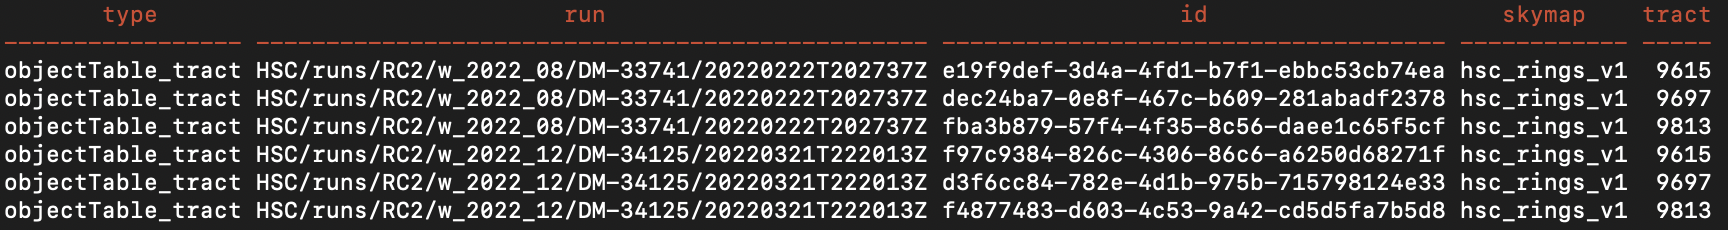
\includegraphics[width=7.91667in]{jira_imgs/2313.png}type
run id skymap tract-----------------
------------------------------------------------
------------------------------------ ------------ -----\\
objectTable\_tract HSC/runs/RC2/w\_2022\_08/DM-33741/20220222T202737Z
e19f9def-3d4a-4fd1-b7f1-ebbc53cb74ea hsc\_rings\_v1~~9615\\
objectTable\_tract HSC/runs/RC2/w\_2022\_08/DM-33741/20220222T202737Z
dec24ba7-0e8f-467c-b609-281abadf2378 hsc\_rings\_v1~~9697\\
objectTable\_tract HSC/runs/RC2/w\_2022\_08/DM-33741/20220222T202737Z
fba3b879-57f4-4f35-8c56-daee1c65f5cf hsc\_rings\_v1~~9813\\
objectTable\_tract HSC/runs/RC2/w\_2022\_12/DM-34125/20220321T222013Z
f97c9384-826c-4306-86c6-a6250d68271f hsc\_rings\_v1~~9615\\
objectTable\_tract HSC/runs/RC2/w\_2022\_12/DM-34125/20220321T222013Z
d3f6cc84-782e-4d1b-975b-715798124e33 hsc\_rings\_v1~~9697\\
objectTable\_tract HSC/runs/RC2/w\_2022\_12/DM-34125/20220321T222013Z
f4877483-d603-4c53-9a42-cd5d5fa7b5d8 hsc\_rings\_v1
9813\\[2\baselineskip]We have thus demonstrated that datasets from
multiple collections can be retrieved by the butler as a single coherent
unit.\\[2\baselineskip]

}

\paragraph{ LVV-T2466 - Verify enable complete pipeline specification }\mbox{}\\

Version \textbf{1}.
Open  \href{https://jira.lsstcorp.org/secure/Tests.jspa#/testCase/LVV-T2466}{\textit{ LVV-T2466 } }
test case in Jira.

Verify that the design provides an interface for delivering a complete
algorithmic work specification (a ``Pipeline specification'') from
Science Pipelines to an execution system, the ``supervisory framework'',
a notable instance of which is the LSST production system.

\textbf{ Preconditions}:\\


Execution status: {\bf Not Executed }

Final comment:\\


Detailed steps results:

\begin{tabular}{p{2cm}p{14cm}}
\toprule
Step 1 & Step Execution Status: \textbf{ Not Executed } \\ \hline
\end{tabular}
 Description \\
{\footnotesize
This is a fundamental part of the design of PipelineTask.

}
\hdashrule[0.5ex]{\textwidth}{1pt}{3mm}
  Expected Result \\
{\footnotesize

}
\hdashrule[0.5ex]{\textwidth}{1pt}{3mm}
  Actual Result \\
{\footnotesize

}

\paragraph{ LVV-T2467 - Verify DataUnit lookup: processing driven }\mbox{}\\

Version \textbf{1}.
Open  \href{https://jira.lsstcorp.org/secure/Tests.jspa#/testCase/LVV-T2467}{\textit{ LVV-T2467 } }
test case in Jira.

Verify that all Data Discovery Systems ~make it possible to discover the
DataUnits for all Datasets that could potentially be used to produce a
given DatasetType with known DataUnits.

\textbf{ Preconditions}:\\


Execution status: {\bf Pass }

Final comment:\\We will verify this by demonstrating that all dataset overlapping a
given tract/patch combination (and thus a specific sky region) can be
readily discovered.~


Detailed steps results:

\begin{tabular}{p{2cm}p{14cm}}
\toprule
Step 1 & Step Execution Status: \textbf{ Pass } \\ \hline
\end{tabular}
 Description \\
{\footnotesize
Run `butler query-datasets` against any major repo (e.g. `/repo/main`).

}
\hdashrule[0.5ex]{\textwidth}{1pt}{3mm}
  Expected Result \\
{\footnotesize

}
\hdashrule[0.5ex]{\textwidth}{1pt}{3mm}
  Actual Result \\
{\footnotesize
This query returns a list of all `calexp` datasets overlapping an
arbitrarily chosen tract (known a priori to contain data in the HSC RC2
dataset), patch combination (9615, 43).\\[2\baselineskip]butler
query-datasets /repo/main calexp --where ``tract=9615 AND patch=43 AND
skymap='hsc\_rings\_v1''' --collections
HSC/runs/RC2/w\_2022\_12/DM-34125 \textbar{} less\\[2\baselineskip]The
first few lines of the returned table are captured in this screenshot:\\
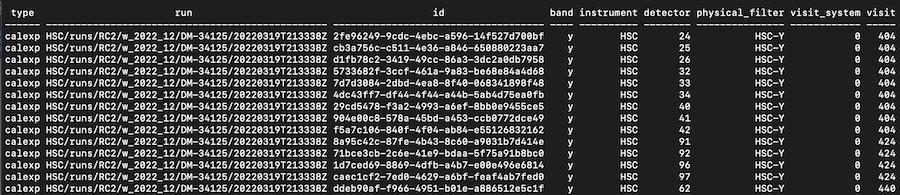
\includegraphics[width=3.12500in]{jira_imgs/2314.png}\\
We have thus demonstrated that dataset discovery by a given set of
DataUnits is enabled by the butler.

}

\paragraph{ LVV-T2464 - Verify multiple simultaneous sky definitions }\mbox{}\\

Version \textbf{1}.
Open  \href{https://jira.lsstcorp.org/secure/Tests.jspa#/testCase/LVV-T2464}{\textit{ LVV-T2464 } }
test case in Jira.

Verify that a collection is able to hold Datasets corresponding to
different sky tilings simultaneously\\[2\baselineskip]

\textbf{ Preconditions}:\\


Execution status: {\bf Pass }

Final comment:\\


Detailed steps results:

\begin{tabular}{p{2cm}p{14cm}}
\toprule
Step 1 & Step Execution Status: \textbf{ Pass } \\ \hline
\end{tabular}
 Description \\
{\footnotesize
Make empty repo.

}
\hdashrule[0.5ex]{\textwidth}{1pt}{3mm}
  Expected Result \\
{\footnotesize

}
\hdashrule[0.5ex]{\textwidth}{1pt}{3mm}
  Actual Result \\
{\footnotesize

}
\begin{tabular}{p{2cm}p{14cm}}
\toprule
Step 2 & Step Execution Status: \textbf{ Pass } \\ \hline
\end{tabular}
 Description \\
{\footnotesize
Run `butler register-skymap`.

}
\hdashrule[0.5ex]{\textwidth}{1pt}{3mm}
  Expected Result \\
{\footnotesize

}
\hdashrule[0.5ex]{\textwidth}{1pt}{3mm}
  Actual Result \\
{\footnotesize

}
\begin{tabular}{p{2cm}p{14cm}}
\toprule
Step 3 & Step Execution Status: \textbf{ Pass } \\ \hline
\end{tabular}
 Description \\
{\footnotesize
Run `butler register-skymap` a second time

}
\hdashrule[0.5ex]{\textwidth}{1pt}{3mm}
  Expected Result \\
{\footnotesize

}
\hdashrule[0.5ex]{\textwidth}{1pt}{3mm}
  Actual Result \\
{\footnotesize
We will start with an existing repository that has more than one
existing skymap. In particular, we will select a repo with recent
reprocessing of the RC2 dataset.

}
\begin{tabular}{p{2cm}p{14cm}}
\toprule
Step 4 & Step Execution Status: \textbf{ Pass } \\ \hline
\end{tabular}
 Description \\
{\footnotesize
Verify that mappings to both tile definitions are valid

}
\hdashrule[0.5ex]{\textwidth}{1pt}{3mm}
  Expected Result \\
{\footnotesize

}
\hdashrule[0.5ex]{\textwidth}{1pt}{3mm}
  Actual Result \\
{\footnotesize
On lsst-devl at NCSA, with the science pipelines set up, opened python
and typed the following:\\[2\baselineskip]import lsst.daf.butler as
dafButler\\
repo =~``/repo/main''\\
butler = dafButler.Butler(repo,
collections={[}``HSC/runs/RC2/w\_2022\_12/DM-34125''{]})\\
registry = butler.registry\\
for d~in registry.queryDimensionRecords(``skymap''):\\
\hspace*{0.333em} ~ print(d)\\[2\baselineskip]This results in the
following screen output:\\[2\baselineskip]skymap:\\
\hspace*{0.333em}\hspace*{0.333em}name: `hsc\_rings\_v1'\\
\hspace*{0.333em}\hspace*{0.333em}hash:
b'\textbackslash{}xe2\textbackslash{}x9f\textbackslash{}xe9\textbackslash{}xf1\textbackslash{}x00\textbackslash{}x8e5\textbackslash{}x9f6\textbackslash{}xa3g\textasciitilde{}\}i\textbackslash{}xccC\textbackslash{}x93v\textbackslash{}xd1\textbackslash{}xe6'\\
\hspace*{0.333em}\hspace*{0.333em}tract\_max: 18938\\
\hspace*{0.333em}\hspace*{0.333em}patch\_nx\_max: 9\\
\hspace*{0.333em}\hspace*{0.333em}patch\_ny\_max: 9\\
skymap:\\
\hspace*{0.333em}\hspace*{0.333em}name: `hsc\_rings\_cells\_v1'\\
\hspace*{0.333em}\hspace*{0.333em}hash:
b'\textbackslash{}xde\textbackslash{}x85\textbackslash{}x13\textbackslash{}xb0q\textbackslash{}x11\textbackslash{}x1e\textbackslash{}x81a\textbackslash{}x9e\textbackslash{}\textbackslash{}\textbackslash{}x06\textbackslash{}x1f\textbackslash{}x02mA\textbackslash{}xf7h\textbackslash{}xe6\textbackslash{}xd4'\\
\hspace*{0.333em}\hspace*{0.333em}tract\_max: 18938\\
\hspace*{0.333em}\hspace*{0.333em}patch\_nx\_max: 11\\
\hspace*{0.333em} patch\_ny\_max: 11\\[2\baselineskip]This demonstrates
that this single collection (``HSC/runs/RC2/w\_2022\_12/DM-34125'')
contains two sky maps with different numbers of patches (i.e., with
different values of patch\_nx\_max and patch\_ny\_max).

}

\paragraph{ LVV-T2465 - Verify pipeline execution in multiple contexts }\mbox{}\\

Version \textbf{1}.
Open  \href{https://jira.lsstcorp.org/secure/Tests.jspa#/testCase/LVV-T2465}{\textit{ LVV-T2465 } }
test case in Jira.

Verify that the design allows a given Pipeline specification to be used
in both development and production contexts.

\textbf{ Preconditions}:\\


Execution status: {\bf Not Executed }

Final comment:\\


Detailed steps results:

\begin{tabular}{p{2cm}p{14cm}}
\toprule
Step 1 & Step Execution Status: \textbf{ Not Executed } \\ \hline
\end{tabular}
 Description \\
{\footnotesize
This is a fundamental part of the design of PipelineTask.

}
\hdashrule[0.5ex]{\textwidth}{1pt}{3mm}
  Expected Result \\
{\footnotesize

}
\hdashrule[0.5ex]{\textwidth}{1pt}{3mm}
  Actual Result \\
{\footnotesize

}

\paragraph{ LVV-T2461 - Verify Collection Layering: Science Platform }\mbox{}\\

Version \textbf{1}.
Open  \href{https://jira.lsstcorp.org/secure/Tests.jspa#/testCase/LVV-T2461}{\textit{ LVV-T2461 } }
test case in Jira.

Verify that collections ~created in the Science Platform are usable as
inputs for processing initiated in the Science Platform

\textbf{ Preconditions}:\\


Execution status: {\bf Not Executed }

Final comment:\\


Detailed steps results:

\begin{tabular}{p{2cm}p{14cm}}
\toprule
Step 1 & Step Execution Status: \textbf{ Not Executed } \\ \hline
\end{tabular}
 Description \\
{\footnotesize
Run part of DRP pipeline in RSP.

}
\hdashrule[0.5ex]{\textwidth}{1pt}{3mm}
  Expected Result \\
{\footnotesize

}
\hdashrule[0.5ex]{\textwidth}{1pt}{3mm}
  Actual Result \\
{\footnotesize

}
\begin{tabular}{p{2cm}p{14cm}}
\toprule
Step 2 & Step Execution Status: \textbf{ Not Executed } \\ \hline
\end{tabular}
 Description \\
{\footnotesize
Run a later part of DRP pipeline in RSP

}
\hdashrule[0.5ex]{\textwidth}{1pt}{3mm}
  Expected Result \\
{\footnotesize

}
\hdashrule[0.5ex]{\textwidth}{1pt}{3mm}
  Actual Result \\
{\footnotesize

}

\paragraph{ LVV-T2463 - Verify enabling of different execution environments }\mbox{}\\

Version \textbf{1}.
Open  \href{https://jira.lsstcorp.org/secure/Tests.jspa#/testCase/LVV-T2463}{\textit{ LVV-T2463 } }
test case in Jira.

Verify that the supervisory framework supports the creation of multiple
specializations for different execution environments.

\textbf{ Preconditions}:\\


Execution status: {\bf Not Executed }

Final comment:\\


Detailed steps results:

\begin{tabular}{p{2cm}p{14cm}}
\toprule
Step 1 & Step Execution Status: \textbf{ Not Executed } \\ \hline
\end{tabular}
 Description \\
{\footnotesize
Satisfied by BPS plugin system; we have plugins for many workflow
systems already.

}
\hdashrule[0.5ex]{\textwidth}{1pt}{3mm}
  Expected Result \\
{\footnotesize

}
\hdashrule[0.5ex]{\textwidth}{1pt}{3mm}
  Actual Result \\
{\footnotesize

}

\paragraph{ LVV-T2462 - Verify QuantumGraph algorithm }\mbox{}\\

Version \textbf{1}.
Open  \href{https://jira.lsstcorp.org/secure/Tests.jspa#/testCase/LVV-T2462}{\textit{ LVV-T2462 } }
test case in Jira.

Verify QuantumGraph algorithm common to all execution environments.
Verify that the supervisory framework provides a common implementation
of the logic required for interpretation of the Pipeline steps and their
data groupings (and thus the possible parallelization); i.e., that the
QuantumGraph generation algorithm can be common to all execution
environments.

\textbf{ Preconditions}:\\


Execution status: {\bf Pass }

Final comment:\\Working on lsst-devl machines in a cloned `pipe\_base` repository at
/project/jcarlin/SVV/gen3\_middleware\_acceptance\_testing/pipe\_base


Detailed steps results:

\begin{tabular}{p{2cm}p{14cm}}
\toprule
Step 1 & Step Execution Status: \textbf{ Pass } \\ \hline
\end{tabular}
 Description \\
{\footnotesize
Execute the test\_graphBuilder.py and test\_quantumGraph.py unit tests
in the \href{https://github.com/lsst/pipe_base/}{pipe\_base}~package.

}
\hdashrule[0.5ex]{\textwidth}{1pt}{3mm}
  Expected Result \\
{\footnotesize
Successful execution of the unit tests.

}
\hdashrule[0.5ex]{\textwidth}{1pt}{3mm}
  Actual Result \\
{\footnotesize
First execute the unit test of a simple graph
builder:\\[2\baselineskip]pytest -s -vv --no-header --cache-clear
tests/test\_graphBuilder.py\\[2\baselineskip]Result:\\[2\baselineskip]tests/test\_graphBuilder.py::FLAKE8~PASSED\\
tests/test\_graphBuilder.py::GraphBuilderTestCase::testAddInstrumentMismatch~PASSED\\
tests/test\_graphBuilder.py::GraphBuilderTestCase::testDefault
PASSED\\[2\baselineskip]Now execute the unit test that more thoroughly
tests quantum graph generation and usage:\\
pytest -s -vv --no-header --cache-clear tests/test\_quantumGraph.py
\textbar{} tee
test\_QG\_log.txt\\[2\baselineskip]tests/test\_quantumGraph.py::FLAKE8
PASSED\\
tests/test\_quantumGraph.py::QuantumGraphTestCase::testAllDatasetTypes
PASSED\\
tests/test\_quantumGraph.py::QuantumGraphTestCase::testContains PASSED\\
tests/test\_quantumGraph.py::QuantumGraphTestCase::testDetermineAnsestorsOfQuantumNode
PASSED\\
tests/test\_quantumGraph.py::QuantumGraphTestCase::testDetermineConnectionsOfQuantum
PASSED\\
tests/test\_quantumGraph.py::QuantumGraphTestCase::testDetermineOutputsOfQuantumNode
PASSED\\
tests/test\_quantumGraph.py::QuantumGraphTestCase::testFindCycle
PASSED\\
tests/test\_quantumGraph.py::QuantumGraphTestCase::testFindQuantaWIthDSType
PASSED\\
tests/test\_quantumGraph.py::QuantumGraphTestCase::testFindTaskDefByLabel
PASSED\\
tests/test\_quantumGraph.py::QuantumGraphTestCase::testFindTaskDefByName
PASSED\\
tests/test\_quantumGraph.py::QuantumGraphTestCase::testFindTasksWithInput
PASSED\\
tests/test\_quantumGraph.py::QuantumGraphTestCase::testFindTasksWithOutput
PASSED\\
tests/test\_quantumGraph.py::QuantumGraphTestCase::testGetNodesForTask
PASSED\\
tests/test\_quantumGraph.py::QuantumGraphTestCase::testGetQuantaForTask
PASSED\\
tests/test\_quantumGraph.py::QuantumGraphTestCase::testGetQuantumNodeByNodeId
PASSED\\
tests/test\_quantumGraph.py::QuantumGraphTestCase::testGraph PASSED\\
tests/test\_quantumGraph.py::QuantumGraphTestCase::testInputQuanta
PASSED\\
tests/test\_quantumGraph.py::QuantumGraphTestCase::testLength PASSED\\
tests/test\_quantumGraph.py::QuantumGraphTestCase::testOutputtQuanta
PASSED\\
tests/test\_quantumGraph.py::QuantumGraphTestCase::testPickle PASSED\\
tests/test\_quantumGraph.py::QuantumGraphTestCase::testSaveLoad PASSED\\
tests/test\_quantumGraph.py::QuantumGraphTestCase::testSaveLoadUri
PASSED\\
tests/test\_quantumGraph.py::QuantumGraphTestCase::testSaveLoadUriS3
PASSED\\
tests/test\_quantumGraph.py::QuantumGraphTestCase::testSubset PASSED\\
tests/test\_quantumGraph.py::QuantumGraphTestCase::testSubsetToConnected
PASSED\\
tests/test\_quantumGraph.py::QuantumGraphTestCase::testTaskGraph
PASSED\\
tests/test\_quantumGraph.py::QuantumGraphTestCase::testTaskWithDSType
PASSED\\
tests/test\_quantumGraph.py::MyMemoryTestCase::testFileDescriptorLeaks
\textless{}-
../../../../../software/lsstsw/stack\_20220215/stack/miniconda3-py38\_4.9.2-2.0.0/Linux64/utils/g617c0b0dc2+9633a190c8/python/lsst/utils/tests.py
PASSED\\[2\baselineskip]All passed. This demonstrates that functional
code is in place for generating quantum graphs.\\[2\baselineskip]

}

\paragraph{ LVV-T2460 - Verify generating a DAG }\mbox{}\\

Version \textbf{1}.
Open  \href{https://jira.lsstcorp.org/secure/Tests.jspa#/testCase/LVV-T2460}{\textit{ LVV-T2460 } }
test case in Jira.

Verify that the supervisory framework supports the ``Pre-flight'' phase
of execution of a Pipeline on a specified set of inputs and/or desired
outputs, resulting in a Directed Acyclic Graph (DAG) for the processing,
with the nodes in the DAG being the units of work to be executed.

\textbf{ Preconditions}:\\


Execution status: {\bf Pass }

Final comment:\\Working on lsst-devl machines in a cloned `pipe\_base` repository
at~/project/jcarlin/SVV/gen3\_middleware\_acceptance\_testing/pipe\_base


Detailed steps results:

\begin{tabular}{p{2cm}p{14cm}}
\toprule
Step 1 & Step Execution Status: \textbf{ Pass } \\ \hline
\end{tabular}
 Description \\
{\footnotesize
Satisfied by existence of QuantumGraph generation code.

}
\hdashrule[0.5ex]{\textwidth}{1pt}{3mm}
  Expected Result \\
{\footnotesize

}
\hdashrule[0.5ex]{\textwidth}{1pt}{3mm}
  Actual Result \\
{\footnotesize
First execute the unit test of a simple graph
builder:\\[2\baselineskip]pytest -s -vv --no-header --cache-clear
tests/test\_graphBuilder.py\\[2\baselineskip]Result:\\[2\baselineskip]tests/test\_graphBuilder.py::FLAKE8~PASSED\\
tests/test\_graphBuilder.py::GraphBuilderTestCase::testAddInstrumentMismatch~PASSED\\
tests/test\_graphBuilder.py::GraphBuilderTestCase::testDefault
PASSED\\[2\baselineskip]Now execute the unit test that more thoroughly
tests quantum graph generation and usage:\\
pytest -s -vv --no-header --cache-clear tests/test\_quantumGraph.py
\textbar{} tee
test\_QG\_log.txt\\[2\baselineskip]tests/test\_quantumGraph.py::FLAKE8
PASSED\\
tests/test\_quantumGraph.py::QuantumGraphTestCase::testAllDatasetTypes
PASSED\\
tests/test\_quantumGraph.py::QuantumGraphTestCase::testContains PASSED\\
tests/test\_quantumGraph.py::QuantumGraphTestCase::testDetermineAnsestorsOfQuantumNode
PASSED\\
tests/test\_quantumGraph.py::QuantumGraphTestCase::testDetermineConnectionsOfQuantum
PASSED\\
tests/test\_quantumGraph.py::QuantumGraphTestCase::testDetermineOutputsOfQuantumNode
PASSED\\
tests/test\_quantumGraph.py::QuantumGraphTestCase::testFindCycle
PASSED\\
tests/test\_quantumGraph.py::QuantumGraphTestCase::testFindQuantaWIthDSType
PASSED\\
tests/test\_quantumGraph.py::QuantumGraphTestCase::testFindTaskDefByLabel
PASSED\\
tests/test\_quantumGraph.py::QuantumGraphTestCase::testFindTaskDefByName
PASSED\\
tests/test\_quantumGraph.py::QuantumGraphTestCase::testFindTasksWithInput
PASSED\\
tests/test\_quantumGraph.py::QuantumGraphTestCase::testFindTasksWithOutput
PASSED\\
tests/test\_quantumGraph.py::QuantumGraphTestCase::testGetNodesForTask
PASSED\\
tests/test\_quantumGraph.py::QuantumGraphTestCase::testGetQuantaForTask
PASSED\\
tests/test\_quantumGraph.py::QuantumGraphTestCase::testGetQuantumNodeByNodeId
PASSED\\
tests/test\_quantumGraph.py::QuantumGraphTestCase::testGraph PASSED\\
tests/test\_quantumGraph.py::QuantumGraphTestCase::testInputQuanta
PASSED\\
tests/test\_quantumGraph.py::QuantumGraphTestCase::testLength PASSED\\
tests/test\_quantumGraph.py::QuantumGraphTestCase::testOutputtQuanta
PASSED\\
tests/test\_quantumGraph.py::QuantumGraphTestCase::testPickle PASSED\\
tests/test\_quantumGraph.py::QuantumGraphTestCase::testSaveLoad PASSED\\
tests/test\_quantumGraph.py::QuantumGraphTestCase::testSaveLoadUri
PASSED\\
tests/test\_quantumGraph.py::QuantumGraphTestCase::testSaveLoadUriS3
PASSED\\
tests/test\_quantumGraph.py::QuantumGraphTestCase::testSubset PASSED\\
tests/test\_quantumGraph.py::QuantumGraphTestCase::testSubsetToConnected
PASSED\\
tests/test\_quantumGraph.py::QuantumGraphTestCase::testTaskGraph
PASSED\\
tests/test\_quantumGraph.py::QuantumGraphTestCase::testTaskWithDSType
PASSED\\
tests/test\_quantumGraph.py::MyMemoryTestCase::testFileDescriptorLeaks
\textless{}-
../../../../../software/lsstsw/stack\_20220215/stack/miniconda3-py38\_4.9.2-2.0.0/Linux64/utils/g617c0b0dc2+9633a190c8/python/lsst/utils/tests.py
PASSED\\[2\baselineskip]All passed. This demonstrates that functional
code is in place for DAG generation.\\[2\baselineskip]

}

\paragraph{ LVV-T2457 - Verify butler instantiation }\mbox{}\\

Version \textbf{1}.
Open  \href{https://jira.lsstcorp.org/secure/Tests.jspa#/testCase/LVV-T2457}{\textit{ LVV-T2457 } }
test case in Jira.

Verify that the supervisory framework creates and supplies the Butler
required to support the I/O to be performed in the ``Run'' phase, for
each unit of work.

\textbf{ Preconditions}:\\


Execution status: {\bf Not Executed }

Final comment:\\


Detailed steps results:

\begin{tabular}{p{2cm}p{14cm}}
\toprule
Step 1 & Step Execution Status: \textbf{ Not Executed } \\ \hline
\end{tabular}
 Description \\
{\footnotesize

}
\hdashrule[0.5ex]{\textwidth}{1pt}{3mm}
  Expected Result \\
{\footnotesize

}
\hdashrule[0.5ex]{\textwidth}{1pt}{3mm}
  Actual Result \\
{\footnotesize

}

\paragraph{ LVV-T2456 - Verify execution logging }\mbox{}\\

Version \textbf{1}.
Open  \href{https://jira.lsstcorp.org/secure/Tests.jspa#/testCase/LVV-T2456}{\textit{ LVV-T2456 } }
test case in Jira.

Verify that standard logging is enabled for the pre-flight and run
processes of pipelines.

\textbf{ Preconditions}:\\


Execution status: {\bf Not Executed }

Final comment:\\


Detailed steps results:

\begin{tabular}{p{2cm}p{14cm}}
\toprule
Step 1 & Step Execution Status: \textbf{ Not Executed } \\ \hline
\end{tabular}
 Description \\
{\footnotesize

}
\hdashrule[0.5ex]{\textwidth}{1pt}{3mm}
  Expected Result \\
{\footnotesize

}
\hdashrule[0.5ex]{\textwidth}{1pt}{3mm}
  Actual Result \\
{\footnotesize

}

\paragraph{ LVV-T2455 - Verify pipeline interface available as Python API }\mbox{}\\

Version \textbf{1}.
Open  \href{https://jira.lsstcorp.org/secure/Tests.jspa#/testCase/LVV-T2455}{\textit{ LVV-T2455 } }
test case in Jira.

Verify that the Pipeline specification interface is available as a
Python API.

\textbf{ Preconditions}:\\


Execution status: {\bf Not Executed }

Final comment:\\


Detailed steps results:

\begin{tabular}{p{2cm}p{14cm}}
\toprule
Step 1 & Step Execution Status: \textbf{ Not Executed } \\ \hline
\end{tabular}
 Description \\
{\footnotesize

}
\hdashrule[0.5ex]{\textwidth}{1pt}{3mm}
  Expected Result \\
{\footnotesize

}
\hdashrule[0.5ex]{\textwidth}{1pt}{3mm}
  Actual Result \\
{\footnotesize

}

\paragraph{ LVV-T2454 - Verify pre-execution config overrides }\mbox{}\\

Version \textbf{1}.
Open  \href{https://jira.lsstcorp.org/secure/Tests.jspa#/testCase/LVV-T2454}{\textit{ LVV-T2454 } }
test case in Jira.

Verify that the middleware enables programmatic overrides to the
configurations specified for a Pipeline, and that the overrides can be
captured for purposes of provenance recording.

\textbf{ Preconditions}:\\


Execution status: {\bf Not Executed }

Final comment:\\


Detailed steps results:

\begin{tabular}{p{2cm}p{14cm}}
\toprule
Step 1 & Step Execution Status: \textbf{ Not Executed } \\ \hline
\end{tabular}
 Description \\
{\footnotesize

}
\hdashrule[0.5ex]{\textwidth}{1pt}{3mm}
  Expected Result \\
{\footnotesize

}
\hdashrule[0.5ex]{\textwidth}{1pt}{3mm}
  Actual Result \\
{\footnotesize

}

\paragraph{ LVV-T2458 - Verify serialization of pre-flight results }\mbox{}\\

Version \textbf{1}.
Open  \href{https://jira.lsstcorp.org/secure/Tests.jspa#/testCase/LVV-T2458}{\textit{ LVV-T2458 } }
test case in Jira.

Verify that the supervisory framework provides a serialization form for
the results of the ``Pre-flight'' phase, so that they can be computed in
one process and executed under the control of one or more others.

\textbf{ Preconditions}:\\


Execution status: {\bf Not Executed }

Final comment:\\


Detailed steps results:

\begin{tabular}{p{2cm}p{14cm}}
\toprule
Step 1 & Step Execution Status: \textbf{ Not Executed } \\ \hline
\end{tabular}
 Description \\
{\footnotesize
Satisfied by QuantumGraph being serializable.

}
\hdashrule[0.5ex]{\textwidth}{1pt}{3mm}
  Expected Result \\
{\footnotesize

}
\hdashrule[0.5ex]{\textwidth}{1pt}{3mm}
  Actual Result \\
{\footnotesize

}

\paragraph{ LVV-T2451 - Verify ability to append to an existing repository }\mbox{}\\

Version \textbf{1}.
Open  \href{https://jira.lsstcorp.org/secure/Tests.jspa#/testCase/LVV-T2451}{\textit{ LVV-T2451 } }
test case in Jira.

Verify that it is possible to add Datasets to a pre-existing Collection
via additional processing.

\textbf{ Preconditions}:\\


Execution status: {\bf Not Executed }

Final comment:\\


Detailed steps results:

\begin{tabular}{p{2cm}p{14cm}}
\toprule
Step 1 & Step Execution Status: \textbf{ Not Executed } \\ \hline
\end{tabular}
 Description \\
{\footnotesize
In regular use in production and included in unit tests. -- WHICH UNIT
TESTS?

}
\hdashrule[0.5ex]{\textwidth}{1pt}{3mm}
  Expected Result \\
{\footnotesize
Unit test passes

}
\hdashrule[0.5ex]{\textwidth}{1pt}{3mm}
  Actual Result \\
{\footnotesize

}

\paragraph{ LVV-T2453 - Verify creation of DatasetRef upon butler.put }\mbox{}\\

Version \textbf{1}.
Open  \href{https://jira.lsstcorp.org/secure/Tests.jspa#/testCase/LVV-T2453}{\textit{ LVV-T2453 } }
test case in Jira.

Verify that upon writing a dataset, a DatasetRef is created to enable
getting the dataset in the future.

\textbf{ Preconditions}:\\


Execution status: {\bf Pass }

Final comment:\\


Detailed steps results:

\begin{tabular}{p{2cm}p{14cm}}
\toprule
Step 1 & Step Execution Status: \textbf{ Pass } \\ \hline
\end{tabular}
 Description \\
{\footnotesize
Execute ButlerPutGetTests
in~\url{https://github.com/lsst/daf_butler/blob/main/tests/test_butler.py}

}
\hdashrule[0.5ex]{\textwidth}{1pt}{3mm}
  Expected Result \\
{\footnotesize
Unit test passes

}
\hdashrule[0.5ex]{\textwidth}{1pt}{3mm}
  Actual Result \\
{\footnotesize
On lsst-devl machines at NCSA, in a cloned `daf\_butler` repository (at
/project/jcarlin/SVV/gen3\_middleware\_acceptance\_testing/daf\_butler),
execute:\\[2\baselineskip]pytest -s -vv --no-header --cache-clear
tests/test\_butler.py\\[2\baselineskip]Results:\\
tests/test\_butler.py::PosixDatastoreButlerTestCase::testBasicPutGet~PASSED\\
tests/test\_butler.py::PosixDatastoreButlerTestCase::testButlerRewriteDataId
PASSED\\
tests/test\_butler.py::PosixDatastoreButlerTestCase::testCompositePutGetConcrete
PASSED\\
tests/test\_butler.py::PosixDatastoreButlerTestCase::testCompositePutGetVirtual
PASSED\\
tests/test\_butler.py::InMemoryDatastoreButlerTestCase::testBasicPutGet~PASSED\\
tests/test\_butler.py::InMemoryDatastoreButlerTestCase::testButlerRewriteDataId
PASSED\\
tests/test\_butler.py::InMemoryDatastoreButlerTestCase::testCompositePutGetConcrete
PASSED\\
tests/test\_butler.py::InMemoryDatastoreButlerTestCase::testCompositePutGetVirtual
PASSED\\
tests/test\_butler.py::ChainedDatastoreButlerTestCase::testBasicPutGet~PASSED\\
tests/test\_butler.py::ChainedDatastoreButlerTestCase::testButlerRewriteDataId
PASSED\\
tests/test\_butler.py::ChainedDatastoreButlerTestCase::testCompositePutGetConcrete
PASSED\\
tests/test\_butler.py::ChainedDatastoreButlerTestCase::testCompositePutGetVirtual
PASSED\\
tests/test\_butler.py::ButlerExplicitRootTestCase::testBasicPutGet~PASSED\\
tests/test\_butler.py::ButlerExplicitRootTestCase::testButlerRewriteDataId
PASSED\\
tests/test\_butler.py::ButlerExplicitRootTestCase::testCompositePutGetConcrete
PASSED\\
tests/test\_butler.py::ButlerExplicitRootTestCase::testCompositePutGetVirtual
PASSED\\
tests/test\_butler.py::ButlerMakeRepoOutfileTestCase::testPutGet~PASSED\\
tests/test\_butler.py::ButlerMakeRepoOutfileDirTestCase::testConfigExistence
PASSED\\
tests/test\_butler.py::ButlerMakeRepoOutfileDirTestCase::testDeferredCollectionPassing
PASSED\\
tests/test\_butler.py::ButlerMakeRepoOutfileDirTestCase::testPutGet~PASSED\\
tests/test\_butler.py::ButlerMakeRepoOutfileUriTestCase::testConfigExistence
PASSED\\
tests/test\_butler.py::ButlerMakeRepoOutfileUriTestCase::testDeferredCollectionPassing
PASSED\\
tests/test\_butler.py::ButlerMakeRepoOutfileUriTestCase::testPutGet~PASSED\\
tests/test\_butler.py::S3DatastoreButlerTestCase::testBasicPutGet~PASSED\\
tests/test\_butler.py::S3DatastoreButlerTestCase::testButlerRewriteDataId
PASSED\\
tests/test\_butler.py::S3DatastoreButlerTestCase::testCompositePutGetConcrete
PASSED\\
tests/test\_butler.py::S3DatastoreButlerTestCase::testCompositePutGetVirtual
PASSED\\[2\baselineskip]All tests of the butler's ``Put'' and ``Get''
functionality passed.

}

\paragraph{ LVV-T2449 - Verify middleware writer configurability }\mbox{}\\

Version \textbf{1}.
Open  \href{https://jira.lsstcorp.org/secure/Tests.jspa#/testCase/LVV-T2449}{\textit{ LVV-T2449 } }
test case in Jira.

Verify that the data output system supports configuration of individual
writer behavior.

\textbf{ Preconditions}:\\


Execution status: {\bf Pass }

Final comment:\\


Detailed steps results:

\begin{tabular}{p{2cm}p{14cm}}
\toprule
Step 1 & Step Execution Status: \textbf{ Pass } \\ \hline
\end{tabular}
 Description \\
{\footnotesize
Execute the unit test at
\url{https://github.com/lsst/daf_butler/blob/main/tests/test_config.py},
which tests the writer configuration.

}
\hdashrule[0.5ex]{\textwidth}{1pt}{3mm}
  Expected Result \\
{\footnotesize
Unit test passes.

}
\hdashrule[0.5ex]{\textwidth}{1pt}{3mm}
  Actual Result \\
{\footnotesize
On lsst-devl machines at NCSA, in a cloned `daf\_butler` repository (at
/project/jcarlin/SVV/gen3\_middleware\_acceptance\_testing/daf\_butler),
execute:\\[2\baselineskip]pytest -s -vv --no-header --cache-clear
tests/test\_config.py\\[2\baselineskip]Results:\\[2\baselineskip]tests/test\_config.py::FLAKE8
PASSED\\
tests/test\_config.py::ConfigTestCase::testBadConfig~PASSED\\
tests/test\_config.py::ConfigTestCase::testBasics~PASSED\\
tests/test\_config.py::ConfigTestCase::testDict~PASSED\\
tests/test\_config.py::ConfigTestCase::testEscape~PASSED\\
tests/test\_config.py::ConfigTestCase::testHierarchy~PASSED\\
tests/test\_config.py::ConfigTestCase::testMerge~PASSED\\
tests/test\_config.py::ConfigTestCase::testOperators~PASSED\\
tests/test\_config.py::ConfigTestCase::testSerializedString~PASSED\\
tests/test\_config.py::ConfigTestCase::testSplitting~PASSED\\
tests/test\_config.py::ConfigTestCase::testUpdate~PASSED\\
tests/test\_config.py::ConfigSubsetTestCase::testAbsPath~PASSED\\
tests/test\_config.py::ConfigSubsetTestCase::testClassDerived~PASSED\\
tests/test\_config.py::ConfigSubsetTestCase::testDefaults~PASSED\\
tests/test\_config.py::ConfigSubsetTestCase::testEmpty~PASSED\\
tests/test\_config.py::ConfigSubsetTestCase::testExternalHierarchy~PASSED\\
tests/test\_config.py::ConfigSubsetTestCase::testExternalOverride~PASSED\\
tests/test\_config.py::ConfigSubsetTestCase::testInclude~PASSED\\
tests/test\_config.py::ConfigSubsetTestCase::testIncludeConfigs~PASSED\\
tests/test\_config.py::ConfigSubsetTestCase::testNoDefaults~PASSED\\
tests/test\_config.py::ConfigSubsetTestCase::testPathlib~PASSED\\
tests/test\_config.py::ConfigSubsetTestCase::testResource~PASSED\\
tests/test\_config.py::ConfigSubsetTestCase::testSearchPaths~PASSED\\
tests/test\_config.py::ConfigSubsetTestCase::testStringInclude~PASSED\\
tests/test\_config.py::FileWriteConfigTestCase::testDump
PASSED\\[2\baselineskip]This confirms that the writer behavior can be
configured.

}

\paragraph{ LVV-T2452 - Verify specification of output locations }\mbox{}\\

Version \textbf{1}.
Open  \href{https://jira.lsstcorp.org/secure/Tests.jspa#/testCase/LVV-T2452}{\textit{ LVV-T2452 } }
test case in Jira.

Verify that the middleware enables configuration of the output location
for a POSIX file system.

\textbf{ Preconditions}:\\


Execution status: {\bf Pass }

Final comment:\\Working with a cloned `daf\_butler` repository
at~/project/jcarlin/SVV/gen3\_middleware\_acceptance\_testing/daf\_butler
on the lsst-devl machines.


Detailed steps results:

\begin{tabular}{p{2cm}p{14cm}}
\toprule
Step 1 & Step Execution Status: \textbf{ Pass } \\ \hline
\end{tabular}
 Description \\
{\footnotesize
Execute the PosixDatastoreButlerTestCase in
\url{https://github.com/lsst/daf_butler/blob/main/tests/test_butler.py}

}
\hdashrule[0.5ex]{\textwidth}{1pt}{3mm}
  Expected Result \\
{\footnotesize
Unit test passes

}
\hdashrule[0.5ex]{\textwidth}{1pt}{3mm}
  Actual Result \\
{\footnotesize
Executed the unit test via: ``pytest -s -vv --no-header
tests/test\_butler.py''\\[2\baselineskip]Results:\\[2\baselineskip]tests/test\_butler.py::PosixDatastoreButlerTestCase::testBasicPutGet
PASSED\\
tests/test\_butler.py::PosixDatastoreButlerTestCase::testButlerRewriteDataId
PASSED\\
tests/test\_butler.py::PosixDatastoreButlerTestCase::testCompositePutGetConcrete
PASSED\\
tests/test\_butler.py::PosixDatastoreButlerTestCase::testCompositePutGetVirtual
PASSED\\
tests/test\_butler.py::PosixDatastoreButlerTestCase::testConstructor
PASSED\\
tests/test\_butler.py::PosixDatastoreButlerTestCase::testDeferredCollectionPassing
PASSED\\
tests/test\_butler.py::PosixDatastoreButlerTestCase::testExportTransferCopy
PASSED\\
tests/test\_butler.py::PosixDatastoreButlerTestCase::testGetDatasetTypes
PASSED\\
tests/test\_butler.py::PosixDatastoreButlerTestCase::testImportExport
Root:
file:///project/jcarlin/SVV/gen3\_middleware\_acceptance\_testing/daf\_butler/tests/tmpdke1g8no/\\
PASSED\\
tests/test\_butler.py::PosixDatastoreButlerTestCase::testImportExportVirtualComposite
Root:
file:///project/jcarlin/SVV/gen3\_middleware\_acceptance\_testing/daf\_butler/tests/tmpdd9i5by4/\\
XFAIL\\
tests/test\_butler.py::PosixDatastoreButlerTestCase::testIngest PASSED\\
tests/test\_butler.py::PosixDatastoreButlerTestCase::testMakeRepo
PASSED\\
tests/test\_butler.py::PosixDatastoreButlerTestCase::testPathConstructor
PASSED\\
tests/test\_butler.py::PosixDatastoreButlerTestCase::testPickle PASSED\\
tests/test\_butler.py::PosixDatastoreButlerTestCase::testPruneCollections
PASSED\\
tests/test\_butler.py::PosixDatastoreButlerTestCase::testPruneDatasets
PASSED\\
tests/test\_butler.py::PosixDatastoreButlerTestCase::testPutTemplates
PASSED\\
tests/test\_butler.py::PosixDatastoreButlerTestCase::testPytypeCoercion
PASSED\\
tests/test\_butler.py::PosixDatastoreButlerTestCase::testPytypePutCoercion
PASSED\\
tests/test\_butler.py::PosixDatastoreButlerTestCase::testRemoveRuns
PASSED\\
tests/test\_butler.py::PosixDatastoreButlerTestCase::testStringification
PASSED\\
tests/test\_butler.py::PosixDatastoreButlerTestCase::testTransaction
PASSED\\[2\baselineskip]All of the tests in PosixDatastoreButlerTestCase
have passed.

}

\paragraph{ LVV-T2450 - Verify writing dataset to multiple repositories }\mbox{}\\

Version \textbf{1}.
Open  \href{https://jira.lsstcorp.org/secure/Tests.jspa#/testCase/LVV-T2450}{\textit{ LVV-T2450 } }
test case in Jira.

Verify that the middleware enables writing of a single dataset to
multiple repositories, with a different output format used for each
repository.

\textbf{ Preconditions}:\\


Execution status: {\bf Not Executed }

Final comment:\\


Detailed steps results:

\begin{tabular}{p{2cm}p{14cm}}
\toprule
Step 1 & Step Execution Status: \textbf{ Not Executed } \\ \hline
\end{tabular}
 Description \\
{\footnotesize
Not regularly exercised in production, but functionality is tested in
daf\_butler unit tests. --- WHICH UNIT TESTS?

}
\hdashrule[0.5ex]{\textwidth}{1pt}{3mm}
  Expected Result \\
{\footnotesize
Unit test passes

}
\hdashrule[0.5ex]{\textwidth}{1pt}{3mm}
  Actual Result \\
{\footnotesize

}

\paragraph{ LVV-T2447 - Verify DataRepository layering: Data Release and Science Platform }\mbox{}\\

Version \textbf{1}.
Open  \href{https://jira.lsstcorp.org/secure/Tests.jspa#/testCase/LVV-T2447}{\textit{ LVV-T2447 } }
test case in Jira.

Verify that a Data Release is usable as the inputs for processing
initiated in the Science Platform.

\textbf{ Preconditions}:\\


Execution status: {\bf Not Executed }

Final comment:\\


Detailed steps results:

\begin{tabular}{p{2cm}p{14cm}}
\toprule
Step 1 & Step Execution Status: \textbf{ Not Executed } \\ \hline
\end{tabular}
 Description \\
{\footnotesize
Reuse test scirpt for DMS-MWBT-REQ-0012

}
\hdashrule[0.5ex]{\textwidth}{1pt}{3mm}
  Expected Result \\
{\footnotesize

}
\hdashrule[0.5ex]{\textwidth}{1pt}{3mm}
  Actual Result \\
{\footnotesize

}
\begin{tabular}{p{2cm}p{14cm}}
\toprule
Step 2 & Step Execution Status: \textbf{ Not Executed } \\ \hline
\end{tabular}
 Description \\
{\footnotesize
Run a DRP pipeline subset in RSP, using DP0.x collections as inputs.

}
\hdashrule[0.5ex]{\textwidth}{1pt}{3mm}
  Expected Result \\
{\footnotesize

}
\hdashrule[0.5ex]{\textwidth}{1pt}{3mm}
  Actual Result \\
{\footnotesize

}

\paragraph{ LVV-T2446 - Verify registries of collections }\mbox{}\\

Version \textbf{1}.
Open  \href{https://jira.lsstcorp.org/secure/Tests.jspa#/testCase/LVV-T2446}{\textit{ LVV-T2446 } }
test case in Jira.

Verify that there is a ~mechanism for registering Collections as they
are created

\textbf{ Preconditions}:\\


Execution status: {\bf Not Executed }

Final comment:\\


Detailed steps results:

\begin{tabular}{p{2cm}p{14cm}}
\toprule
Step 1 & Step Execution Status: \textbf{ Not Executed } \\ \hline
\end{tabular}
 Description \\
{\footnotesize

}
\hdashrule[0.5ex]{\textwidth}{1pt}{3mm}
  Expected Result \\
{\footnotesize

}
\hdashrule[0.5ex]{\textwidth}{1pt}{3mm}
  Actual Result \\
{\footnotesize

}

\paragraph{ LVV-T2444 - Verify dataset garbage collection }\mbox{}\\

Version \textbf{1}.
Open  \href{https://jira.lsstcorp.org/secure/Tests.jspa#/testCase/LVV-T2444}{\textit{ LVV-T2444 } }
test case in Jira.

Verify that when a DataRepository is removed, the Datasets it references
are removed if and only if they are not also referenced by one or more
additional DataRepositories that have been explicitly
identified.\\[2\baselineskip]Note that the requirement text assumed a
slightly different collections model from what we have.~ ~ ~Instead of
``reference counting'' datasets, we have RUN collections that own
datasets and TAGGED collections that don't, but we still guard against
improper deletions as the requirement demands.

\textbf{ Preconditions}:\\


Execution status: {\bf Not Executed }

Final comment:\\


Detailed steps results:

\begin{tabular}{p{2cm}p{14cm}}
\toprule
Step 1 & Step Execution Status: \textbf{ Not Executed } \\ \hline
\end{tabular}
 Description \\
{\footnotesize
Make example repo, one each, ~POSIX and S3

}
\hdashrule[0.5ex]{\textwidth}{1pt}{3mm}
  Expected Result \\
{\footnotesize

}
\hdashrule[0.5ex]{\textwidth}{1pt}{3mm}
  Actual Result \\
{\footnotesize

}
\begin{tabular}{p{2cm}p{14cm}}
\toprule
Step 2 & Step Execution Status: \textbf{ Not Executed } \\ \hline
\end{tabular}
 Description \\
{\footnotesize
Create TAGGED collection and add some datasets to it.

}
\hdashrule[0.5ex]{\textwidth}{1pt}{3mm}
  Expected Result \\
{\footnotesize

}
\hdashrule[0.5ex]{\textwidth}{1pt}{3mm}
  Actual Result \\
{\footnotesize

}
\begin{tabular}{p{2cm}p{14cm}}
\toprule
Step 3 & Step Execution Status: \textbf{ Not Executed } \\ \hline
\end{tabular}
 Description \\
{\footnotesize
Try to delete the RUN collection - shouldn't be possible because of
references in TAGGED collection.

}
\hdashrule[0.5ex]{\textwidth}{1pt}{3mm}
  Expected Result \\
{\footnotesize

}
\hdashrule[0.5ex]{\textwidth}{1pt}{3mm}
  Actual Result \\
{\footnotesize

}
\begin{tabular}{p{2cm}p{14cm}}
\toprule
Step 4 & Step Execution Status: \textbf{ Not Executed } \\ \hline
\end{tabular}
 Description \\
{\footnotesize
Try to delete the TAGGED collection - should work, without deleting the
datasets.

}
\hdashrule[0.5ex]{\textwidth}{1pt}{3mm}
  Expected Result \\
{\footnotesize

}
\hdashrule[0.5ex]{\textwidth}{1pt}{3mm}
  Actual Result \\
{\footnotesize

}

\paragraph{ LVV-T2442 - Verify dataset deletion }\mbox{}\\

Version \textbf{1}.
Open  \href{https://jira.lsstcorp.org/secure/Tests.jspa#/testCase/LVV-T2442}{\textit{ LVV-T2442 } }
test case in Jira.

Verify that a Dataset is deletable from a DataRepository by an
authorized person.

\textbf{ Preconditions}:\\


Execution status: {\bf Initial Pass }

Final comment:\\


Detailed steps results:

\begin{tabular}{p{2cm}p{14cm}}
\toprule
Step 1 & Step Execution Status: \textbf{ Initial Pass } \\ \hline
\end{tabular}
 Description \\
{\footnotesize
Make example repo, one each,~ POSIX and S3

}
\hdashrule[0.5ex]{\textwidth}{1pt}{3mm}
  Expected Result \\
{\footnotesize

}
\hdashrule[0.5ex]{\textwidth}{1pt}{3mm}
  Actual Result \\
{\footnotesize

}
\begin{tabular}{p{2cm}p{14cm}}
\toprule
Step 2 & Step Execution Status: \textbf{ Pass } \\ \hline
\end{tabular}
 Description \\
{\footnotesize
Run `butler prune-datasets`

}
\hdashrule[0.5ex]{\textwidth}{1pt}{3mm}
  Expected Result \\
{\footnotesize

}
\hdashrule[0.5ex]{\textwidth}{1pt}{3mm}
  Actual Result \\
{\footnotesize
On lsst-devl machines at NCSA, in a cloned `daf\_butler` repository (at
/project/jcarlin/SVV/gen3\_middleware\_acceptance\_testing/daf\_butler),
execute:\\[2\baselineskip]pytest -s -vv --no-header --cache-clear
tests/test\_cliCmdPruneDatasets.py\\[2\baselineskip]The results show
that the deletion of datasets was
successful:\\[2\baselineskip]tests/test\_cliCmdPruneDatasets.py::FLAKE8~PASSED\\
tests/test\_cliCmdPruneDatasets.py::PruneDatasetsTestCase::test\_defaults\_doContinue~PASSED\\
tests/test\_cliCmdPruneDatasets.py::PruneDatasetsTestCase::test\_defaults\_doNotContinue~PASSED\\
tests/test\_cliCmdPruneDatasets.py::PruneDatasetsTestCase::test\_disassociateImpliedArgs~PASSED\\
tests/test\_cliCmdPruneDatasets.py::PruneDatasetsTestCase::test\_disassociateImpliedArgsWithCollections~PASSED\\
tests/test\_cliCmdPruneDatasets.py::PruneDatasetsTestCase::test\_dryRun\_disassociate~PASSED\\
tests/test\_cliCmdPruneDatasets.py::PruneDatasetsTestCase::test\_dryRun\_unstore~PASSED\\
tests/test\_cliCmdPruneDatasets.py::PruneDatasetsTestCase::test\_dryRun\_unstoreAndDisassociate~PASSED\\
tests/test\_cliCmdPruneDatasets.py::PruneDatasetsTestCase::test\_noCollections~PASSED\\
tests/test\_cliCmdPruneDatasets.py::PruneDatasetsTestCase::test\_noConfirm~PASSED\\
tests/test\_cliCmdPruneDatasets.py::PruneDatasetsTestCase::test\_noDatasets~PASSED\\
tests/test\_cliCmdPruneDatasets.py::PruneDatasetsTestCase::test\_purgeImpliedArgs~PASSED\\
tests/test\_cliCmdPruneDatasets.py::PruneDatasetsTestCase::test\_purgeImpliedArgsWithCollections~PASSED\\
tests/test\_cliCmdPruneDatasets.py::PruneDatasetsTestCase::test\_purgeOnNonRunCollection~PASSED\\
tests/test\_cliCmdPruneDatasets.py::PruneDatasetsTestCase::test\_purgeWithDisassociate~PASSED\\
tests/test\_cliCmdPruneDatasets.py::PruneDatasetsTestCase::test\_quiet~PASSED\\
tests/test\_cliCmdPruneDatasets.py::PruneDatasetsTestCase::test\_quietWithDryRun~PASSED\\[2\baselineskip]

}
\begin{tabular}{p{2cm}p{14cm}}
\toprule
Step 3 & Step Execution Status: \textbf{ Pass } \\ \hline
\end{tabular}
 Description \\
{\footnotesize
Verify that the datasets are deleted

}
\hdashrule[0.5ex]{\textwidth}{1pt}{3mm}
  Expected Result \\
{\footnotesize

}
\hdashrule[0.5ex]{\textwidth}{1pt}{3mm}
  Actual Result \\
{\footnotesize
The unit test includes steps that confirm the deletion of the datasets.~

}

\paragraph{ LVV-T2443 - Verify repository removal }\mbox{}\\

Version \textbf{1}.
Open  \href{https://jira.lsstcorp.org/secure/Tests.jspa#/testCase/LVV-T2443}{\textit{ LVV-T2443 } }
test case in Jira.

Verify that an authorized user can remove a DataRepository from any
storage environment. Verification on \textbf{all} environments is not
possible. We will verify POSIX and S3 environments, which we believe is
in the spirit of the requirement and covers our core needs.

\textbf{ Preconditions}:\\


Execution status: {\bf Initial Pass }

Final comment:\\


Detailed steps results:

\begin{tabular}{p{2cm}p{14cm}}
\toprule
Step 1 & Step Execution Status: \textbf{ Initial Pass } \\ \hline
\end{tabular}
 Description \\
{\footnotesize
Make example repo, one each, ~POSIX and S3

}
\hdashrule[0.5ex]{\textwidth}{1pt}{3mm}
  Expected Result \\
{\footnotesize

}
\hdashrule[0.5ex]{\textwidth}{1pt}{3mm}
  Actual Result \\
{\footnotesize
Tested on a POSIX datastore at NCSA (lsst-devl machines).

}
\begin{tabular}{p{2cm}p{14cm}}
\toprule
Step 2 & Step Execution Status: \textbf{ Pass } \\ \hline
\end{tabular}
 Description \\
{\footnotesize
Run `butler prune-collection`

}
\hdashrule[0.5ex]{\textwidth}{1pt}{3mm}
  Expected Result \\
{\footnotesize

}
\hdashrule[0.5ex]{\textwidth}{1pt}{3mm}
  Actual Result \\
{\footnotesize
On lsst-devl machines at NCSA, in a cloned `daf\_butler` repository (at
/project/jcarlin/SVV/gen3\_middleware\_acceptance\_testing/daf\_butler),
execute:\\[2\baselineskip]pytest -s -vv --no-header --cache-clear
tests/test\_cliCmdPruneCollection.py\\[2\baselineskip]The results show
that the pruning of collections is
successful:\\[2\baselineskip]tests/test\_cliCmdPruneCollection.py::FLAKE8
PASSED\\
tests/test\_cliCmdPruneCollection.py::PruneCollectionsTest::testPruneCollections~PASSED\\
tests/test\_cliCmdPruneCollection.py::PruneCollectionExecutionTest::testPruneRun~PASSED\\
tests/test\_cliCmdPruneCollection.py::PruneCollectionExecutionTest::testPruneTagged
PASSED

}
\begin{tabular}{p{2cm}p{14cm}}
\toprule
Step 3 & Step Execution Status: \textbf{ Pass } \\ \hline
\end{tabular}
 Description \\
{\footnotesize
Verify that the repository is removed

}
\hdashrule[0.5ex]{\textwidth}{1pt}{3mm}
  Expected Result \\
{\footnotesize

}
\hdashrule[0.5ex]{\textwidth}{1pt}{3mm}
  Actual Result \\
{\footnotesize
The unit test includes checks that the collection has been removed.

}

\paragraph{ LVV-T2441 - Verify repository version migration }\mbox{}\\

Version \textbf{1}.
Open  \href{https://jira.lsstcorp.org/secure/Tests.jspa#/testCase/LVV-T2441}{\textit{ LVV-T2441 } }
test case in Jira.

Verify that the Data Input/Output system can perform persistent
migrations of a DataRepository to bring the Data Model of that
DataRepository up to parity with the Data Model expected by the current
Data Input/Output System interfaces.\\[2\baselineskip]

\textbf{ Preconditions}:\\


Execution status: {\bf Not Executed }

Final comment:\\


Detailed steps results:

\begin{tabular}{p{2cm}p{14cm}}
\toprule
Step 1 & Step Execution Status: \textbf{ Not Executed } \\ \hline
\end{tabular}
 Description \\
{\footnotesize
Make example repo with one schema configuration (e.g. autoincrement
dataset IDs).\\[2\baselineskip]

}
\hdashrule[0.5ex]{\textwidth}{1pt}{3mm}
  Expected Result \\
{\footnotesize

}
\hdashrule[0.5ex]{\textwidth}{1pt}{3mm}
  Actual Result \\
{\footnotesize

}
\begin{tabular}{p{2cm}p{14cm}}
\toprule
Step 2 & Step Execution Status: \textbf{ Not Executed } \\ \hline
\end{tabular}
 Description \\
{\footnotesize
Run existing migration script that upgrades the repository to the new
one.

}
\hdashrule[0.5ex]{\textwidth}{1pt}{3mm}
  Expected Result \\
{\footnotesize

}
\hdashrule[0.5ex]{\textwidth}{1pt}{3mm}
  Actual Result \\
{\footnotesize

}
\begin{tabular}{p{2cm}p{14cm}}
\toprule
Step 3 & Step Execution Status: \textbf{ Not Executed } \\ \hline
\end{tabular}
 Description \\
{\footnotesize
Verify that the features are migrated correctly

}
\hdashrule[0.5ex]{\textwidth}{1pt}{3mm}
  Expected Result \\
{\footnotesize

}
\hdashrule[0.5ex]{\textwidth}{1pt}{3mm}
  Actual Result \\
{\footnotesize

}

\paragraph{ LVV-T2440 - Verify versioning of DataRepositories }\mbox{}\\

Version \textbf{1}.
Open  \href{https://jira.lsstcorp.org/secure/Tests.jspa#/testCase/LVV-T2440}{\textit{ LVV-T2440 } }
test case in Jira.

Verify that the ~Data Input/Output system can describe the version of a
DataRepository

\textbf{ Preconditions}:\\


Execution status: {\bf Not Executed }

Final comment:\\


Detailed steps results:

\begin{tabular}{p{2cm}p{14cm}}
\toprule
Step 1 & Step Execution Status: \textbf{ Not Executed } \\ \hline
\end{tabular}
 Description \\
{\footnotesize
Print attributes table via Butler APIs, against literally any repo.

}
\hdashrule[0.5ex]{\textwidth}{1pt}{3mm}
  Expected Result \\
{\footnotesize

}
\hdashrule[0.5ex]{\textwidth}{1pt}{3mm}
  Actual Result \\
{\footnotesize

}

\paragraph{ LVV-T2439 - Verify relocatability of DataRepositories }\mbox{}\\

Version \textbf{1}.
Open  \href{https://jira.lsstcorp.org/secure/Tests.jspa#/testCase/LVV-T2439}{\textit{ LVV-T2439 } }
test case in Jira.

Verify that DataRepositories can ~be relocated between various storage
contexts.

\textbf{ Preconditions}:\\


Execution status: {\bf Not Executed }

Final comment:\\


Detailed steps results:

\begin{tabular}{p{2cm}p{14cm}}
\toprule
Step 1 & Step Execution Status: \textbf{ Not Executed } \\ \hline
\end{tabular}
 Description \\
{\footnotesize
Make empty repo with local SQLite+POSIX storage in RSP.

}
\hdashrule[0.5ex]{\textwidth}{1pt}{3mm}
  Expected Result \\
{\footnotesize

}
\hdashrule[0.5ex]{\textwidth}{1pt}{3mm}
  Actual Result \\
{\footnotesize

}
\begin{tabular}{p{2cm}p{14cm}}
\toprule
Step 2 & Step Execution Status: \textbf{ Not Executed } \\ \hline
\end{tabular}
 Description \\
{\footnotesize
Use `butler transfer-from` to transfer datasets from DP0.x repos to
local repo, with transfer=copy.

}
\hdashrule[0.5ex]{\textwidth}{1pt}{3mm}
  Expected Result \\
{\footnotesize

}
\hdashrule[0.5ex]{\textwidth}{1pt}{3mm}
  Actual Result \\
{\footnotesize

}
\begin{tabular}{p{2cm}p{14cm}}
\toprule
Step 3 & Step Execution Status: \textbf{ Not Executed } \\ \hline
\end{tabular}
 Description \\
{\footnotesize
Check that the relocated dataset is the same as the original

}
\hdashrule[0.5ex]{\textwidth}{1pt}{3mm}
  Expected Result \\
{\footnotesize

}
\hdashrule[0.5ex]{\textwidth}{1pt}{3mm}
  Actual Result \\
{\footnotesize

}




% This appendix is put in as part of the template. You may edit and add to it.
% It is not overwritten by Docsteady.

\newpage
\appendix
\section{Documentation}
The verification process is defined in \citeds{LSE-160}.
The use of Docsteady to format Jira information in various test and planing documents is
described in \citeds{DMTN-140} and practical commands are given in \citeds{DMTN-178}.

\section{Acronyms used in this document}\label{sec:acronyms}
\input{acronyms.tex}

\newpage

% Uncomment this if Docsteady makes you additional appendix
%% generated from JIRA project LVV
% using template at /Users/womullan/LSSTgit/docsteady/docsteady/templates/tpr-appendix.latex.jinja2.
% using docsteady version 2.2.post4+g100285e.d20210519
% Please do not edit -- update information in Jira instead
\section{Traceability}

\begin{longtable}{p{3cm}p{3cm}L{9cm}}
\hline
\textbf{Test Case} & \textbf{VE Key} & \textbf{VE Summary} \\ \hline
\href{https://jira.lsstcorp.org/secure/Tests.jspa#/testCase/LVV-T1982}{LVV-T1982} &
 & \\ \hline
\href{https://jira.lsstcorp.org/secure/Tests.jspa#/testCase/LVV-T1983}{LVV-T1983} &
 & \\ \hline
\href{https://jira.lsstcorp.org/secure/Tests.jspa#/testCase/LVV-T1984}{LVV-T1984} &
 & \\ \hline
\href{https://jira.lsstcorp.org/secure/Tests.jspa#/testCase/LVV-T1985}{LVV-T1985} &
  \href{https://jira.lsstcorp.org/browse/LVV-130}{LVV-130}
  & DMS-REQ-0299-V-01: Data Product Ingest
 \\ \cdashline{2-3}
\hline
\href{https://jira.lsstcorp.org/secure/Tests.jspa#/testCase/LVV-T1987}{LVV-T1987} &
  \href{https://jira.lsstcorp.org/browse/LVV-120}{LVV-120}
  & DMS-REQ-0289-V-01: Calibration Production Processing
 \\ \cdashline{2-3}
\hline
\end{longtable}


\end{document}
